\documentclass[a4paper,12pt]{article}
\usepackage{amsmath, bm}
\usepackage{amssymb, amsthm, graphicx}
\usepackage{enumitem}
\usepackage{color}
\usepackage{float}
\usepackage{subcaption}
\usepackage[mathscr]{euscript}
\usepackage{dsfont}
\usepackage{natbib}
\usepackage{amsmath}
\makeatletter
\renewcommand{\eqref}[1]{\tagform@{\ref{#1}}}
\def\maketag@@@#1{\hbox{#1}}
\makeatother
\usepackage{bibentry}
\usepackage[left=2.7cm, right=2.7cm, bottom=2.7cm, top=2.7cm]{geometry}
%\parindent0pt 
\newcommand{\doublehat}[1]{\skew{5.5}\widehat{\widehat{#1}}}
\newcommand{\doublehattwo}[1]{\widehat{\widehat{#1}}}



% General

\newcommand{\reals}{\mathbb{R}}
\newcommand{\integers}{\mathbb{Z}}
\newcommand{\naturals}{\mathbb{N}}

\newcommand{\pr}{\mathbb{P}}        % probability
\newcommand{\ex}{\mathbb{E}}        % expectation
\newcommand{\var}{\textnormal{Var}} % variance
\newcommand{\cov}{\textnormal{Cov}} % covariance

\newcommand{\law}{\mathcal{L}} % law of X
\newcommand{\normal}{N}        % normal distribution 

\newcommand{\argmax}{\textnormal{argmax}}
\newcommand{\argmin}{\textnormal{argmin}}

\newcommand{\ind}{\mathbbm{1}} % indicator function
\newcommand{\kernel}{K} % kernel function
\newcommand{\wght}{W} % kernel weight
\newcommand{\thres}{\pi} % threshold parameter


% Convergence

\newcommand{\convd}{\stackrel{d}{\longrightarrow}}              % convergence in distribution
\newcommand{\convp}{\stackrel{P}{\longrightarrow}}              % convergence in probability
\newcommand{\convas}{\stackrel{\textrm{a.s.}}{\longrightarrow}} % convergence almost surely
\newcommand{\convw}{\rightsquigarrow}                           % weak convergence


% Theorem-like declarations

\theoremstyle{plain}

\newtheorem{theorem}{Theorem}[section]
\newtheorem{prop}[theorem]{Proposition}
\newtheorem{lemma}[theorem]{Lemma}
\newtheorem{corollary}[theorem]{Corollary}
\newtheorem*{theo}{Theorem}
\newtheorem{propA}{Proposition}[section]
\newtheorem{lemmaA}[propA]{Lemma}
\newtheorem{definition}{Definition}[section]
\newtheorem{remark}{Remark}[section]
\renewcommand{\thelemmaA}{A.\arabic{lemmaA}}
\renewcommand{\thepropA}{A.\arabic{propA}}
\newtheorem*{algo}{Clustering Algorithm}


% Theorem numbering to the left

\makeatletter
\newcommand{\lefteqno}{\let\veqno\@@leqno}
\makeatother


% Heading

\newcommand{\heading}[2]
{  \setcounter{page}{1}
   \begin{center}

   \phantom{Distance to upper boundary}
   \vspace{0.5cm}

   {\LARGE \textbf{#1}}
   \vspace{0.4cm}
 
   {\LARGE \textbf{#2}}
   \end{center}
}


% Authors

\newcommand{\authors}[4]
{  \parindent0pt
   \begin{center}
      \begin{minipage}[c][2cm][c]{5cm}
      \begin{center} 
      {\large #1} 
      \vspace{0.05cm}
      
      #2 
      \end{center}
      \end{minipage}
      \begin{minipage}[c][2cm][c]{5cm}
      \begin{center} 
      {\large #3}
      \vspace{0.05cm}

      #4 
      \end{center}
      \end{minipage}
   \end{center}
}

%\newcommand{\authors}[2]
%{  \parindent0pt
%   \begin{center}
%   {\large #1} 
%   \vspace{0.1cm}
%      
%   #2 
%   \end{center}  
%}


% Version

\newcommand{\version}[1]
{  \begin{center}
   {\large #1}
   \end{center}
   \vspace{3pt}
} 










\begin{document}



\heading{Multiscale Testing for Equality}{of Nonparametric Trend Curves}

\vspace{-0.5cm}

\authors{Marina Khismatullina\renewcommand{\thefootnote}{1}\footnotemark[1]}{Erasmus University Rotterdam}{Michael Vogt\renewcommand{\thefootnote}{2}\footnotemark[2]}{Ulm University} 
\footnotetext[1]{Corresponding author. Address: Erasmus School of Economics, Erasmus University Rotterdam, 3062 PA Rotterdam, Netherlands. Email: \texttt{khismatullina@ese.eur.nl}.}
\renewcommand{\thefootnote}{2}
\footnotetext[2]{Address: Institute of Statistics, Department of Mathematics and Economics, Ulm University, 89081 Ulm, Germany. Email: \texttt{m.vogt@uni-ulm.de}.}
\renewcommand{\thefootnote}{\arabic{footnote}}
\setcounter{footnote}{0}

\vspace{-1cm}



\renewcommand{\abstractname}{}
\begin{abstract}
{\noindent We develop multiscale methods to test qualitative hypotheses about nonparametric time trends in the presence of covariates. In many applications, practitioners are interested whether the observed time series all have the same time trend. Moreover, when some of the trends are different, it may be useful to know exactly which of the time trends are different. In addition, when two trends are not the same, it may also be relevant to know in which time regions they differ from each other. We design multiscale tests to formally approach these questions. We derive asymptotic theory for the proposed tests and show that the proposed test has asymptotic power of one against a certain class of local alternatives.}
\end{abstract}

\vspace{-0.1cm}

\enlargethispage{0.25cm}
\renewcommand{\baselinestretch}{1.2}\normalsize

\textbf{Key words:} Multiscale statistics; nonparametric regression; time series errors; shape constraints; strong approximations; anti-concentration bounds.

\textbf{AMS 2010 subject classifications:} 62E20; 62G10; 62G20; 62M10. 

\vspace{-0.25cm}

\numberwithin{equation}{section}
\allowdisplaybreaks[1]

%
\section{Introduction}\label{sec-intro}


The analysis of time trends is an important aspect of many time series applications. In a wide range of situations, practitioners are particularly interested in certain shape properties of the trend. They raise questions such as the following: Does the observed time series have a trend at all? If so, is the trend increasing/decreasing in certain time regions? Can one identify the regions of increase/decrease? As an example, consider the time series plotted in Figure \ref{temp_data} which shows the yearly mean temperature in Central England from 1659 to 2017. Climatologists are very much interested in learning about the trending behaviour of temperature time series like this; see e.g.\ \cite{Benner1999} and \cite{Rahmstorf2017}. Among other things, they would like to know whether there is an upward trend in the Central England mean temperature towards the end of the sample as visual inspection might suggest.


\begin{figure}
\centering
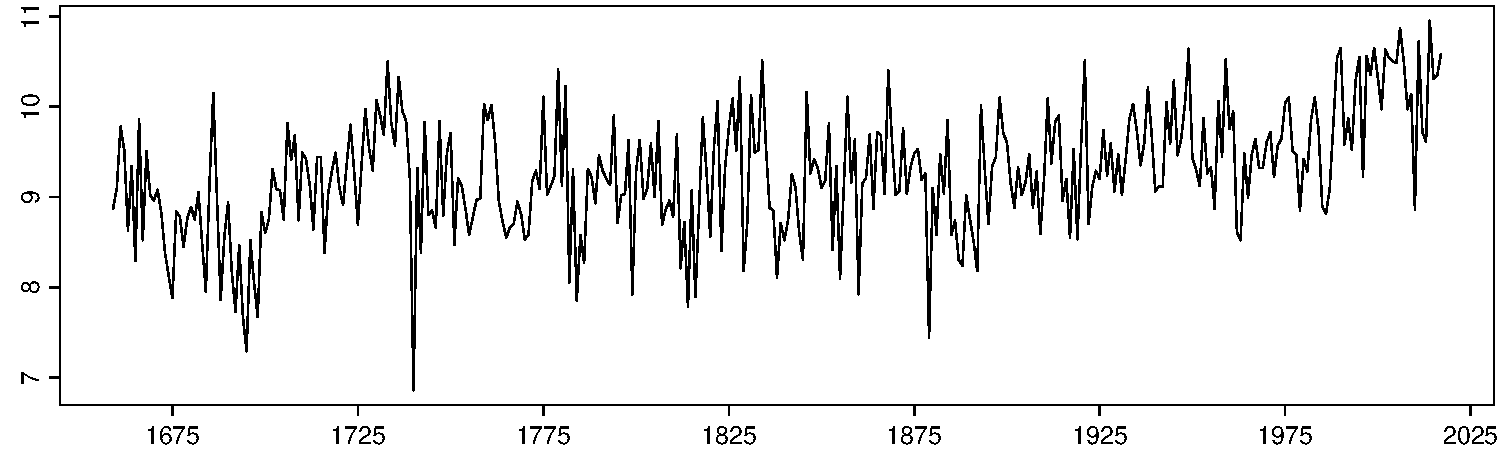
\includegraphics[width=0.9\textwidth]{Plots/temp_data.pdf}
\vspace{0.15cm}

\caption{Yearly mean temperature in Central England from 1659 to 2017 measured in $^\circ$C.}\label{temp_data}
\end{figure}


In this paper, we develop new methods to test for certain shape properties of a nonparametric time trend. We in particular construct a multiscale test which allows to identify local increases/decreases of the trend function. 
%We in particular construct a multiscale test for local increases/de\-creases of the trend function. The proposed test allows to identify, with a pre-specified statistical confidence, time regions where there is an increase/decrease in the trend. 
%identify subintervals on which the function $m$ deviates significantly from the null hypothesis of constancy. 
We develop our test in the context of the following model setting: We observe a time series $\{ Y_{t,T}: 1 \le t \le T \}$ of the form 
\begin{equation}\label{model-intro}
Y_{t,T} = m \Big( \frac{t}{T} \Big) + \varepsilon_t
\end{equation}
for $1 \le t \le T$, where $m: [0,1] \rightarrow \mathbb{R}$ is an unknown nonparametric regression function and the error terms $\varepsilon_t$ form a stationary time series process with $\ex[\varepsilon_t] = 0$. In a time series context, the design points $t/T$ represent the time points of observation and $m$ is a nonparametric time trend. As usual in nonparametric regression, we let the function $m$ depend on rescaled time $t/T$ rather than on real time $t$. A detailed description of model \eqref{model-intro} is provided in Section \ref{sec-model}.


Our multiscale test is developed step by step in Section \ref{sec-method}. Roughly speaking, the procedure can be outlined as follows: Let $H_0(u,h)$ be the hypothesis that $m$ is constant in the time window $[u-h,u+h] \subseteq [0,1]$, where $u$ is the midpoint and $2h$ the size of the window. In a first step, we set up a test statistic $\widehat{s}_T(u,h)$ for the hypothesis $H_0(u,h)$. In a second step, we aggregate the statistics $\widehat{s}_T(u,h)$ for a large number of different time windows $[u-h,u+h]$. We thereby construct a multiscale statistic which allows to test the hypothesis $H_0(u,h)$ simultaneously for many time windows $[u-h,u+h]$. In the technical part of the paper, we derive the theoretical properties of the resulting multiscale test. To do so, we come up with a proof strategy which combines strong approximation results for dependent processes with anti-concentration bounds for Gaussian random vectors. This strategy is of interest in itself and may be applied to other multiscale test problems for dependent data. As shown by our theoretical analysis, our multiscale test is a rigorous level-$\alpha$-test of the overall null hypothesis $H_0$ that $H_0(u,h)$ is simultaneously fulfilled for all time windows $[u-h,u+h]$ under consideration. Moreover, for a given significance level $\alpha \in (0,1)$, the test allows to make simultaneous confidence statements of the following form: We can claim, with statistical confidence $1-\alpha$, that there is an increase/decrease in the trend $m$ on all time windows $[u-h,u+h]$ for which the hypothesis $H_0(u,h)$ is rejected. Hence, the test allows to identify, with a pre-specified statistical confidence, time regions where the trend $m$ is increasing/decreasing. 


For independent data, multiscale tests have been developed in a variety of different contexts in recent years. In the regression context, \cite{ChaudhuriMarron1999,ChaudhuriMarron2000} introduced the so-called SiZer method which has been extended in various directions; see e.g.\ \cite{HannigMarron2006} where a refined distribution theory for SiZer is derived. \cite{HallHeckman2000} constructed a multiscale test on monotonicity of a regression function. \cite{DuembgenSpokoiny2001} developed a multiscale approach which works with additively corrected supremum statistics and derived theoretical results in the context of a continuous Gaussian white noise model. Rank-based multiscale tests for nonparametric regression were proposed in \cite{Duembgen2002} and \cite{Rohde2008}. More recently, \cite{ProkschWernerMunk2018} have constructed multiscale tests for inverse regression models. In the context of density estimation, multiscale tests have been investigated in \cite{DuembgenWalther2008}, \cite{RufibachWalther2010}, \cite{SchmidtHieber2013} and \cite{EckleBissantzDette2017} among others. 


Whereas a large number of multiscale tests for independent data have been developed in recent years, multiscale tests for dependent data are much rarer. Most notably, there are some extensions of the SiZer approach to a time series context. \cite{Rondonotti2004} and \cite{Rondonotti2007} have introduced SiZer methods for dependent data which can be used to find local increases/decreases of a trend and which may thus be regarded as an alternative to our multiscale test. However, these SiZer methods are mainly designed for data exploration rather than for rigorous statistical inference. Our multiscale method, in contrast, is a rigorous level-$\alpha$-test of the hypo\-thesis $H_0$ which allows to make simultaneous confidence statements about the time regions where the trend $m$ is increasing/decreasing. Some theoretical results for dependent SiZer methods have been derived in \cite{ParkHannigKang2009}, but only under a quite severe restriction: Only time windows $[u-h,u+h]$ with window sizes or scales $h$ are taken into account that remain bounded away from zero as the sample size $T$ grows. Scales $h$ that converge to zero as $T$ increases are excluded. This effectively means that only large time windows $[u-h,u+h]$ are taken into consideration. Our theory, in contrast, allows to simultaneously consider scales $h$ of fixed size and scales $h$ that converge to zero at various different rates. We are thus able to take into account time windows of many different sizes. \textcolor{red}{In Section \ref{subsec-method-comparison}, we compare our approach to SiZer methods in more detail.}


Our multiscale approach is also related to Wavelet-based methods: Similar to the latter, it takes into account different locations $u$ and resolution levels or scales $h$ simultaneously. However, while our multiscale approach is designed to test for local increases/decreases of a nonparametric trend, Wavelet methods are commonly used for other purposes. Among other things, they are employed for estimating/reconstructing nonparametric regression curves [see e.g.\ \cite{Donoho1995} or \cite{vonSachsMacGibbon2000}] and for change point detection [see e.g.\ \citet{ChoFryzlewicz2012}]. 


%Whereas a large number of multiscale tests for independent data have been developed in recent years, multiscale tests for dependent data are much rarer. Most notably, there are some extensions of the SiZer approach to a time series context. \cite{Rondonotti2004}, \cite{Rondonotti2007} and \cite{ParkHannigKang2009} have developed SiZer methods for dependent data which can be regarded as an alternative to our multiscale test. However, these SiZer methods are mainly designed for data exploration rather than rigorous statistical inference. Our multiscale method, in contrast, is a rigorous level-$\alpha$-test of the hypo\-thesis $H_0$, which is backed up by a complete asymptotic theory. Moreover, it allows to make simultaneous confidence statements about the time regions where the trend function $m$ is increasing/decreasing, which is not possible with the SiZer tools of \cite{Rondonotti2004}, \cite{Rondonotti2007} and \cite{ParkHannigKang2009}. Our multiscale approach is also related to Wavelet-based methods: It investigates the data on different intervals $[u-h,u+h]$. Similar to Wavelet-based procedures, it thus takes into account different locations $u$ and resolution levels $h$ simultaneously. Nevertheless, we are not aware of any Wavelet-based test for local increases/decreases of the nonparametric trend function in model \eqref{model-intro}. Wavelet methods have been used for other purposes in the literature such as estimating/reconstructing nonparametric regression functions [see e.g.\ \cite{Donoho1995} or \cite{vonSachsMacGibbon2000}] and change point detection [see e.g.\ \citet{ChoFryzlewicz2012}]. 


The test statistic of our multiscale method depends on the long-run error variance $\sigma^2 = \sum\nolimits_{\ell=-\infty}^{\infty} \cov(\varepsilon_0,\varepsilon_{\ell})$, which is usually unknown in practice. To carry out our multiscale test, we thus require an estimator of $\sigma^2$. Indeed, such an estimator is required for virtually all inferential procedures in the context of model \eqref{model-intro}. Hence, the problem of estimating $\sigma^2$ in model \eqref{model-intro} is of broader interest and has received a lot of attention in the literature; see \cite{MuellerStadtmueller1988}, \cite{Herrmann1992} and \cite{Hall2003} among many others. In Section \ref{sec-error-var}, 
%we discuss several estimators of $\sigma^2$ which are valid under different conditions on the error process $\{\varepsilon_t\}$. 
\textcolor{red}{we introduce a new difference-based estimator of $\sigma^2$ for the case that $\{ \varepsilon_t \}$ belongs to the class of AR($\infty$) processes}. This estimator improves on existing methods in several respects. 


The methodological and theoretical analysis of the paper is complemented by a simulation study in Section \ref{sec-sim} and an empirical application in Section \ref{sec-data}. In the simulation study, we examine the finite sample properties of our multiscale test and compare it to the dependent SiZer methods introduced in \cite{Rondonotti2004} and \cite{Rondonotti2007}. Moreover, we investigate the small sample performance of our estimator of $\sigma^2$ in the AR($p$) case and compare it to the estimator of \cite{Hall2003}. In Section \ref{sec-data}, we use our methods to analyse the temperature data from Figure \ref{temp_data} \textcolor{red}{as well as a sample of global temperature data}. 




%\setlength{\parindent}{10ex} 

\section{Introduction}\label{sec:intro}

Comparison of several regression curves is a classical topic in econometrics and statistics. In many cases of practical interest, the functional forms of the objective regression curves are unknown, hence, the parametric approach is not applicable. In this paper, we propose a novel approach that addresses this particular problem in a nonparametric context. Specifically, we present a new testing procedure for detecting differences between the nonparametric trends curves. 

In what follows, we consider a general panel framework with heterogeneous trends. Suppose we observe a panel of $n$ time series $\mathcal{T}_i = \{ (Y_{it},\X_{it}): 1 \le t \le T \}$ for\linebreak $1 \le i \le n$, where $Y_{it}$ are real-valued random variables and $\X_{it} = (X_{it,1},\ldots, X_{it, d})^\top$ are $d$-dimensional random vectors. Each time series $\mathcal{T}_i$ is modelled by the equation
\begin{equation}\label{eq:model}
Y_{it} = m_i \Big( \frac{t}{T} \Big) + \bfbeta_i^\top \X_{it} + \alpha_i + \varepsilon_{it}
\end{equation}
for $1 \le t \le T$, where $\bfbeta_i$ is a $d \times 1$ vector of unknown parameters, $\X_{it}$ is a $d\times 1$ vector of individual covariates or controls, $m_i$ is an unknown nonparametric (deterministic) trend function defined on $[0,1]$, $\alpha_i$ are so-called fixed effect error terms and \linebreak $\mathcal{E}_i = \{ \varepsilon_{it}: 1 \le t \le T \}$ is a zero-mean stationary error process. 


An important question in many applications is whether the observed time series have a common trend. In other words, the researchers would like to know if $m_i$ are the same for all $i$. \textcolor{red}{When there is evidence that this is not the case, one of the major related statistical problems is to determine which of the trends are different and whether we can group the time series with the similar trends together. Moreover,} when two trends $m_i$ and $m_j$ are not the same, it may also be relevant to know in which time regions they differ from each other. In this paper, we introduce new statistical methods to approach these questions. In particular, we develop a test of the hypothesis that all time trends in model \eqref{eq:model} are the same. In this setting, the null hypothesis is formulated as 
\begin{align}\label{eq:null}
H_0: m_1 = m_2 = \ldots = m_n,
\end{align}
whereas the alternative hypothesis is 
$$H_1: \text{ there exists } x\in [0, 1] \text{ such that } m_i (x) \neq m_j(x) \text{ for some } 1\leq i < j \leq n.$$

The method that we propose does not only allow to test whether the null hypothesis is violated. It also allows to detect, with a given statistical confidence, which time trends are different and in which time regions they differ. More specifically, for any given interval $[u-h, u+h] \subseteq [0,1]$, consider the hypothesis
\[ H_0^{[i, j]}(u, h): m_i(w) = m_j(w) \text{ for all } w \in [u-h, u+h]. \] 
Here, we can regard $h$ as a bandwidth, a common tuning parameter in nonparametric estimation. The given interval $\interval = [u-h, u+h] \subseteq [0,1]$ is then fully characterised by $u$, its center (a location parameter), and $h$, the bandwidth. In order to determine the regions where the time trends are different, we consider a broad range of pairs $(u, h)$ with the property that they fully cover the unit interval $[0, 1]$. Formally, let \linebreak $\grid := \{(u, h): \interval = [u-h, u+h] \subseteq [0,1]\}$ be a grid of location-bandwidth points such that 
\begin{align*}
\bigcup_{(u, h) \in \grid}  \interval = [0,1].
\end{align*}
We then reformulate our null hypothesis \eqref{eq:null} as
\begin{align*}
H_0: \ & \text{The hypotheses } H_0^{[i, j]}(u, h) \text{ hold true for all intervals }  \interval, (u, h) \in \grid, \\ & \text{ and for all } 1 \le i < j \le n. 
\end{align*} 
$H_0^{[i, j]}(u, h)$ can thus be viewed as a local null hypothesis that characterises the behaviour of two trend functions locally, whereas $H_0$ specified in \eqref{eq:null} is the global null hypothesis that is concerned with the comparison of all of the trends on the whole unit interval.

Trend comparison is a common statistical problem that arises in various contexts. For example, in economics the researchers compare trends in real gross domestic product across several countries \citep[][]{Grier1989}, in yield over time of US Treasury bills at different maturities \citep[][]{Park2009}, or the evolution of long-term interest rates in a number of countries \citep[][]{Christiansen1997}. In finance, comparison and subsequent classification of the trends of market fragmentation can be used to assess the market quality in the European stock market (\citeauthor{VogtLinton2017}, \citeyear{VogtLinton2017}, \citeyear{VogtLinton2020}). In climatology, the temperature time series in different geographical areas are investigated in the context of the regional and global warming trends \citep[][]{KarolyWu2005}. Finally, in industry, mobile phone providers are interested in finding the differences between the cell phone download activity in various locations \citep[][]{DegrasWu2012}.


In the statistical literature, the problem of testing whether the observed time series all have the same trend  has been widely studied, and tests for equality of trends or regression curves have been developed in \cite{HaerdleMarron1990}, \cite{Hall1990}, \linebreak \cite{Delgado1993} and \cite{DegrasWu2012} among many others. Versions of model \eqref{eq:model} with a parametric trend are considered in \cite{Vogelsang2005}, \cite{Sun2011} and \cite{Xu2012} among others. In the nonparametric context, \cite{LiChenGao2010}, \cite{Atak2011}, \cite{Robinson2012} and \cite{ChenGaoLi2012} studied panel models under the assumption that the observed time series have a common time trend. However, in many applications the restriction of including a common time trend in the model is questionable at best. For instance, when we observe a large number of time series it is reasonable to expect that at least some of the trends are different from the others. Consequently, it often makes sense to relax the assumption of a common trend, which leads to more flexible panel settings with heterogeneous trends. Such models have been studied, for example, in \cite{DegrasWu2012},  \cite{Zhang2012} and \cite{Hidalgo2014}. \cite{DegrasWu2012} consider the problem of testing $H_0$ in a model that is a special case of \eqref{eq:model} and does not include additional regressors. \cite{ChenWu2018} develop theory for a very similar model framework but under more general conditions on the error terms. \linebreak \cite{Zhang2012} investigate the problem of testing the hypothesis $H_0$ in a slightly restricted version of model \eqref{eq:model}, where $\bfbeta_i = \bfbeta$ for all $i$. All of these tests have an important drawback: they involve classical nonparametric estimation of the trend functions that depends on one or several bandwidth parameters which imposes a certain limit on the applicability of such tests since in most cases it is far from clear how to choose these parameters in an appropriate way. Contrary to the aforementioned methods, our multiscale testing procedure allows us to consider a large collection of bandwidths simultaneously avoiding the problem of choosing only one bandwidth altogether.

\textcolor{red}{In this paper, we introduce a multiscale method that allows us to test the hypotheses $H_0^{[i, j]}(u, h)$ in the model \eqref{eq:model} simultaneously for all pairs $(i, j)$ and all intervals $\interval$ under consideration in a statistically rigorous way. By using appropriate critical values that depend on the scale of the problem (i.e. the number of hypotheses tested simultaneously and the relationship between them), our methods accounts for the multiple testing problem which arises from considering multiple statistical tests and allows us to make simultaneous confidence statements. Moreover, we show that the suggested procedure for obtaining critical values leads to good theoretical properties of the proposed test: it has the correct (asymptotic) level and an (asymptotic) power of one against a certain class of local alternatives. Based on our test method, we further construct an algorithm which clusters the observed time series into groups with the same trend.}



Recently, \cite{KhismatullinaVogt2021} proposed a new inference method that allows researchers to detect differences between epidemic time trends in the context of the COVID-19 pandemic. In their paper, the authors present a statistically rigorous procedure that, similarly to ours, not only allows to compare trends across different countries, but to pinpoint the time intervals where the differences occur as well. Moreover, they also circumvent the need to pick a bandwidth parameter by using a multiscale testing approach. However, the model in \cite{KhismatullinaVogt2021} is only a special case of the model \eqref{eq:model} which includes neither the covariates $\X_{it}$, nor the fixed effects $\alpha_i$. Furthermore, the authors place major restriction on the error terms: in their model, $\varepsilon_{it}$ are independent across $t$. In contrast, our model \eqref{eq:model} can be regarded as a generalised version of the one in \cite{KhismatullinaVogt2021} that allows for a wider range of economic and financial applications.

%This is a general problem concerning essentially all tests based on nonparametric curve estimators. There are of course many theoretical results on optimal bandwidth choice for estimation purposes. However, the optimal bandwidth for curve estimation is usually not optimal for testing. Optimal bandwidth choice for tests is indeed an open problem, and only little theory for simple cases is available \citep[][]{GaoGijbels2008}. Since tests based on nonparametric curve estimators are commonly quite sensitive to the choice of bandwidth and theory for optimal bandwidth selection is not available, it appears preferable to work with bandwidth-free tests. A classical way to obtain a bandwidth-free test of the hypothesis $H_0$ is to use CUSUM-type statistics which are based on partial sum processes. This approach is taken in \cite{Hidalgo2014}. A more modern approach to obtain a bandwidth-free test is to employ multiscale methods.

%More specifically, the basic idea is as follows: Let $S_h$ be a test statistic for the null hypothesis of interest, which depends on the bandwidth $h$. Rather than considering only a single statistic $S_h$ for a specific bandwidth $h$, a multiscale approach simultaneously considers a whole family of statistics $\{S_h: h \in \mathcal{H} \}$, where $\mathcal{H}$ is a set of bandwidth values. The multiscale test then proceeds as follows: For each bandwidth or scale $h$, one checks whether $S_h > q_h(\alpha)$, where $q_h(\alpha)$ is a bandwidth-dependent critical value (for given significance level $\alpha$). The multiscale test rejects if $S_h > q_h(\alpha)$ for at least one scale $h$. The main theoretical difficulty in this approach is of course to derive appropriate critical values $q_h(\alpha)$. Specifically, the critical values $q_h(\alpha)$ need to be determined such that the multiscale test has the correct (asymptotic) level, that is, such that $\pr (S_h > q_h(\alpha) \text{ for some } h \in \mathcal{H} ) = (1-\alpha) + o(1)$. 


%Multiscale methods have been developed for a variety of different test problems in recent years. \cite{ChaudhuriMarron1999, ChaudhuriMarron2000} introduced the so-called SiZer method which has been extended in various directions; see for example \cite{HannigMarron2006} and \cite{Rondonotti2007}. \cite{HorowitzSpokoiny2001} proposed a multiscale test for the parametric form of a regression function. \cite{DuembgenSpokoiny2001} constructed a multiscale approach which works with additively corrected supremum statistics. This general approach has been very influential in recent years and has been further developed in numerous ways; see for example \cite{Duembgen2002}, \cite{Rohde2008} and \cite{ProkschWernerMunk2018} for multiscale methods in the regression context and \cite{DuembgenWalther2008}, \cite{RufibachWalther2010}, \cite{SchmidtHieber2013} and \cite{EckleBissantzDette2017} for methods in the context of density estimation. Importantly, all of these studies are restricted to the case of independent data. It turns out that it is highly non-trivial to extend the multiscale approach of \cite{DuembgenSpokoiny2001} to the case of dependent data. A first step into this direction has recently been made in \cite{KhismatullinaVogt2020}. They developed multiscale methods to test for local increases/decreases of the nonparametric trend function $m$ in the univariate time series model $Y_t = m(t/T) + \varepsilon_t$.  


To sum up, the main theoretical contribution of the current paper is the multiscale testing method that allows to make simultaneous confidence statements about which of the time trends are distinct and the regions where they differ. We believe that currently there are no equivalent statistical methods. Even though tests for equality of the trends have been developed already for a while, most existing procedures allow only to test whether the trend curves are all the same or not, but they almost never allow to infer which curves are different and where. To the best of our knowledge, the only two exceptions are \cite{KhismatullinaVogt2021}, whose contribution is briefly discussed above, and \cite{Park2009} who developed SiZer methods for the comparison of nonparametric trend curves in a significantly simplified version of the model \eqref{eq:model}. In addition to restricted model, \cite{Park2009} derive theoretical results for their analysis only for the special case of observing only two time series, whereas in other cases, the algorithm is provided without detailed proof.

The structure of the paper is as follows. Section \ref{sec:model} introduces the model setting and the necessary technical assumptions that are required for the theory. The multiscale test is developed step by step in Section \ref{sec:test}. The main theoretical results are presented in Section \ref{sec:theo}. To keep the discussion as clear as possible, we include in the main text of the paper only the essential parts of the theoretical arguments, and the technical details and extended proofs are deferred to the Appendix. \textcolor{red}{Section \ref{sec:clustering} describes a simple clustering algorithm that can be applied to group the time series with the similar trends together. We complement the theoretical analysis of the paper by a simulation study in Section \ref{sec:sim}, where we investigate the finite
sample properties of the test methods and the clustering algorithm from Sections \ref{sec:test} and \ref{sec:clustering}. Section \ref{sec:app} presents two empirical applications to illustrate the usage of our method: testing for common trend in the GDP growth data and cross-country trend comparison of the housing prices.} Section \ref{sec:conclusion} concludes.



\section{The model framework}\label{sec:model}


\subsection{Notation}


%Throughout the paper, we adopt the following notation. For a vector $\mathbf{v} = (v_1, \ldots, v_m)\in\reals^m$, we write $|\mathbf{v}|_q = \big(\sum_{i=1}^m v_i^q\big)^{1/q}$ to denote its $\ell_q$-norm and use the shorthand $|\mathbf{v}| = |\mathbf{v}|_2$ in the special case $q = 2$. For a random vector $\mathbf{V}$, we define its $\mathcal{L}^q$-norm by $\|\mathbf{V}\|_q = (\ex |\mathbf{V}|^q)^{1/q}$ and write $\|\mathbf{V}\| := \|\mathbf{V}\|_2$ in the case $q = 2$.


Throughout the paper, we adopt the following notation. For a vector $\mathbf{v} = (v_1, \ldots, v_m)\in\reals^m$, we write $\|\mathbf{v}\|_q = \big(\sum_{i=1}^m v_i^q\big)^{1/q}$ to denote its $\ell_q$-norm and use the shorthand $\|\mathbf{v}\| = \|\mathbf{v}\|_2$ in the special case $q = 2$. For a random variable $V$, we define its $\mathcal{L}^q$-norm by $\|V\|_q = (\ex |V|^q)^{1/q}$ and write $\|V\| := \|V\|_2$ in the case $q = 2$.


Let $\eta_t$ ($t \in \integers$) be independent and identically distributed ($\text{i.i.d.}$) random variables, write $\mathcal{F}_t  = (\ldots, \eta_{t-1}, \eta_t)$ and let $g: \reals^\infty \to \reals$ be a measurable function such that $g(\mathcal{F}_t) = g(\ldots, \eta_{t-1}, \eta_t)$ is a properly defined random variable. Following \cite{Wu2005}, we define the \textit{physical dependence measure} of the process $\{g(\mathcal{F}_t)\}_{t=-\infty}^\infty$ by
\begin{align}\label{eq:physical_dep}
\delta_q(g, t) = \| g(\mathcal{F}_t) - g(\mathcal{F}_t^\prime) \|_q,
\end{align}
where $\mathcal{F}_t^\prime  = (\ldots, \eta_{-1}, \eta^\prime_0, \eta_1, \ldots, \eta_t)$ is a coupled version of $\mathcal{F}_t$ with $\eta_0^\prime$ being an i.i.d.\ copy of $\eta_0$. Evidently, $\delta_q(g, t)$ measures the dependency of the random variable $g(\mathcal{F}_t)$ on the innovation term $\eta_0$. %, i.e., how replacing $\epsilon_0$ by an i.i.d. copy while keeping all other innovations in place affects the output $\mathbf{L}(\mathcal{F}_t)$.


\subsection{Model}\label{subsec:model_setting}


We observe a panel of $n$ time series $\mathcal{T}_i = \{(Y_{it}, \X_{it}): 1 \le t \le T \}$ of length $T$ for $1 \le i \le n$. Each time series $\mathcal{T}_i$ satisfies the model equation 
\begin{equation}\label{eq:model_full}
Y_{it} = \bfbeta^\top_i \X_{it} + m_i \Big( \frac{t}{T} \Big) + \alpha_i + \varepsilon_{it} 
\end{equation}
for $1 \le t \le T$, where $\bfbeta_i$ is a $d \times 1$ vector of unknown parameters, $\X_{it}$ is a $d\times 1$ vector of individual covariates, $m_i$ is an unknown nonparametric trend function defined on the unit interval $[0,1]$ with $\int_0^1 m_i(u) du = 0$ for all $i$, $\alpha_i$ is a (deterministic or random) intercept term and $\mathcal{E}_i = \{ \varepsilon_{it}: 1 \le t \le T \}$ is a zero-mean stationary error process. As common in nonparametric regression, the trend functions $m_i$ in model \eqref{eq:model_full} depend on rescaled time $t/T$ rather than on real time $t$; 
%Using rescaled time is equivalent to restricting the domain of the functions to the unit interval which in turn allows us to apply the usual asymptotic arguments. 
see e.g.\ \cite{Robinson1989}, \cite{Dahlhaus1997} and \cite{VogtLinton2014} for a discussion of rescaled time in nonparametric estimation. The condition $\int_0^1 m_i(u) du = 0$ is required for identification in the presence of the intercept terms $\alpha_i$. Without imposing this condition, one can freely shift the functions $m_i$ by any (positive or negative) constant $c_i$ while simultaneously subtracting this constant from $\alpha_i$:
\[ Y_{it} = [m_i(t/T) + c_i] + \bfbeta_i^\top \X_{it} + [\alpha_i - c_i] + \varepsilon_{it}. \]
The term $\alpha_i$ can be regarded as a fixed effect error term which captures unobserved characteristics of the time series $\mathcal{T}_i$ that remain constant over time. We allow the error terms $\alpha_i$ to be dependent across $i$ in an arbitrary way. \textcolor{red}{We also allow for an arbitrary dependence structure of the individual covariates $\X_{it}$ across $i$. Hence, %by including the fixed-effect terms $\alpha_i$ in the model equation \eqref{eq:model_full},
we allow the $n$ time series $\mathcal{T}_i$ in our panel to be correlated with each other. Whereas the variables $\alpha_i$ and $\X_{it}$ may be correlated across time series, the error processes $\mathcal{E}_i$ are assumed to be independent across $i$.} Technical conditions regarding the model are discussed below. Throughout the paper we restrict attention to the case where the number of time series $n$ in model \eqref{eq:model_full} is fixed. Extending our theoretical results to the case where $n$ slowly grows with the sample size $T$ is a possible topic for further research.


\subsection{Assumptions}\label{subsec:model_assumptions}


The error processes $\mathcal{E}_i = \{ \varepsilon_{it}: 1 \le t \le T\}$ satisfy the following conditions. 
\begin{enumerate}[label=(C\arabic*),leftmargin=1.05cm]
\item \label{C-err1} 
The variables $\varepsilon_{it}$ allow for the representation $\varepsilon_{it} = g_i(\mathcal{F}_{it})$, where $\mathcal{F}_{it} = (\ldots,\eta_{it-2}, \linebreak \eta_{it-1},\eta_{it})$, the variables $\eta_{it}$ are i.i.d.\ across $t$, and $g_i: \reals^\infty \rightarrow \reals$ is a measurable function. 
It holds that $\ex[\varepsilon_{it}] = 0$ and $\| \varepsilon_{it} \|_q \le C < \infty$ for some $q > 4$ and a sufficiently large constant $C$. 
\item \label{C-err2} The processes $\mathcal{E}_i = \{ \varepsilon_{it}: 1 \le t \le T\}$ are independent across $i$.
\end{enumerate}
Assumption \ref{C-err1} implies that the error processes $\mathcal{E}_i$ are stationary and causal (in the sense that $\varepsilon_{it}$ does not depend on future innovations $\eta_{is}$ with $s>t$). The class of error processes that satisfy condition \ref{C-err1} is very large. It includes linear processes, nonlinear transformations thereof, as well as a large variety of nonlinear processes such as Markov chain models and nonlinear autoregressive models \citep[][]{Wu2016}. Following \cite{Wu2005}, we impose conditions on the dependence structure of the error processes $\mathcal{E}_i$ in terms of the physical dependence measure $\delta_q(g_i, t)$ defined in \eqref{eq:physical_dep}. In particular, we assume the following: 
\begin{enumerate}[label=(C\arabic*),leftmargin=1.05cm]
\setcounter{enumi}{2}
\item \label{C-err3} For each $i$, it holds that $\sum\nolimits_{s \ge t} \delta_q(g_i, s) = O ( t^{-\gamma} (\log t)^{-A})$ with $q$ from \ref{C-err1}, where $A > \frac{2}{3} (1/q + 1 + \gamma)$ and $\gamma = \{q^2 - 4 + (q-2) \sqrt{q^2 + 20q + 4}\} / 8q$. 
\end{enumerate}
For fixed $i$ and $t$, the expression $\sum\nolimits_{s \ge t} \delta_q(g_i, s)$ measures the cumulative effect of the innovation $\eta_0$ on the variables $\varepsilon_{it}, \varepsilon_{it+1},\ldots$ in terms of the $\mathcal{L}^q$-norm. Condition \ref{C-err3} puts some restrictions on the decay of $\sum\nolimits_{s \ge t} \delta_q(g_i, s)$ (as a function of $t$) and in particular implies that $\sum\nolimits_{s \ge 0} \delta_q(g_i, s)$ is finite. It is fulfilled by a wide range of stationary processes $\mathcal{E}_i$. For a detailed discussion of \ref{C-err1}--\ref{C-err3} and some examples of error processes that satisfy these conditions, see \cite{KhismatullinaVogt2020}.


The covariates $\X_{it} = (X_{it,1},\ldots, X_{it, d})^\top$ are assumed to have the following properties. 
\begin{enumerate}[label=(C\arabic*),leftmargin=1.05cm]
\setcounter{enumi}{3}
\item \label{C-reg1} The variables $X_{it, j}$ allow for the representation $X_{it, j} = h_{ij}(\mathcal{G}_{it, j})$, where $\mathcal{G}_{it, j} = (\ldots, \xi_{it-1,j}, \xi_{it, j})$, the random variables $\xi_{it, j}$ are i.i.d.\ across $t$ and $h_{ij}: \reals^\infty \rightarrow \reals$ is a measurable function such that $X_{it, j}$ is well-defined. We use the notation $\X_{it} = \boldsymbol{h}_{i}(\mathcal{G}_{it})$ with $\boldsymbol{h}_i = (h_{i1}, \ldots, h_{id})^\top$ and $\mathcal{G}_{it} = (\mathcal{G}_{it,1}, \ldots, \mathcal{G}_{it, d})^\top$. It holds that $\ex [X_{it, j}]=0$ and $\| X_{it, j} \|_{q^\prime} <\infty$ for all $i$ and $j$, where $q^\prime > \max \{ 2, \theta q \}$ with $q$ from \ref{C-err1} and $\theta$ specified in \ref{C-grid} below.
%$q^\prime > \max\{ 2\theta, 4\}$ and all $j$, where $\theta$ is specified in Assumption \ref{C-grid} below.
\item \label{C-reg2} The matrix $\ex[\X_{it} \X_{it}^\top]$ is invertible for each $i$.
\item \label{C-reg3} For each $i$ and $j$, it holds that $\sum_{s=t}^{\infty} \delta_{q^\prime}(h_{ij}, s)= O(t^{-\alpha})$ for some $\alpha > 1/2 - 1/{q^\prime}$ with $q^\prime$ from \ref{C-reg1}.
\end{enumerate}
Assumption \ref{C-reg1} guarantees that the process $\{ \X_{it}: 1 \le t \le T \}$ is stationary and causal for each $i$. Similar to the restrictions on the error processes, we employ the definition of the physical dependence measure $\delta_{q^\prime}(h_{ij}, s)$ in Assumption \ref{C-reg3}, thus ensuring that the cumulative effect of the innovation $\xi_{i0}$ on the variables $\X_{i0}, \X_{i1}, \X_{i2},\ldots$ is finite. 


We finally impose some assumptions on the relationship between the covariates and the errors and on the trend functions $m_i$.
\begin{enumerate}[label=(C\arabic*),leftmargin=1.05cm]
\setcounter{enumi}{6}
\item \label{C-reg-err} The random variables $\Delta \X_{it} = \X_{it} - \X_{it-1}$ and $\Delta \varepsilon_{it} = \varepsilon_{it} - \varepsilon_{it-1}$ are uncorrelated, that is, $\cov(\Delta \X_{it}, \Delta \varepsilon_{it}) = \ex[\Delta \X_{it} \Delta \varepsilon_{it}] = 0$. 
\item \label{C-trend} The trend functions $m_i$ are continuously differentiable on $[0, 1]$ \textcolor{red}{and satisfy the property $\int_0^1m_i (u)du = 0$ for each $i$}.
%The innovation processes $\{ \eta_{it}: t \in \integers \}$ and $\{\xi_{it}: t \in \integers \}$ are independent for each $i$. This implies that the processes $\{\varepsilon_{it}: t \in \integers\}$ and $\{ \X_{it}: t \in \integers \}$ are independent for each $i$ as well. \textcolor{red}{Weaken this!}
%\item \label{C-reg-err2} Let $\zeta_{i, t} = (u_{it}, \eta_{it})^\top$. Define $\mathcal{I}_{it} = (\ldots, \zeta_{i, t-1}, \zeta_{i, t})$ and $\mathbf{U}_i(\mathcal{I}_{it}) =  \boldsymbol{h}_i(\mathcal{U}_{it})G_i(\mathcal{J}_{it})$. With this notation at hand, we assume that $\sum_{s=0}^\infty \delta_2(\mathbf{U}_i, s)<\infty$.
%\textcolor{red}{This assumption is not needed. See the proof of ??}
\end{enumerate}
%\textcolor{red}{Assumption \ref{C-reg-err1} is a slightly relaxed independence assumption: even though we do not require the covariates $\X_{it}$ to be completely independent with the error terms $\varepsilon_{it}$, our theoretical results depend upon them being uncorrelated. We in particular need this restriction in order to prove asymptotic consistency for the differencing estimator $\widehat{\bfbeta}_i$ of $\bfbeta_i$ proposed in Section \ref{subsec:para:beta}. In principle, it would be possible to relax this assumption even further, but that would involve much more complicated estimation procedure of $\bfbeta_i$ and more arduous technical arguments. Assumption \ref{C-reg-err2} ensures short-range dependence among the variables in our model. Again, we can interpret this as the fact that the cumulative effect of a single error on all future values is bounded.}
%We employ these assumptions to prove the main theoretical results in our paper. For detailed proofs, we refer the reader to the Appendix.


\begin{remark}
The conditions \ref{C-reg1}--\ref{C-reg3} can be relaxed to cover nonstationary regressors as well as stationary ones. For example, \ref{C-reg1} may then be replaced by
{\color{red}
\begin{enumerate}[label=(C\arabic*$^\ast$),leftmargin=1.15cm]
\setcounter{enumi}{3}
\item \label{C-reg1-star} The variables $X_{it, j}$ allow for the representation $X_{it, j} = h_{ij}(t; \mathcal{G}_{it, j})$, where $\mathcal{G}_{it, j} = (\ldots, \xi_{it-1,j}, \xi_{it, j})$, the random variables $\xi_{it, j}$ are i.i.d.\ across $t$ and $h_{ij}: \reals^\infty \rightarrow \reals$ is a measurable function such that $X_{it, j}$ is well-defined. We use the notation $\X_{it} = \boldsymbol{h}_{i}(t; \mathcal{G}_{it})$ with $\boldsymbol{h}_i = (h_{i1}, \ldots, h_{id})^\top$ and $\mathcal{G}_{it} = (\mathcal{G}_{it,1}, \ldots, \mathcal{G}_{it, d})^\top$. It holds that $\ex [X_{it, j}]=0$ and $\| X_{it, j} \|_{q^\prime} <\infty$ for all $i$, $j$ and $t$, where $q^\prime > \max \{ 2, \theta q \}$ with $q$ from \ref{C-err1} and $\theta$ specified in \ref{C-grid} below.
\end{enumerate}}
The other assumptions can be adjusted accordingly. Our main theoretical results will in principle still hold in this case, however, the complexity of the technical arguments will increase drastically. Hence, for the sake of clarity, we restrict our attention only to stationary  covariates $\X_{it}$. 
\end{remark}


\section{Testing procedure}\label{sec:test}

In this section, we develop a multiscale testing procedure for the problem of comparison of the trend curves $m_i$ in model \eqref{eq:model_full}.  As we will see, the proposed multiscale method does not only allow to test whether the \textcolor{red}{global} null hypothesis is violated. It also provides information on where violations occur. More specifically, it allows to identify, with a pre-specified confidence, (i) trend functions which are different from each other and (ii) time intervals where these trend functions differ.

\subsection{Preliminary steps}\label{subsec:test:prep}

Testing the null hypothesis $H_0: m_1 = m_2 = \ldots = m_n$ in model \eqref{eq:model_full} is a challenging task not only because it involves nonparametric estimation of the functions $m_i(\cdot)$, but also due to the presence of an unknown fixed term $\alpha_i$ and a vector of unknown parameters $\bfbeta_i$. It is clear that if $\alpha_i$ and $\bfbeta_i$ are known, the problem of testing for the common time trend would be greatly simplified. That is, we would test $H_0: m_1 = m_2 = \ldots = m_n$ in the model
\begin{align*}
Y_{it} - \alpha_i - \bfbeta_i^\top \X_{it} & =: Y_{it}^\circ\\
					& = m_i \Big( \frac{t}{T} \Big) + \varepsilon_{it}, 
\end{align*}
which is a standard nonparametric regression equation. However, in reality the variables $Y_{it}^\circ$ are not observed since the intercept $\alpha_i$ and the coefficients $\bfbeta_i$ are not known. Nevertheless, given appropriate estimators $\widehat{\alpha}_i$ and $\widehat{\bfbeta}_i$, we can consider
\begin{align*}
\widehat{Y}_{it} := Y_{it} -\widehat{\alpha}_i - \widehat{\bfbeta}_i^\top \X_{it} =(\bfbeta_i - \widehat{\bfbeta}_i)^\top \X_{it} + m_i \Big( \frac{t}{T} \Big) + \big( \alpha_i - \widehat{\alpha}_i \big) + \varepsilon_{it}. 
\end{align*}
Thus, the unobserved variables $Y_{it}^\circ$ can be approximated by $\widehat{Y}_{it}$, and in what follows we show that under some mild conditions on $\widehat{\alpha}_i$ and $\widehat{\bfbeta}_i$, this approximation is indeed sufficient for our analysis. 

But before we proceed further, we show how to construct consistent estimates $\widehat{\alpha}_i$ and $\widehat{\bfbeta}_i$. To begin with, we focus on the estimation of the vector of unknown parameters $\bfbeta_i$. We construct the estimator  $\widehat{\bfbeta}_i$ in the following way.

\textcolor{red}{For each $i$, we consider the time series $\Delta \mathcal{T}_i = \{(\Delta Y_{it}, \Delta \X_{it}): 2 \leq t \leq T\}$ of the first differences $\Delta Y_{it} = Y_{it} - Y_{i t-1}$ and $\Delta  \X_{it} =  \X_{it} -  \X_{it-1}$.} We can write
\begin{align*}
	\Delta Y_{it} = Y_{it} - Y_{i t-1} =\bfbeta_i^\top \Delta \X_{it} + \bigg(m_i \Big( \frac{t}{T} \Big) - m_i \Big(\frac{t-1}{T}\Big)\bigg) + \Delta \varepsilon_{it},
\end{align*}
where $ \Delta \varepsilon_{it} = \varepsilon_{it} - \varepsilon_{i t-1}$. Since $m_i$ is Lipschitz \textcolor{red}{by Assumption \ref{C-trend}}, we can use the fact that $ \big|m_i \big( \frac{t}{T} \big) - m_i \big(\frac{t-1}{T}\big) \big| = O\big(\frac{1}{T}\big)$ and rewrite 
\begin{align}\label{model_with_regs}
	\Delta Y_{it} = \bfbeta_i^\top \Delta \X_{it} + \Delta \varepsilon_{it} + O\Big(\frac{1}{T}\Big).
\end{align}

Now, for each $i$ we employ the least squares estimation method to estimate $\bfbeta_i$ in \eqref{model_with_regs}, treating $\Delta \X_{it}$ as the regressors and $\Delta Y_{it}$ as the response variable. That is, we propose the following differencing estimator:
\begin{align}\label{eq:beta:est}
\widehat{\bfbeta}_i = \Big( \sum_{t=2}^T \Delta \X_{it} \Delta \X_{it}^\top \Big)^{-1} \sum_{t=2}^T \Delta \X_{it} \Delta Y_{it}
\end{align}
In Lemma \ref{lemma-beta-rate} in the Appendix, we show that $\widehat{\bfbeta}_i$ is a consistent estimator of $\bfbeta_i$ with the property $\bfbeta_i - \widehat{\bfbeta}_i = O_p(T^{-1/2})$ under our assumptions. 

Next, given $\widehat{\bfbeta}_i$, consider an appropriate estimator $\widehat{\alpha}_{i}$ for the intercept $\alpha_i$ calculated by
\begin{align}
\widehat{\alpha}_i &= \frac{1}{T}\sum_{t=1}^T \big(Y_{it} - \widehat{\bfbeta}_i^\top \X_{it}\big) = \frac{1}{T}\sum_{t=1}^T \big(\bfbeta_i^\top \X_{it} - \widehat{\bfbeta}_i^\top \X_{it} + \alpha_i + m_i(t/T) + \varepsilon_{it}\big) \nonumber \\
&= \big(\bfbeta_i - \widehat{\bfbeta}_i \big)^\top\frac{1}{T}\sum_{t=1}^T  \X_{it} + \alpha_i + \frac{1}{T}\sum_{i=1}^T m_i(t/T) + \frac{1}{T}\sum_{i=1}^T \varepsilon_{it}. \label{eq:alpha:est}
\end{align}
Note that $\frac{1}{T}\sum_{i=1}^T \varepsilon_{it} = O_p(T^{-1/2})$ and $\frac{1}{T}\sum_{i=1}^T m_i(t/T) = O(T^{-1})$ due to Lipschitz continuity of $m_i$ and normalisation $\int_{0}^1 m_i(u)du = 0$. Furthermore, $\frac{1}{T}\sum_{t=1}^T  \X_{it} = O_p(1)$ by Chebyshev's inequality and $\widehat{\bfbeta}_i - \bfbeta_i = O_p (T^{-1/2})$. Plugging all these results together in \eqref{eq:alpha:est}, we get that $\widehat{\alpha}_i - \alpha_i = O_p(T^{-1/2})$. Thus, the unobserved variables \linebreak $Y_{it}^\circ := Y_{it} - \bfbeta_i^\top \X_{it} - \alpha_i = m_i(t/T) + \varepsilon_{it}$ can be well approximated by $\widehat{Y}_{it} $ since \linebreak $\widehat{Y}_{it} = Y_{it} -\widehat{\alpha}_i - \widehat{\bfbeta}_i^\top \X_{it} = Y_{it}^\circ + O_p(T^{-1/2})$.

We now turn to the estimator of the long-run error variance $\sigma_i^2 = \sum\nolimits_{\ell=-\infty}^{\infty} \cov(\varepsilon_{i0}, \varepsilon_{i\ell})$ which is necessary for the construction of the test statistics later on. For the moment, we assume that the long-run variance does not depend on $i$, that is $\sigma_i^2 = \sigma^2$ for all $i$. We will need this further for conducting the testing procedure properly. Nevertheless, we keep the indices throughout the paper in order to be congruous in notation. We further let $\widehat{\sigma}_i^2$ be an estimator of $\sigma_i^2$ which is computed from the constructed sample $\{ \widehat{Y}_{it}: 1 \le t \le T \}$. We thus regard $\widehat{\sigma}_i^2 = \widehat{\sigma}_i^2(\widehat{Y}_{i1},\ldots,\widehat{Y}_{iT})$ as a function of the variables $\widehat{Y}_{it}$ for $1 \le t \le T$. Hence, whereas the true long-run variance is the same for all time series, the estimators are different. Throughout the paper, we assume that $\widehat{\sigma}_i^2 = \sigma_i^2 + o_p(\rho_T)$, where the conditions on $\rho_T$ will be provided further in Section \ref{sec:theo}. Our theory works with any estimator $\widehat{\sigma}_i^2$ that has this property. 

We now discuss some possible choices of $\widehat{\sigma}_i^2$. Following \cite{Kim2016}, we can estimate $\sigma_i$ for each $i$ by a variant of the subseries variance estimator proposed first by \cite{Carlstein1986} and then extended by \cite{WuZhao2007}. Formally, we set
\begin{align}
\widehat{\sigma}_i^2 = \frac{1}{2(M-1)s_T}\sum_{m=1}^M \bigg[ \sum_{t = 1}^{s_T} & \Big(Y_{i(t + ms_T)} - Y_{i(t + (m-1)s_T)} \nonumber \\[-0.2cm] & - \widehat{\bfbeta}_i^\top\big(\X_{i(t+ms_T)} - \X_{i(t+(m-1)s_T)}\big) \Big)\bigg]^2, \label{eq:lrv}
\end{align}
where $s_T$ is the length of subseries and $M = \lfloor T/s_T\rfloor$ is the largest integer not exceeding $T/s_T$. As per the optimality result in \cite{Carlstein1986}, we set $s_T \asymp T^{1/3}$. For a finite sample, we choose $s_T = \lfloor T^{1/3}\rfloor$. According to  Lemma \ref{lemmaA:lrv} in Appendix, $\widehat{\sigma}_i^2$ is an asymptotically consistent estimator of $\sigma_i^2$ with the rate of convergence $O_p(T^{-1/3})$.

\textcolor{red}{The largest advantage of the subseries variance estimator described above is that it can be used without imposing any additional assumptions on the error processes $\mathcal{E}_i$. However, as noted in \cite{KhismatullinaVogt2020}, estimating the long-run error variance in the presence of a pronounced trend and under general weak dependence conditions is a particularly difficult problem. Estimators often tend to be quite imprecise. Hence, in practice we opt for imposing certain some time series models on the error processes $\mathcal{E}_i$. For example, we can assume that for each $i$ the error process $\mathcal{E}_i$ has the AR($\infty$) structure which covers a wide range of applications. In this case, it is possible to obtain more precise estimates $\widehat{\sigma}_i^2$ using the difference-based method described in \cite{KhismatullinaVogt2020}. %In our application examples, we choose to impose this restriction on the error terms.
The detailed discussion of the behaviour of such an estimator in the presence of a trend and comparison with other long-run variance estimators can be found in \cite{KhismatullinaVogt2020}.}

%According to  Lemma \ref{lemmaA:lrv} in Appendix, $\widehat{\sigma}_i^2$ is an asymptotically consistent estimator of $\sigma_i^2$ with the rate of convergence $O_p(T^{-1/3})$. Recall that the rate of convergence of $\widehat{\sigma}^2_i$ necessary for proving our theoretical results is $o_p(\rho_T)$ with $\rho_T = o(\sqrt{h_{\min}}/\log T)$. {\color{green}Hence, for our theory to work with this estimator, we need to put some restrictions on $\rho_T$. Specifically, we need to have \linebreak $T^{-1/3}/\rho_T = o(1)$ which can be translated to the following condition on the minimal bandwidth:
%\begin{align}\label{eq:hmin}
%h_{\min} \gg T^{-2/3}\log^{2+2\iota} T \text{ for some} \,\,\, \iota >0.
%\end{align} Remember that under Assumption \ref{C-h}, we have that $h_{\min} \gg T^{- \left(1 - \frac{2}{q}\right)}\log T$. Taking into account \eqref{eq:hmin}, we can rewrite Assumption \ref{C-h} as follows:

%\begin{enumerate}[label=(C\arabic*$^\ast$),leftmargin=1.40cm]
%\setcounter{enumi}{12}
%\item \label{C-h-star} $h_{\min} \gg \max\{ T^{-(1-\frac{2}{q})} \log T, T^{-2/3}\log^{2+2\iota}  T \}$, that is, $h_{\min} / \{ T^{-(1-\frac{2}{q})} \log T \} \rightarrow \infty$ with $q > 4$ defined in \ref{C-err2} and $h_{\min} / \{ T^{-2/3}\log^{2+2\iota}  T \} \rightarrow \infty$ for some $\iota >0$, and $h_{\max} < 1/2$.
%\end{enumerate}

%This means that we can for example have $\rho_T = T^{-1/3}\log^\iota T$, which is still a slower rate of convergence than $T^{-1/3}$. To sum up, under the Assumptions \ref{C-err1} - \ref{C-grid}, \ref{C-h-star}, the subseries variance estimator provided by \eqref{eq:lrv} satisfies the necessary conditions for Theorem \ref{theo:stat:global}, and thus can be used for the construction of our multiscale statistics $\widehat{\Psi}_{n, T}$.}


\subsection{Construction of the test statistics}\label{subsec:test:stat}

We are now ready to introduce the multiscale statistic for testing the hypothesis \linebreak $H_0: m_1 = m_2 = \ldots = m_n$. For any pair of time series $i$ and $j$ and for any location-bandwidth pair $(u, h)$, we define the kernel averages
\begin{align}\label{eq:psi_hat_ij}
 \widehat{\psi}_{ij, T}(u, h) = \sum\limits_{t=1}^T w_{t,T}(u, h)(\widehat{Y}_{it} - \widehat{Y}_{jt}),
 \end{align}
where $w_{t,T}(u, h)$ are local linear kernel weights calculated by the following formula:
\begin{equation}\label{eq:weights}
w_{t,T}(u, h) = \frac{\Lambda_{t,T}(u, h)}{ \{\sum\nolimits_{t=1}^T \Lambda_{t,T}(u, h)^2 \}^{1/2} }, 
\end{equation}
where
\[ \Lambda_{t,T}(u, h) = K\Big(\frac{\frac{t}{T}-u}{h}\Big) \Big[ S_{T,2}(u, h) - \Big(\frac{\frac{t}{T}-u}{h}\Big) S_{T,1}(u, h) \Big], \]
$S_{T,\ell}(u, h) = (Th)^{-1} \sum\nolimits_{t=1}^T K(\frac{\frac{t}{T}-u}{h}) (\frac{\frac{t}{T}-u}{h})^\ell$ for $\ell = 1,2$ and $K$ is a kernel function. As common in nonparametric estimation, we assume that $K$ has the following properties: 
\begin{enumerate}[label=(C\arabic*),leftmargin=1.05cm]
\setcounter{enumi}{8}
\item \label{C-ker} The kernel $K$ is non-negative, symmetric about zero and integrates to one. Moreover, it has compact support $[-1,1]$ and is Lipschitz continuous, that is,\linebreak $|K(v) - K(w)| \le C_K |v-w|$ for any $v, w \in \reals$ and some constant $C_K > 0$.
\end{enumerate} 
Assumption \ref{C-ker} allows us to use usual kernel functions such as rectangular, Epanechnikov and Gaussian kernels.

We regard the kernel average $\widehat{\psi}_{ij, T}(u, h)$ as a measure of the distance between the two trend curves $m_i$ and $m_j$ on the interval $\interval = [u-h, u+h]$. However, instead of working directly with the kernel averages $\widehat{\psi}_{ij, T}(u, h)$, we replace them by their normalised and corrected version:
\begin{align}\label{eq:psi_zero_ij}
\hat{\psi}^0_{ij, T}(u, h) =  \Big|\frac{\widehat{\psi}_{ij, T}(u, h)}{(\widehat{\sigma}_i^2 + \widehat{\sigma}_j^2)^{1/2}}\Big| - \lambda(h).
\end{align}
Here, $\lambda(h) = \sqrt{2 \log \{ 1/(2h) \}}$ is an additive correction term that balances the significance of many test statistics that correspond to different values of bandwidth parameters (see the discussion on this topic and comparison between multiscale testing procedures with and without this correction term in \citet{KhismatullinaVogt2020}).

We now aggregate the test statistics $\hat{\psi}^0_{ij, T}(u, h)$ for all $i$ and $j$ and a wide range of different locations $u$ and bandwidths (scales) $h$:
\begin{align}\label{eq:Psi_hat}
	\widehat{\Psi}_{n,T} = \max_{1 \le i < j \le n}\max_{(u, h) \in \mathcal{G}_T} \hat{\psi}^0_{ij, T}(u, h),
\end{align}

In \eqref{eq:Psi_hat}, $\grid$ stands for the set of location-bandwidth pairs $(u, h)$ that was mentioned in Section \ref{sec:intro}. We use the subscript $T$ in $\grid$ to point out that the choice of the grid depends on the sample size $T$. Specifically, throughout the paper, we suppose that $\grid$ is some subset of $\grid^{\text{full}} = \{ (u, h): u = t/T \text{ and } h = s/T \text{ for some } 1 \le t, s \le T \text{ such that } \linebreak h \in [h_{\min},h_{\max}] \}$, where $h_{\min}$ and $h_{\max}$ denote some minimal and maximal bandwidth value, respectively. As was already discussed in Section \ref{sec:intro}, we assume that the set of intervals $\{\interval = [u-h, u+h]: (u, h) \in \grid\}$ covers the whole unit interval. Furthermore, for our theoretical results, we require the following additional conditions to hold:
\begin{enumerate}[label=(C\arabic*),leftmargin=1.05cm]
\setcounter{enumi}{9}

\item \label{C-grid} $|\mathcal{G}_T| = O(T^\theta)$ for some arbitrarily large but fixed constant $\theta > 0$, where $|\mathcal{G}_T|$ denotes the cardinality of $\mathcal{G}_T$. 

\item \label{C-h} $h_{\min} \gg T^{-(1-\frac{2}{q})} \log T$, that is, $h_{\min} / \{ T^{-(1-\frac{2}{q})} \log T \} \rightarrow \infty$ with $q > 4$ defined in \ref{C-err2} and $h_{\max} = o(1)$.

\end{enumerate}
Assumption \ref{C-grid} places relatively mild restrictions on the grid $\grid$: we allow the grid to grow with the sample size but only at a polynomial rate $T^\theta$ with fixed $\theta$. This is not a severe constraint because under this limitation, we can still work with the full set of location-bandwidth points $\grid = \grid^{\text{full}}$ which is more than enough for most applied problems. Assumption \ref{C-h} is concerned with the minimal and the maximal bandwidths that we use for our analysis. Specifically, according to Assumption \ref{C-h}, we can choose the minimal bandwidth $h_{\min}$ that converges to zero slower than $T^{-(1-\frac{2}{q})} \log T$ as the sample size $T$ goes to infinity. \textcolor{red}{The maximal bandwidth $h_{\max}$ needs only to slowly converge to zero as the sample size grows, hence, in finite samples it can be picked quite large.}

Note that the value $\max_{(u, h) \in \mathcal{G}_T} \hat{\psi}^0_{ij, T}(u, h)$ simultaneously takes into account all intervals $\interval = [u- h, u+h]$ with $(u, h) \in \mathcal{G}_T$. Thus, it can be interpreted as a global distance measure between the two curves $m_i$ and $m_j$, and the test statistics $\widehat{\Psi}_{n,T}$ is then defined as the maximal distance between any pair of curves $m_i$ and $m_j$ with $i \ne j$.

In Section \ref{subsec:test:test}, we show how to test the null hypothesis $H_0: m_1 =m_2 = \ldots = m_n$ using the multiscale test statistics $\widehat{\Psi}_{n,T}$.

\subsection{The testing procedure}\label{subsec:test:test}


Let $Z_{it}$ for $1 \le t \le T$ and $1 \le i \le n$ be independent standard normal random variables which are independent of the error terms $\varepsilon_{js}$ and the covariates $\X_{js}$ for all $1 \leq s \leq T $ and $1 \leq j \leq n$. Denote the empirical average of the variables $Z_{i1},\ldots, Z_{iT}$ by $\bar{Z}_{i,T} = T^{-1} \sum_{t=1}^T Z_{it}$. To simplify the notation, we will omit the subscript $T$ in $\bar{Z}_{i,T}$ in what follows. Similarly as with $\hat{\psi}^0_{ij, T}(u, h)$, for each $i$ and $j$, we introduce the normalised and corrected Gaussian kernel averages 
\begin{align}\label{eq:phi_zero_ij}
\phi^0_{ij, T}(u, h) =  \bigg|\frac{\phi_{ij, T}(u, h)}{(\sigma_i^2 + \sigma_j^2)^{1/2}}\bigg| - \lambda(h),
\end{align}
where 
\begin{align}\label{eq:phi_ij}
\phi_{ij, T}(u, h) = \sum\nolimits_{t=1}^T w_{t,T}(u, h) \, \big\{ \sigma_i (Z_{it} - \bar{Z}_i) - \sigma_j (Z_{jt} - \bar{Z}_j) \big\}
\end{align}
with $w_{t, T}(u, h)$ defined in \eqref{eq:weights}. 

Next, in the same way as in \eqref{eq:Psi_hat}, we define the global Gaussian test statistic
\begin{align}\label{eq:Phi}
\Phi_{n,T} = \max_{1 \le i < j \le n}\max_{(u, h) \in \mathcal{G}_T} \phi^0_{ij, T}(u, h)
\end{align}
and denote its $(1-\alpha)$-quantile by $q_{n,T}(\alpha)$.

Our multiscale test of the hypothesis $H_0: m_1 = m_2 = \ldots = m_n$ is defined as follows: 
\begin{center}
\begin{minipage}[c][0.75cm][c]{13cm}
\textit{For a given significance level $\alpha \in (0,1)$, we reject $H_0$ if $\widehat{\Psi}_{n,T} > q_{n,T}(\alpha)$.}
\end{minipage}
\end{center}

\begin{remark}\label{rem:simpl}
To prove the theoretical results in Section \ref{sec:theo}, we will use the following fact. By our assumption that the long-run variance $\sigma_i^2$ does not depend on $i$ \linebreak (i.e. $\sigma_i^2 = \sigma^2_j = \sigma^2$), we can rewrite the Gaussian normalised kernel averages \eqref{eq:phi_zero_ij} as
\[\phi^0_{ij, T}(u, h) = \frac{1}{\sqrt{2}} \Big|\sum\nolimits_{t=1}^T w_{t,T}(u, h) \, \big\{ (Z_{it} - \bar{Z}_i) - (Z_{jt} - \bar{Z}_j) \big\}\Big| - \lambda(h), \] 
which means that the distribution of the Gaussian test statistics does not depend neither on the data $\mathcal{T}_i =\{ (Y_{it}, \X_{it}) : 1\leq t \leq T)\}, \mathcal{T}_j =\{ (Y_{jt}, \X_{jt}) : 1\leq t \leq T)\}$, nor on any unknown quantities such as $\sigma^2_i$ or $\sigma_j^2$, and thus can be regarded as known. In addition to exploiting this fact while proving the theoretical results, we will also use it for \textcolor{red}{(approximately) calculating the quantiles of $\Phi_{n, T}$ by the Monte Carlo simulations in Sections \ref{sec:sim} and \ref{sec:app}. However, throughout the paper, we will stick to the definition \eqref{eq:phi_zero_ij} for the sake of similarity to $\hat{\psi}^0_{ij, T}(u, h)$.}%, which involves the long-run variances $\sigma_i$ and $\sigma_j$.
\end{remark}

\begin{remark}
By construction, the $(1-\alpha)$ Gaussian quantile $q_{n, T}(\alpha)$ depends not only on the number of times series considered $n$ and the sample size $T$, but on the choice of the set of location-bandwidth pairs $\grid$ as well. However, we do not explicitly include this dependence since we believe it will only lead to the unnecessary complication of the notation. 
\end{remark}

\subsection{Locating the differences}\label{subsec:test:loc}

Suppose we reject the null hypothesis $H_0$. This fact does not provide us with a lot of information about the behaviour of the trend functions $m_i$: \textcolor{red}{we can only state with a given statistical confidence that some of the trend functions are not equal somewhere on $[0, 1]$,} but we can not tell which of the functions are different and where they differ. Hence, we need an additional step in the testing procedure in order to locate those differences.

Formally, for a given pair of time series $(i, j)$ and for any given interval \linebreak $\interval = [u-h, u+h]$ such that $(u, h) \in \grid$ we consider the hypothesis 
\[ H_0^{[i, j]}(u, h): m_i(w) = m_j(w) \text{ for all } w \in [u-h, u+h]. \] 
We view $H_0^{[i, j]}(u, h)$ as the local null hypothesis because \textcolor{red}{it compares two trend functions $m_i$ and $m_j$ locally, on the interval $\interval = [u-h, u+h]$.} In contrast, we refer to $H_0$ introduced in \eqref{eq:null} as the global null hypothesis.

We define the multiscale test of the hypothesis $H_0^{[i, j]}(u, h)$ as follows: 
\begin{center}
\begin{minipage}[c][1.25cm][c]{13cm}
\textit{For a given significance level $\alpha \in (0,1)$, we reject $H_0^{[i, j]}(u, h)$ if \linebreak $\hat{\psi}^0_{ij, T}(u, h) > q_{n,T}(\alpha)$.}
\end{minipage}
\end{center}

For each pair of time series $(i, j)$, denote the set of intervals $\interval$ that consists of the intervals where we reject $H_0^{[i, j]}(u, h)$ at a significance level $\alpha$ by $\mathcal{S}^{[i, j]}(\alpha)$. We will prove later in Section \ref{sec:theo}, that we can make the following confidence statements:

\begin{center}
\begin{minipage}[c][1.45cm][c]{13cm}
\textit{We can state with (asymptotic) probability at least $1-\alpha$ that for all $i, j, \linebreak1\leq i < j \leq n$, we have that $m_i$ and $m_j$ differ on all of the intervals $\interval \in \mathcal{S}^{[i, j]}(\alpha)$.}
\end{minipage}
\end{center}


\subsection{Implementation of the test in practice}\label{subsec:test:impl}

In practice, we implement the test procedure described in Sections \ref{subsec:test:test} and \ref{subsec:test:loc} in the following way. 
\begin{enumerate}[label=\textit{Step \arabic*.}, leftmargin=1.45cm]
\item Fix a significance level $\alpha \in (0, 1)$. 
\item Compute the (approximated) quantile $q_{n, T}(\alpha)$ by Monte Carlo simulations. Specifically, draw a large number $N$ (say $N=5000$) of samples of independent standard normal random variables $\{Z_{it}^{(\ell)} : 1 \le t \le T, \, 1 \le i \le n \}$ for $1 \le \ell \le N$. For each sample $\ell$, compute the value $\Phi_{n,T}^{(\ell)}$ of the Gaussian test statistics $\Phi_{n, T}$ and store them. Calculate the empirical $(1-\alpha)$-quantile $\hat{q}_{n, T}(\alpha)$ from the stored values $\{ \Phi_{n, T}^{(\ell)}: 1 \le \ell \le N \}$. Use $\hat{q}_{n, T}(\alpha)$ as an approximated value of the quantile $q_{n, T}(\alpha)$.
\item Carry out the test for the global hypothesis $H_0$ by calculating $\widehat{\Psi}_{n, T}$ and checking if $\widehat{\Psi}_{n, T} > \hat{q}_{n, T}(\alpha)$. Reject the null if this is the case.
\item For each $i, j,\, 1 \le i < j \le n$, and each $(u, h) \in \grid$, carry out the test for the local null hypothesis $H_0^{[i, j]}(u, h)$ by checking if $\hat{\psi}^0_{ij, T}(u, h)> \hat{q}_{n, T}(\alpha)$. For each pair of time series $(i, j)$, find the set of intervals $\mathcal{S}^{[i, j]}(\alpha)$ that consists of the intervals $\mathcal{I}_{(u, h)}$ where we reject $H_0^{[i, j]}(u, h)$. 
%Store the test results in the variable $r_{ij, T}(u, h) = \mathds{1}( |\hat{\psi}_{ij, T}^0(u, h)| > q_{n, T}(\alpha))$, where $\mathds{1}(\cdot)$ is an indicator function that is equal to $1$ if the condition inside the brackets is met and $0$ otherwise.
\item Display the results. One of the possible ways to do that is to produce a separate plot for each of the pairwise comparisons and draw only the intervals where we reject the corresponding local null. Formally, on each of the plots that present the results of the comparison of time series $i$ and $j$, we display the intervals $\interval = [u- h, u+h] \in \mathcal{S}^{[i, j]}(\alpha)$, i.e.\ the (rescaled) time intervals where we reject $H_0^{[i, j]}(u, h)$.
\end{enumerate}

\textcolor{red}{In some cases, the number of intervals in the set $\mathcal{S}^{[i, j]}(\alpha)$ may be quite large, making the visual representation of the graphical summary of the results more complicated. To overcome this drawback, we work with the subset of minimal intervals $\mathcal{S}^{[i, j]}_{\text{min}}(\alpha) \subseteq \mathcal{S}^{[i, j]}(\alpha)$ which is constructed as follows: As in \cite{Duembgen2002}, we call an interval $\mathcal{I}_{(u, h)} \in \mathcal{S}^{[i, j]}(\alpha)$ minimal if there is no other interval $\mathcal{I}_{(u^\prime, h^\prime)} \in \mathcal{S}^{[i, j]}(\alpha)$ such that $\mathcal{I}_{(u^\prime, h^\prime)} \subset \mathcal{I}_{(u, h)}$. We denote the set of all minimal intervals by $\mathcal{S}^{[i, j]}_{\text{min}}(\alpha)$. All of our theoretical results can be rewritten using the subset of minimal intervals $\mathcal{S}^{[i, j]}_{\text{min}}(\alpha)$ instead of $\mathcal{S}^{[i, j]}(\alpha)$.}


\section{Theoretical properties of the test}\label{sec:theo}


In order to investigate the theoretical properties of our multiscale test, we introduce the auxiliary statistic
\begin{align}\label{eq:Phi_hat}
\widehat{\Phi}_{n,T} = \max_{1 \le i < j \le n}  \max_{(u, h) \in \mathcal{G}_T} \widehat{\phi}^0_{ij, T}(u, h),
\end{align}
where
\begin{equation*}%\label{eq:phi_hat_ij_zero}
\widehat{\phi}^0_{ij, T}(u, h) =\bigg| \frac{\widehat{\phi}_{ij, T}(u, h)} {\{ \widehat{\sigma}_i^2 + \widehat{\sigma}_j^2 \}^{1/2}} \bigg| - \lambda(h)
\end{equation*}
and
\begin{align*}
\widehat{\phi}_{ij, T}(u, h) 
 & = \sum_{t=1}^T w_{t,T}(u, h) \big\{ (\varepsilon_{it} - \bar{\varepsilon}_i) + (\bfbeta_i - \widehat{\bfbeta}_i)^\top (\X_{it} - \bar{\X}_{i}) \\[-0.4cm]
 & \phantom{= \sum_{t=1}^T w_{t,T}(u, h) \big\{} - (\varepsilon_{jt} - \bar{\varepsilon}_j) -  (\bfbeta_j - \widehat{\bfbeta}_j)^\top (\X_{jt} - \bar{\X}_{j}) \big\}.
\end{align*}
We here use the notation $\bar{\varepsilon}_i = \bar{\varepsilon}_{i,T} := T^{-1} \sum_{t=1}^T \varepsilon_{it}$ and $\bar{\X}_{i} =  \bar{\X}_{i, T} := T^{-1}\sum_{t=1}^T  \X_{it}$. By construction, it holds that $\widehat{\phi}_{ij, T}(u, h) = \widehat{\psi}_{ij, T}(u, h)$ under $H_0^{[i, j]}(u, h)$. This implies that $\widehat{\Phi}_{n,T}$ is identical to $\widehat{\Psi}_{n,T}$ under the global null $H_0$. Hence, in order to determine the distribution of our main test statistic $\widehat{\Psi}_{n,T}$ under $H_0$, we can study the auxiliary statistic $\widehat{\Phi}_{n,T}$. The following theorem shows that the distribution of $\widehat{\Phi}_{n,T}$ is close to the distribution of the Gaussian statistic $\Phi_{n,T}$ introduced in \eqref{eq:Phi}. 


%However, $\widehat{\Phi}_{n,T}$ depends on the covariates $\X_{it}$ whereas the Gaussian version $\Phi_{n,T}$ that is used to calculate critical values for our test (defined in \eqref{eq:Phi}) is independent of them. This is the reason why we need to introduce additional intermediate test statistic that does not include the covariates, therefore, connecting $\widehat{\Phi}_{n,T}$ and $\Phi_{n,T}$. This intermediate test statistics will play an important role in the proof of our main theoretical result.

%Formally, for each $i, j$ we construct the kernel averages as 
%\[\doublehat{\phi}_{ij, T}(u, h) = \sum_{t=1}^T w_{t,T}(u, h) \big\{ (\varepsilon_{it} - \bar{\varepsilon}_i) - (\varepsilon_{jt} - \bar{\varepsilon}_j)  \big\}. \]
%We can view these kernel averages as constructed under the null from the unobserved variables $\doublehattwo{Y}_{it}$ and  $\doublehattwo{Y}_{jt}$ given by the following formula: 
%\begin{align*}
%\doublehattwo{Y}_{it} :&= Y_{it} - \bfbeta_i^\top \X_{it} -  \frac{1}{T}\sum_{t=1}^T \big(Y_{it} - \bfbeta_i^\top \X_{it}\big) =\\
%&=m_i \Big( \frac{t}{T} \Big)  - \frac{1}{T}\sum_{t=1}^T  m_i \Big( \frac{t}{T} \Big) + \varepsilon_{it} - \frac{1}{T}\sum_{t=1}^T \varepsilon_{it}.
%\end{align*}

%The intermediate statistic $\doublehattwo{\Phi}_{n, T}$ is then defined as 
%\begin{align}\label{eq:Phi_doublehat}
%\doublehattwo{\Phi}_{n,T} &= \max_{1 \le i < j \le n}\max_{(u, h) \in \mathcal{G}_T} \Bigg\{\bigg|\frac{\doublehat{\phi}_{ij, T}(u, h)}{\big(\doublehattwo{\sigma}_i^2 + \doublehattwo{\sigma}_j^2\big)^{1/2}}\bigg| - \lambda(h)\Bigg\}
%\end{align}
%with $\doublehattwo{\sigma}_i^2$ being an estimator of the long-run error variance $\sigma_i^2 = \sum\nolimits_{\ell=-\infty}^{\infty} \cov(\varepsilon_{i0}, \varepsilon_{i\ell})$ which is computed from the unobserved sample $\{ \doublehattwo{Y}_{it} : 1 \le t \le T \}$. We thus regard $\doublehattwo{\sigma}_i^2 = \doublehattwo{\sigma}_i^2(\doublehattwo{Y}_{i1},\ldots,\doublehattwo{Y}_{iT})$ as a function of the variables $\doublehat{Y}_{it}$ for $1 \le t \le T$. As with the estimator $\widehat{\sigma}_i^2$, we assume that $\doublehattwo{\sigma}_i^2 = \sigma_i^2 + o_p(\rho_T)$ with $\rho_T = o(\sqrt{h_{\min}}/\log T)$. 

%The statistics $\doublehattwo{\Phi}_{n,T}$ can thus be viewed as a version of the statistic $\widehat{\Phi}_{n,T}$ without the covariates. We formally prove that these two statistics are close in Proposition \ref{propA:intermediate2}.

%Now we can formally state our main theoretical result which characterises the asymptotic behaviour of the statistic $\widehat{\Phi}_{n,T}$. 

\begin{theorem}\label{theo:stat:global}
Let \ref{C-err1}--\ref{C-h} be fulfilled and assume that $\sigma_i^2 = \sigma^2$, $\widehat{\sigma}_i^2 = \sigma^2_i + o_p(\rho_T)$ with $\rho_T = o(\sqrt{h_{\min}}/\log T)$ for all $i$. Then  
\begin{equation*}
\sup_{x \in \reals} \big| \pr(\widehat{\Phi}_{n, T} \le x) - \pr(\Phi_{n,T} \le x) \big| = o(1),
\end{equation*}
%\[ \pr \big( \widehat{\Phi}_{n,T} \le q_{n,T}(\alpha) \big) = (1 - \alpha) + o(1). \]
\end{theorem}
Theorem \ref{theo:stat:global} is the principal instrument for deriving theoretical properties of our multiscale test. Its proof is provided in the Appendix. 

%Here, we briefly present the main arguments.

%First, we show that the distribution of the intermediate statistics $\doublehattwo{\Phi}_{n, T}$ introduced in \eqref{eq:Phi_doublehat} is indeed close to the distribution of $\widehat{\Phi}_{n, T}$, and therefore, we can approximate the distribution of $\widehat{\Phi}_{n, T}$ with the help of $\doublehattwo{\Phi}_{n, T}$.

%Second, we show that we can replace $\doublehattwo{\Phi}_{n, T}$ by an identically distributed version $\widetilde{\Phi}_{n, T}$ which is close to the Gaussian statistics $\Phi_{n, T}$ defined in \eqref{eq:Phi}. Formally, by the means of strong approximation theory derived in \cite{BerkesLiuWu2014} we prove that there exist statistics $\widetilde{\Phi}_{n, T}$ which are distributed as $\doublehattwo{\Phi}_{n, T}$ for any $T \ge 1$ and which have the property that 
%\begin{align}\label{eq:proof1}
%\big| \widetilde{\Phi}_{n, T} - \Phi_{n,T} \big| = o_p( \delta_T),
%\end{align}
%where $\delta_T = o(1)$.

%Then, we employ the anti-concentration results derived in \cite{Chernozhukov2015} in order to show that $\Phi_{n,T}$ does not concentrate too strongly in small regions of the form $[x-delta_T, x\delta_T, x+\delta_T]$. Or, in other words, it holds that 
%\begin{align}\label{eq:proof2}
%\sup_{x \in \reals} \pr \big( | \Phi_{n,T} - x | \le \delta_T \big) = o(1)
%\end{align}
%Taking \eqref{eq:proof1} together with \eqref{eq:proof2} and the fact that $\widetilde{\Phi}_{n, T}$ has the same distribution as $\doublehattwo{\Phi}_{n, T}$ yields that 
%\begin{equation*}
%\sup_{x \in \reals} \big| \pr(\doublehattwo{\Phi}_{n, T} \le x) - \pr(\Phi_{n,T} \le x) \big| = o(1). 
%\end{equation*}
 
%And finally, by the fact mentioned in the beginning of this proof that the distribution of the intermediate statistics $\doublehattwo{\Phi}_{n, T}$ is close to the distribution of $\widehat{\Phi}_{n, T}$, we conclude that 
%\begin{equation*}
%\sup_{x \in \reals} \big| \pr(\widehat{\Phi}_{n, T} \le x) - \pr(\Phi_{n,T} \le x) \big| = o(1),
%\end{equation*}
%which immediately implies the statement of Theorem \ref{theo:stat:global}.

\begin{remark}
The proof of Theorem \ref{theo:stat:global} builds on two important theoretical results: strong approximation theory developed in \cite{BerkesLiuWu2014} and anti-concentration results proved in \cite{Chernozhukov2015}. These results were already combined together for the purpose of developing the multiscale test for dependent data in \cite{KhismatullinaVogt2020}. We can say that our proof can be regarded as a further development of the proof strategy in \cite{KhismatullinaVogt2020} where they proposed a similar testing procedure for investigating properties of the trend function in one time series. We extend their theoretical result not only by working with multiple time series, but also by including the covariate terms in the model \eqref{eq:model}. Hence, our proof strategy builds on the similar stones but is much more technically involved.
\end{remark}

Now we examine the theoretical properties of the testing procedure proposed in \linebreak Sections \ref{subsec:test:test} and \ref{subsec:test:loc} with the help of Theorem \ref{theo:stat:global}. The following proposition 
%(which is a direct consequence of Theorem \ref{theo:stat:global}) 
states that our test has correct (asymptotic) size.

\begin{prop}\label{prop:test}
Suppose that the conditions of Theorem \ref{theo:stat:global} are satisfied. Then under $H_0$, we have
\[ \pr \big( \widehat{\Psi}_{n,T} \le q_{n,T}(\alpha) \big) = (1 - \alpha) + o(1). \]
\end{prop}

The next proposition characterises the behaviour of our multiscale test under a certain class of local alternatives. To formulate it, we consider a sequence of pairs of functions $m_ i := m_{i,T}$ and $m_ j := m_{j,T}$ that depend on the sample size and that are locally sufficiently far from each other.

\begin{prop}\label{prop:test:power}
Let the conditions  of Theorem \ref{theo:stat:global} be satisfied. Moreover, assume that for some pair of indices $i$ and $j$, the functions $m_ i = m_{i,T}$ and $m_ j = m_{j,T}$ have the following property: There exists $(u, h) \in \mathcal{G}_T$ with $[u-h, u+h] \subseteq [0,1]$ such that $m_{i,T}(w) - m_{j,T}(w) \ge c_T \sqrt{\log T/(Th)}$ for all $w \in [u-h, u+h]$ or $m_{j,T}(w) - m_{i,T}(w) \ge c_T \sqrt{\log T/(Th)}$ for all $w \in [u-h, u+h]$, where $\{c_T\}$ is any sequence of positive numbers with $c_T \rightarrow \infty$. Then 
\[ \pr \big( \widehat{\Psi}_{n,T} \le q_{n,T}(\alpha) \big) = o(1). \]
\end{prop}

%Proof of Proposition \ref{prop:test:power} is provided in the Appendix.

Finally, we turn our attention to the local null hypotheses $H_0^{[i, j]}(u, h)$. Since we are testing many hypotheses at the same time, we would like to bound the probability of making even one false discovery. For this purpose, we employ the notion of the family-wise error rate (FWER) which is equal to the probability of making one or more type I errors. Formally, the FWER is defined as
\begin{align*} 
\text{FWER}(\alpha) = \pr \Big(\exists \,  i, j \in \{1, \ldots, n \}, (u, h) \in \grid : & \, \interval \in \mathcal{S}^{[i, j]}(\alpha) \\ & \, \text{and } H_0^{[i, j]}(u, h) \text { is true}\Big).
\end{align*}

We say that the FWER is controlled at level $\alpha$ if $\text{FWER}(\alpha) \leq \alpha$. The following result assures that for our testing procedure, this is indeed the case.

\begin{prop}\label{prop:test:fwer}
Suppose that the conditions  of Theorem \ref{theo:stat:global} are satisfied. Then 
\[ \textnormal{FWER}(\alpha) \leq \alpha. \]
\end{prop}

%Proposition \ref{prop:test:fwer} is a direct consequence of Theorem \ref{theo:stat:global}. Nevertheless, the detailed proof of this proposition is provided in the Appendix. 

The following corollary is an immediate consequence of Proposition \ref{prop:test:fwer} and gives the theoretical justification necessary for making simultaneous confidence statements about the locations of the differences between the trends.

\begin{corollary}\label{corollary1}
Under the conditions of Theorem \ref{theo:stat:global}, for any given $\alpha \in (0,1)$, we have
%\[ \pr\Big( \forall (i, jj, k, k) \in \indexset: \text{ If } |\hat{\psi}_{ijk, T}| > c_{T,\textnormal{Gauss}}(\alpha, h_k), \text{ then } (i, j, k) \notin \indexset_0 \Big) \ge 1 - \alpha + o(1) \]
\begin{align*}
\pr\Big( \forall \, i, j \in \{1, \ldots, n\}, (u, h) \in \grid \text{ s.t. } H_0^{[i, j]}(u, h) \text{ is true}: & \, \hat{\psi}^0_{ij, T}(u, h) \le q_{n,T}(\alpha) \Big) \\ & \qquad \quad \quad \ge 1 - \alpha + o(1).
\end{align*}
%Hence, with asymptotic probability at least $1-\alpha$, the two intensity functions $\lambda_i$ and $\lambda_j$ differ on the interval $\mathcal{I}_k$ for all $(i, j, k) \in \indexset$ for which the test rejects $H_0^{(ijk)}$. 
\end{corollary} 


With the help of Corollary \ref{corollary1}, we are able to make simultaneous confidence statements about which of the trends are different and where:

\begin{center}
\begin{minipage}[c][1.25cm][c]{13cm}
\textit{We can state with (asymptotic) probability at least $1-\alpha$ that for all $i, j$, $1 \le i < j \le n$, $m_i$ and $m_j$ differ on all of the intervals $\interval \in \mathcal{S}^{[i, j]}(\alpha)$.}
\end{minipage}
\end{center}



\section{Clustering}\label{sec:clustering}

Consider a situation in which the null hypothesis $H_0: m_1 = m_2 = \ldots = m_n$ is violated. Even though some of the trend functions are different in this case, part of them may still be the same. Put differently, there may be groups of time series which have the same time trend. Formally speaking, we define a group structure as follows: There exist sets or groups of time series $G_1,\ldots, G_N$ with $N \le n$ and $\{1,\ldots, n\} = \mathbin{\dot{\bigcup}}_{\ell=1}^{N} G_\ell$ such that for each $1 \le \ell \le N$,
\[ m_i = f_\ell \quad \text{for all } i \in G_\ell, \]
where $f_\ell$ are group-specific trend functions. Hence, the time series which belong to the group $G_\ell$ all have the same time trend $f_\ell$. Throughout the section, we suppose that the group-specific trend functions $f_\ell$ have the following properties: For each $\ell$, $f_\ell = f_{\ell,T}$ is a Lipschitz continuous function with $\int_0^1 f_{\ell,T}(w) dw = 0$. In particular, it holds that $|f_{\ell,T}(v) - f_{\ell,T}(w)| \le L |v-w|$ for all $v, w \in [0,1]$ and some constant $L < \infty$ that does not depend on $T$. Moreover, for any $\ell \ne \ell^\prime$, the trends $f_{\ell,T}$ and $f_{\ell^\prime,T}$ are assumed to differ in the following sense: There exists $(u, h) \in \mathcal{G}_T$ with $\mathcal{I}_{(u, h)} = [u-h, u+h] \subseteq [0,1]$ such that $f_{\ell,T}(w) - f_{\ell^\prime,T}(w) \ge c_T \sqrt{\log T/(Th)}$ for all $w \in \mathcal{I}_{(u, h)}$ or $f_{\ell^\prime,T}(w) - f_{\ell,T}(w) \ge c_T \sqrt{\log T/(Th)}$ for all $w \in \mathcal{I}_{(u, h)}$, where $0 < c_T \rightarrow \infty$.


In many applications, it is natural to suppose that there is a group structure in the data. In this case, a particular interest lies in estimating the unknown groups from the data at hand. In what follows, we combine our multiscale methods with a clustering algorithm to achieve this. {\color{red}More specifically, we use the aggregated multiscale statistics $\max_{(u, h) \in \mathcal{G}_T}\hat{\psi}^0_{ij, T}(u, h)$ calculated for each $i$ and $j$, $1\leq i < j \leq n$,} as distance measures which are fed into a hierarchical clustering algorithm. To describe the algorithm, we first need to introduce the notion of a dissimilarity measure: Let $S \subseteq \{1,\ldots, n\}$ and $S^\prime \subseteq \{1,\ldots, n\}$ be two sets of time series from our sample. We define a dissimilarity measure between $S$ and $S^\prime$ by setting 
{\color{red}\begin{equation}\label{dissimilarity}
\widehat{\Delta}(S,S^\prime) = \max_{\substack{i \in S, \\ j \in S^\prime}} \Big(\max_{(u, h) \in \mathcal{G}_T}\hat{\psi}^0_{ij, T}(u, h)\Big). 
\end{equation}}
This is commonly called a complete linkage measure of dissimilarity. Alternatively, we may work with an average or a single linkage measure. We now combine the dissimilarity measure $\widehat{\Delta}$ with a hierarchical agglomerative clustering (HAC) algorithm which proceeds as follows: 
\vspace{10pt}

\noindent \textit{Step $0$ (Initialisation):} Let $\widehat{G}_i^{[0]} = \{ i \}$ denote the $i$-th singleton cluster for $1 \le i \le n$ and define $\{\widehat{G}_1^{[0]},\ldots,\widehat{G}_n^{[0]} \}$ to be the initial partition of time series into clusters. 
\vspace{5pt}

\noindent \textit{Step $r$ (Iteration):} Let $\widehat{G}_1^{[r-1]},\ldots,\widehat{G}_{n-(r-1)}^{[r-1]}$ be the $n-(r-1)$ clusters from the previous step. Determine the pair of clusters $\widehat{G}_{\ell}^{[r-1]}$ and $\widehat{G}_{{\ell}^\prime}^{[r-1]}$ for which 

\[ \widehat{\Delta}(\widehat{G}_{\ell}^{[r-1]},\widehat{G}_{{\ell}^\prime}^{[r-1]}) = \min_{1 \le k < k^\prime \le n-(r-1)} \widehat{\Delta}(\widehat{G}_{k}^{[r-1]},\widehat{G}_{k^\prime}^{[r-1]}) \]  
and merge them into a new cluster. 
\vspace{10pt}

\noindent Iterating this procedure for $r = 1,\ldots, n-1$ yields a tree of nested partitions \linebreak $\{\widehat{G}_1^{[r]},\ldots$ $\ldots,\widehat{G}_{n-r}^{[r]}\}$, which can be graphically represented by a dendrogram. Roughly speaking, the HAC algorithm merges the $n$ singleton clusters $\widehat{G}_i^{[0]} = \{ i \}$ step by step until we end up with the cluster $\{1,\ldots, n\}$. In each step of the algorithm, the closest two clusters are merged, where the distance between clusters is measured in terms of the dissimilarity $\widehat{\Delta}$. We refer the reader to Section 14.3.12 in \cite{HastieTibshiraniFriedman2009} for an overview of hierarchical clustering methods. 


When the number of groups $N$ is known, we estimate the group structure $\{G_1,\ldots, G_N\}$ by the $N$-partition $\{\widehat{G}_1^{[n-N]},\ldots,\widehat{G}_{N}^{[n-N]}\}$ produced by the HAC algorithm. When $N$ is unknown, we estimate it by the $\widehat{N}$-partition $\{\widehat{G}_1^{[n-\widehat{N}]},\ldots,\widehat{G}_{\widehat{N}}^{[n-\widehat{N}]}\}$, where $\widehat{N}$ is an estimator of $N$. The latter is defined as 
\[ \widehat{N} = \min \Big\{ r = 1,2,\ldots \Big| \max_{1 \le \ell \le r} \widehat{\Delta} \big( \widehat{G}_\ell^{[n-r]} \big) \le q_{n,T}(\alpha) \Big\}, \]
where we write $\widehat{\Delta}(S) = \widehat{\Delta}(S,S)$ for short and $q_{n,T}(\alpha)$ is the $(1-\alpha)$-quantile of $\Phi_{n,T}$ defined in Section \ref{subsec:test:test}. 

The following proposition summarises the theoretical properties of the estimators $\widehat{N}$ and $\{ \widehat{G}_1,\ldots,\widehat{G}_{\widehat{N}} \}$, where we use the shorthand $\widehat{G}_\ell = \widehat{G}_\ell^{[n-\widehat{N}]}$ for $1 \le \ell \le \widehat{N}$. 
\begin{prop}\label{prop:clustering:1}
Let the conditions of Theorem \ref{theo:stat:global} be satisfied. Then 
\[ \pr \Big( \big\{ \widehat{G}_1,\ldots,\widehat{G}_{\widehat{N}} \big\} = \{ G_1,\ldots, G_N \} \Big) \ge (1-\alpha) + o(1) \]
and 
\[ \pr \big( \widehat{N} = N \big) \ge (1-\alpha) + o(1). \]
\end{prop}
This result allows us to make statistical confidence statements about the estimated clusters $\{ \widehat{G}_1,\ldots,\widehat{G}_{\widehat{N}} \}$ and their number $\widehat{N}$. In particular, we can claim with asymptotic confidence $\ge 1 - \alpha$ that the estimated group structure is identical to the true group structure. Note that it is possible to let the significance level $\alpha$ depend on the sample size $T$ in Proposition \ref{prop:clustering:1}. In particular, we can allow $\alpha = \alpha_T$ to converge slowly to zero as $T \rightarrow \infty$, in which case we obtain that $\pr ( \{ \widehat{G}_1,\ldots,\widehat{G}_{\widehat{N}} \} = \{ G_1,\ldots, G_N \} ) \rightarrow 1$ and $\pr ( \widehat{N} = N ) \rightarrow 1$. The proof of Proposition \ref{prop:clustering:1} can be found in the Appendix.

Our multiscale methods do not only allow us to compute estimators of the unknown groups $G_1,\ldots, G_N$. They also provide information on the locations where two group-specific trend functions $f_\ell$ and $f_{\ell^\prime}$ differ from each other. To turn this claim into a mathematically precise statement, we need to introduce some notation. First of all, note that the indexing of the estimators $\widehat{G}_1,\ldots,\widehat{G}_{\widehat{N}}$ is completely arbitrary. We could, for example, change the indexing according to the rule $\ell \mapsto \widehat{N} - \ell + 1$. In what follows, we suppose that the estimated groups are indexed such that $P( \widehat{G}_\ell = G_\ell \text{ for all } \ell ) \ge (1-\alpha) + o(1)$. Proposition \ref{prop:clustering:1} implies that this is possible without loss of generality. Keeping this convention in mind, we define the sets 
{\color{red}\[ \mathcal{A}_{n,T}^{[\ell,\ell^\prime]}(\alpha)= \Big\{ (u, h) \in \mathcal{G}_T: \widehat{\psi}^0_{ij, T}(u, h) > q_{n,T}(\alpha) \text{ for some } i \in \widehat{G}_\ell, j \in \widehat{G}_{\ell^\prime} \Big\} \]
and  
\[ \mathcal{S}^{[\ell,\ell^\prime]}_{n, T}(\alpha) = \big\{ \mathcal{I}_{(u, h)} = [u-h, u+h]: (u, h) \in \mathcal{A}_{n,T}^{[\ell,\ell^\prime]}(\alpha) \big\} \]
%\[ \Pi_{n,T}(\ell,\ell^\prime) = \big\{ \mathcal{I}_{(u, h)} = [u-h, u+h]: (u, h) \in \mathcal{A}_{n,T}(\ell,\ell^\prime) \big\} \]
for $1 \le \ell < \ell^\prime \le \widehat{N}$. An interval $\mathcal{I}_{(u, h)}$ is contained in $\mathcal{S}^{[\ell,\ell^\prime]}_{n, T}(\alpha)$ if our multiscale test indicates a significant difference between the trends $m_i$ and $m_j$ on the interval $\mathcal{I}_{(u, h)}$ for some $i \in \widehat{G}_\ell$ and $j \in \widehat{G}_{\ell^\prime}$. Put differently, $\mathcal{I}_{(u, h)} \in \mathcal{S}^{[\ell,\ell^\prime]}_{n, T}(\alpha)$ if the test suggests a significant difference between the trends of the $\ell$-th and the $\ell^\prime$-th group on the interval $\mathcal{I}_{(u, h)}$. We further let
\[ E_{n,T}^{[\ell,\ell^\prime]}(\alpha) = \Big\{ \forall \mathcal{I}_{(u, h)} \in \mathcal{S}^{[\ell,\ell^\prime]}_{n, T}(\alpha): f_\ell(v) \ne f_{\ell^\prime}(v) \text{ for some } v \in \mathcal{I}_{(u, h)} = [u-h, u+h] \Big\} \]
be the event that the group-specific time trends $f_\ell$ and $f_{\ell^\prime}$ differ on all intervals $\mathcal{I}_{(u, h)} \in \mathcal{S}^{[\ell,\ell^\prime]}_{n, T}(\alpha)$.} With this notation at hand, we can make the following formal statement whose proof is given in the Appendix. \textcolor{blue}{(add proof)} 
%\begin{prop}\label{prop:clustering:2}
%Under the conditions of Theorem \ref{theo:stat:global}, the event 
%\[ E_{n,T} = \Big\{ \bigcap_{1 \le \ell < \ell^\prime \le \widehat{N}} E_{n,T}(\ell,\ell^\prime) \Big\} \cap \Big\{ \widehat{N} = N \text{ and } \widehat{G}_\ell = G_\ell \text{ for all } \ell \Big\} \]
%asymptotically occurs with probability $\ge 1-\alpha$, that is, 
%\[ \pr \big( E_{n,T} \big) \ge (1 - \alpha) + o(1). \]
%\end{prop}
{\color{red}\begin{prop}\label{prop:clustering:2}
Under the conditions of Theorem \ref{theo:stat:global}, the event 
\[ E_{n,T}(\alpha) = \Big\{ \bigcap_{1 \le \ell < \ell^\prime \le \widehat{N}} E_{n,T}^{[\ell,\ell^\prime]}(\alpha) \Big\} \cap \Big\{ \widehat{N} = N \text{ and } \widehat{G}_\ell = G_\ell \text{ for all } \ell \Big\} \]
asymptotically occurs with probability $\ge 1-\alpha$, that is, 
\[ \pr \big( E_{n,T}(\alpha) \big) \ge (1 - \alpha) + o(1). \]
\end{prop}}
The statement of Proposition \ref{prop:clustering:2} remains to hold true when the sets of intervals %$\Pi_{n,T}(\ell,\ell^\prime)$
\textcolor{red}{$\mathcal{S}^{[\ell,\ell^\prime]}_{n, T}(\alpha)$} are replaced by the corresponding sets of minimal intervals. According to Proposition \ref{prop:clustering:2}, the sets %$\Pi_{n,T}(\ell,\ell^\prime)$
\textcolor{red}{$\mathcal{S}^{[\ell,\ell^\prime]}_{n, T}(\alpha)$} allow us to locate, with a pre-specified confidence, time regions where the group-specific trend functions $f_\ell$ and $f_{\ell^\prime}$ differ from each other. In particular, we can claim with asymptotic confidence $\ge 1 - \alpha$ that the trend functions $f_\ell$ and $f_{\ell^\prime}$ differ on all intervals \textcolor{red}{$\mathcal{I}_{(u, h)} \in \mathcal{S}^{[\ell,\ell^\prime]}_{n, T}(\alpha)$}. %$\mathcal{I}_{(u, h)} \in \Pi_{n,T}(\ell,\ell^\prime)$.

\section{\textcolor{red}{Simulations}}\label{sec:sim}

In this Section, we present the results for the simulation study for the testing method described in Section \ref{sec:test}. The simulation design is as follows. We generate data from the model $Y_{it} =m_i(\frac{t}{T})  + \beta_i X_{it} +  \alpha_i  + \varepsilon_{it}$, where the number of time series $i$ is set to $n = 15$ and we consider different time series lengths $T$. For simplification purposes, we assume that there is only one covariate variable $X_{it}$, and we set the unknown parameter $\beta_i = 1$ for all $i$. We also assume that the fixed--effect term $\alpha_i$ is equal to $0$ in all time series. For each $i$, the errors $\varepsilon_{it}$ are drawn from the AR(1) model $\varepsilon_{it} = a \varepsilon_{i, t-1} + \eta_{it}$, where $a = 0.25$ and the innovations $\eta_{it}$ are i.i.d.\ normally distributed with mean $0$ and variance $0.25$. Furthermore, for each $i$, the covariates $X_{it}$ also follow an AR($1$) process $X_{it} = a_x X_{i, t-1} + \zeta_{it}$, where $a_x = 0.5$ and the innovations $\zeta_{it}$ are i.i.d.\ normally distributed with mean $0$ and variance $1$. We assume that the covariates $X_{it}$ and the error terms $\varepsilon_{js}$ are independent from each other for all $1 \leq i,j \leq n$ and $1 \leq t, s \leq T$.

To generate data under the null $H_0: m_1 = \ldots = m_n$, we let $m_i = 0$ for all $i$ without loss of generality. To produce data under the alternative, we define $m_1(u) = b \, (u - 0.5) $ with $b = 0.75, 1, 1.25$ and set $m_i = 0$ for all $i \ne 1$. Hence, all trend functions are the same except for $m_1$ which is an increasing linear function. We use a linear function as the normalisation constraint $\int_0^1 m_1(u) du = 0$ is directly satisfied in this case. We simulate $S = 5000$ data samples and carry out the test for each simulated sample.

\begin{table}[t]
\footnotesize{
\begin{center}
\caption{Size of the multiscale test for $n=15$ time series, different sample sizes $T$ and nominal sizes $\alpha$.}
\label{tab:size}
\renewcommand{\arraystretch}{1.2}
% latex table generated in R 4.0.5 by xtable 1.8-4 package
% 
\begin{tabular}{cccc}
  \hline
  & \multicolumn{3}{c}{nominal size $\alpha$} \\
 $T$ & 0.01 & 0.05 & 0.1 \\
 \hline
250 & 0.023 & 0.094 & 0.156 \\ 
  500 & 0.019 & 0.067 & 0.120 \\ 
  1000 & 0.016 & 0.052 & 0.111 \\ 
   \hline
\end{tabular}

\end{center}}
\footnotesize{
\begin{center}
\caption{Power of the multiscale test for $n=15$ time series, different sample sizes $T$ and nominal sizes $\alpha$. Each panel corresponds to a different slope parameter $b$.}\label{tab:power}
\begin{subtable}[b]{0.32\textwidth}
\centering
\caption{$b = 0.75$}\label{tab:power_075}
\renewcommand{\arraystretch}{1.2}
% latex table generated in R 4.0.5 by xtable 1.8-4 package
% 
\begin{tabular}{cccc}
  \hline
  & \multicolumn{3}{c}{nominal size $\alpha$} \\
 $T$ & 0.01 & 0.05 & 0.1 \\
 \hline
100 & 0.035 & 0.112 & 0.181 \\ 
  250 & 0.203 & 0.418 & 0.549 \\ 
  500 & 0.715 & 0.886 & 0.939 \\ 
   \hline
\end{tabular}

\end{subtable}
\begin{subtable}[b]{0.32\textwidth}
\centering
\caption{$b = 1.00$}\label{tab:power_100}
\renewcommand{\arraystretch}{1.2}
% latex table generated in R 4.0.5 by xtable 1.8-4 package
% 
\begin{tabular}{cccc}
  \hline
  & \multicolumn{3}{c}{nominal size $\alpha$} \\
 $T$ & 0.01 & 0.05 & 0.1 \\
 \hline
100 & 0.105 & 0.270 & 0.376 \\ 
  250 & 0.635 & 0.840 & 0.901 \\ 
  500 & 0.994 & 0.999 & 0.999 \\ 
   \hline
\end{tabular}

\end{subtable}
\begin{subtable}[b]{0.32\textwidth}
\centering
\caption{$b = 1.25$}\label{tab:power_125}
\renewcommand{\arraystretch}{1.2}
% latex table generated in R 4.0.5 by xtable 1.8-4 package
% 
\begin{tabular}{cccc}
  \hline
  & \multicolumn{3}{c}{nominal size $\alpha$} \\
 $T$ & 0.01 & 0.05 & 0.1 \\
 \hline
100 & 0.052 & 0.137 & 0.220 \\ 
  250 & 0.209 & 0.434 & 0.560 \\ 
  500 & 0.690 & 0.867 & 0.918 \\ 
   \hline
\end{tabular}

\end{subtable}
\end{center}}
\vspace{-0.4cm}
\end{table}
%
The testing procedure is implemented as follows. In the first step, we estimate the unknown parameter $\beta_i$ for each $i$ using the first-differencing method described in Section~\ref{subsec:test:prep}. Given $\widehat{\beta}_i$, we obtain an estimator $\widehat{\alpha}_i$ of the fixed-effect term $\alpha_i$ calculated as in \eqref{eq:alpha:est}. We then work with the augmented time series $Y_{it}^o = Y_{it} - \widehat{\alpha}_i - \widehat{\beta}_i X_{it}$.

In the second step, we construct the multiscale test statistics using an Epanechnikov kernel and the grid defined as $\mathcal{G}_T = U_T \times H_T$ with 
\begin{align*}
U_T & = \big\{ u \in [0,1]: u = \textstyle{\frac{t}{T}} \text{ for some } t \in \naturals \big\} \\
H_T & = \big\{ h \in \big[ \textstyle{\frac{\log T}{T}}, \textstyle{\frac{1}{4}} \big]:  h = \textstyle{\frac{5 t -3}{T}} \text{ for some } t \in \naturals \big\}. 
\end{align*}
Hence, each interval $\mathcal{I}_{u, h} = [u-h, u+h]$ contains $5, 15, 25, \ldots$ data points. Furthermore, since the errors follow an AR($1$) process, we estimate the long-run variances $\sigma_i^2$ using the difference-based estimator proposed in \cite{KhismatullinaVogt2020} setting the tuning parameters $q$ and $r$ to $10$ and $25$, respectively.

We then turn to the computation of the critical values for our test. Specifically, we simulate $5000$ values of the statistic $\Phi_{n,T}$ defined in \eqref{eq:Phi} and compute their empirical $(1-\alpha)$ quantile $\widehat{q}_{n,T}(\alpha)$. Note that in general the statistic $\Phi_{n,T}$ depends on the long-run error variances $\sigma_i^2$. However, as stated in the Remark \ref{rem:simpl}, under the assumption that the long-run error variance is known to be the same across $i$ (that is, $\sigma_i^2 = \sigma^2$ for all $i$), this is not the case. Under this assumption, we can simplify the formula for the kernel averages $\phi^0_{ij, T}(u, h)$ so that it involves no unknown parameters. Hence, the distribution of $\Phi_{n, T}$ does not depend on any unknown quantities, including the value of the long-run variance $\sigma_i^2$.

%Under this assumption, we can estimate $\sigma^2$ by $\widehat{\sigma}^2 = (\sum_{i = 1}^n\widehat{\sigma_i}^2)/n$, and the Gaussian statistic $\Phi_{n,T}$ simplifies to $\Phi_{n,T} = \max_{1 \le i < j \le n} \Phi_{ij, T}$ with $\Phi_{ij, T} = \max_{(u, h) \in \mathcal{G}_T} \{ | \phi_{ij, T}(u, h)| - \lambda(h) \}$ and $\phi_{ij, T}(u, h) = \sum_{t=1}^T w_{t,T}(u, h) \{ (Z_{it} - \bar{Z}_i) - (Z_{jt} - \bar{Z}_j)\}$. This statistic does not depend on the estimators $\widehat{\sigma}_i^2$ anymore. We thus do not need to recompute the critical values for each simulated sample, which decreases the running time significantly.
%
%

The simulation results are reported in Tables \ref{tab:size} and \ref{tab:power}. The entries of the tables are computed as the number of simulations in which our test rejects the global null $H_0$ divided by the total number of simulations. Inspecting Table \ref{tab:size}, the actual size of the test can be seen to approximate the nominal target $\alpha$ relatively well for all sample sizes. For the smallest sample size $T = 100$, the size is below the nominal target $\alpha$ for all $\alpha = 0.05$ which can be explained by a relatively small number of intervals $\interval =[u-h, u+h]$ under consideration ($|\grid| = 400$). For $T =250$ and $T=  500$ the number of intervals $\interval$ defined by the grid $\grid$ is $3000$ and $12000$, respectively, which results in the actual size being slightly larger than the nominal size $\alpha$. % It is also evident that the approximation becomes more precise as the sample size grows
Moreover, as can be seen from Table \ref{tab:power}, the test also has reasonable power against the alternatives considered. For slope $b=0.75$ and small sample sizes $T = 100$ and $T = 250$, the power is only moderate, reflecting the fact that the alternative is not very far away from the null. This is also the case for larger values of the slope $b = 1, 1.25$ and the smallest sample size $T = 100$. However, as we increase the slope $b$ and the sample size $T$, the power quickly increases. Already for intermediate value of $b = 1.00$, we reach a power of $0.99$ for $T = 500$ for all nominal sizes $\alpha$.

\addtocounter{table}{-1} 
\begin{table}[b!]
\footnotesize{
\begin{center}
\caption{Clustering results for different sample sizes $T$ and nominal sizes $\alpha$.}\label{tab:clustering}
\begin{subtable}[b]{0.48\textwidth}
\centering
\caption{Empirical probabilities that \\ $\widehat{N} = N$}\label{tab:clustering:1}
\renewcommand{\arraystretch}{1.2}
% latex table generated in R 4.3.1 by xtable 1.8-4 package
% 
\begin{tabular}{cccc}
  \hline
  & \multicolumn{3}{c}{nominal size $\alpha$} \\
 $T$ & 0.01 & 0.05 & 0.1 \\
 \hline
100 & 0.000 & 0.002 & 0.005 \\ 
  250 & 0.022 & 0.103 & 0.200 \\ 
  500 & 0.978 & 0.999 & 0.998 \\ 
   \hline
\end{tabular}

\end{subtable}
\begin{subtable}[b]{0.48\textwidth}
\centering
\caption{\centering Empirical probabilities that $\{ \widehat{G}_1,\ldots,\widehat{G}_{\widehat{N}}\} = \{ G_1,G_2,G_3\}$}\label{tab:clustering:2}
\renewcommand{\arraystretch}{1.2}
% latex table generated in R 4.3.1 by xtable 1.8-4 package
% 
\begin{tabular}{cccc}
  \hline
  & \multicolumn{3}{c}{nominal size $\alpha$} \\
 $T$ & 0.01 & 0.05 & 0.1 \\
 \hline
100 & 0.000 & 0.000 & 0.000 \\ 
  250 & 0.021 & 0.098 & 0.187 \\ 
  500 & 0.978 & 0.999 & 0.998 \\ 
   \hline
\end{tabular}

\end{subtable}
\end{center}}
\vspace{-0.5cm}
\end{table}

\begin{figure}[t!]
\centering
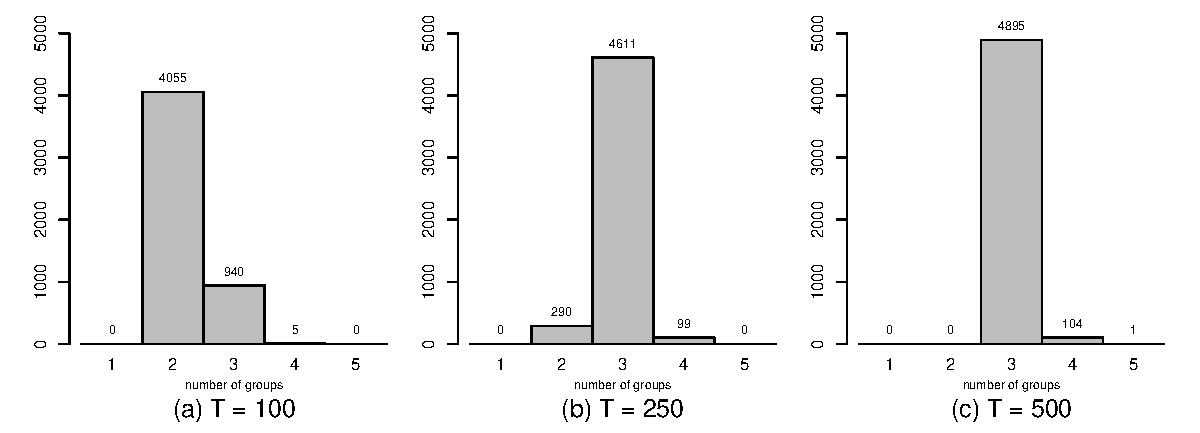
\includegraphics[width=\textwidth]{output/plots/sim/histograms_groups}
\caption{Estimated number of groups for nominal size $\alpha = 0.05$ and different sample sizes $T$. Each panel corresponds to a different sample size $T$.}
\label{fig:clustering:1}
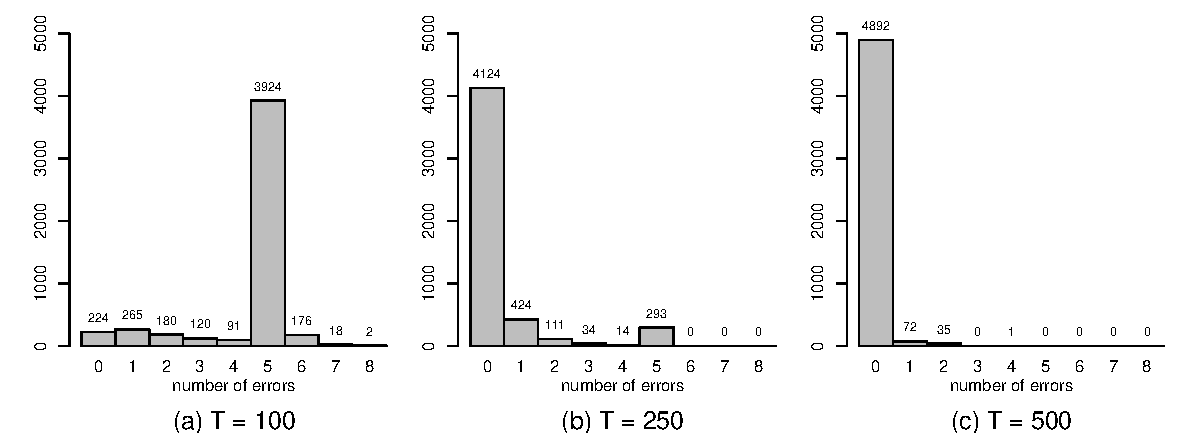
\includegraphics[width=\textwidth]{output/plots/sim/histograms_errors}
\caption{Number of incorrectly clustered time series for nominal size $\alpha = 0.05$ and different sample sizes $T$. Each panel corresponds to a different sample size $T$.}\label{fig:clustering:2}
\end{figure}

We finally investigate the finite sample performance of the clustering algorithm from Section \ref{sec:clustering}. To do so, we consider a very simple scenario: we generate data from the model $Y_{it} = m_i(\frac{t}{T}) + \varepsilon_{it}$, i.e., we assume that there are no fixed effects and no covariates influencing the data generating process. As before, we set the number of time series $i$ to $n = 15$ and we consider different time series lengths $T$. In order to introduce the group structure in the model, we partition the $n = 15$ time series into $N=3$ groups, each containing $5$ time series. Specifically, we set $G_1 = \{1,\ldots, 5\}$, $G_2 = \{6,\ldots, 10\}$ and $G_3 =  \{11,\ldots, 15\}$, and we assume that $m_i = f_l$ for all $i \in G_l$, $l = 1, 2, 3$. We define the group-specific trend functions $f_1$, $f_2$ and $f_3$ by $f_1(u) = 0$, $f_2(u) = 1 \cdot (u - 0.5)$ and $f_3(u) =  (- 1) \cdot (u - 0.5)$. In order to compute our estimators of the groups $G_1$, $G_2$, $G_3$ and their number $N = 3$, we use the same implementation as before followed by the clustering procedure from Section \ref{sec:clustering}. The estimation results are reported in Table \ref{tab:clustering} and Figures \ref{fig:clustering:1} and \ref{fig:clustering:2}. The entries in Table \ref{tab:clustering:1} are computed as the number of simulations for which $\widehat{N} = N$ divided by the total number of simulations. They thus specify the empirical probabilities with which the estimate $\widehat{N}$ is equal to the true number of groups $N = 3$. Analogously, the entries of Table \ref{tab:clustering:2} give the empirical probabilities with which the estimated group structure $\{ \widehat{G}_1,\ldots,\widehat{G}_{\widehat{N}}\}$ equals the true one $\{G_1,G_2,G_3\}$. In addition to the empirical probabilities provided in Table \ref{tab:clustering:1}, we depict histograms of the $S = 5000$ simulated values produced by an estimator $\hat{N}$ and of the number of mistakes that the clustering algorithm made in Figures \ref{fig:clustering:1} and \ref{fig:clustering:2}. The number of mistakes of the algorithm is equal to the number of incorrectly attributed time series and is calculated as 
$$\min_{\pi \in S_{\hat{N}}} |G_1 \setminus G_{\pi(1)}| +|G_2 \setminus G_{\pi(2)}| + |G_3 \setminus G_{\pi(3)}|,$$
where $S_{\hat{N}}$ is the set of all permutations of $\{1, 2, \ldots, \hat{N}\}$ and we assume that $G_{\pi(3)} = \emptyset$ in case $\hat{N} = 2$. The number of mistakes is equal to $0$ in case of $\{ \widehat{G}_1,\ldots,\widehat{G}_{\widehat{N}}\} = \{ G_1,G_2,G_3\}$ and in our simulation study, there were no cases of $9$ or more mistakes even for the smallest sample size $T = 100$.


The simulation results nicely illustrate the theoretical properties of our clustering algorithm. According to Proposition \ref{prop:clustering:1}, the probability that $\widehat{N} = N$ and $\{ \widehat{G}_1,\ldots,\widehat{G}_{\widehat{N}}\} = \{G_1,G_2,G_3\}$ should be at least $(1-\alpha)$ asymptotically. For the sample size $T = 500$, the empirical probabilities reported in Table \ref{tab:clustering} can indeed be seen to exceed the value $(1-\alpha)$ as predicted by Proposition \ref{prop:clustering:1}. %Only for $T = 500$ and $\alpha = 0.01$, the empirical probability is slightly below $(1-\alpha)$.
For the smaller sample sizes $T=100$ and $T=250$, in contrast, some of the empirical probabilities are much smaller than $(1-\alpha)$. This reflects the asymptotic nature of Proposition \ref{prop:clustering:1} and is not very surprising. It simply mirrors the fact that for small and moderate sample sizes, the effective noise level in the simulated data is quite high. Even though some of the empirical probabilities for $T=100$ and $T=250$ are clearly below the target $(1-\alpha)$, they are still quite substantial. Moreover, from Figures \ref{fig:clustering:1} and \ref{fig:clustering:2}, it is evident that for the smallest sample size $T =100$, our test underestimates the number of groups ($\widehat{N} = 2$ in $4055$ cases out of $5000$) and does not detect the difference between two out of three groups. This is also supported by the observation from Figure \ref{fig:clustering:2} that in $3924$ cases there are only $5$ mistakes made, hence, in most of these cases, the estimated group structure $\{ \widehat{G}_1, \widehat{G}_{2}\}$ coincides either with  $\{ G_1 \cup G_2,G_3\}$, or  $\{ G_1, G_2\cup G_3\}$, or $ \{ G_1 \cup G_3,G_2\}$. For moderate sample size $T = 250$, our estimates $\widehat{N}$ and $\{ \widehat{G}_1,\ldots,\widehat{G}_{\widehat{N}} \}$ are equal to the true values in a large number of simulations. 


\section{\textcolor{red}{Applications}}\label{sec:app}
\subsection{Analysis of the GDP growth}\label{subsec:app:gdp}


To illustrate our test method from Section \ref{sec:test}, we repeat an application example from \cite{Zhang2012} where the authors test the hypothesis of a common trend in the GDP growth data for $16$ OECD countries. Since we do not have access to the original dataset from \cite{Zhang2012} and to the exact data specifications the authors used in their paper, we perform our analysis on the data available from the common sources: Refinitiv Datastream, OECD.Stat database, Federal Reserve Economics Data (FRED) and Barro-Lee Educational Attainment dataset \citep*{Barro2013}. In our illustration example, we consider the specification of the data that is as close as possible to the one in \linebreak \cite{Zhang2012} with one important distinction. In the original study, the authors examine $16$ OECD countries (not specifying which ones), whereas we consider only $11$ countries\footnote{Australia, Austria, Canada, Finland, France, Germany, Japan, Norway, Switzerland, UK, and USA.} due to the availability of the data. The OECD.Stat database is the main source for the data on major economic indicators, and it contains  quarterly data of good quality covering the time period used in the original study only for $11$ countries used in our analysis. Similar data for other OECD countries in OECD.Stat database and in other notable sources contain many missing values. In the appendix, we repeat the analysis for aforementioned $11$ countries and additional $5$ countries using linear interpolation to impute the missing values in the data. Details how this interpolation is done are deferred to the Appendix.

We consider the same time period as in \cite{Zhang2012} from the fourth quarter of 1975 up to and including the third quarter of 2010. We collect the data from multiple sources. In the following list, we provide the specifications for the variables that we use in our analysis.

\begin{enumerate}
\item \textbf{GDP:} We use data on the Gross Domestic Product -- Expenditure Approach ($GDP$) from the OECD.Stat \nocite{OECD} database (https://stats.oecd.org/Index.aspx). The data are freely available and were accessed on 7 December 2021. To be as close as possible to the specification of the data in \cite{Zhang2012}, we use the seasonally adjusted quarterly data on the GDP expressed in millions of \linebreak 2015 US dollars.\footnote{Since the publication of the original paper in 2013, the OECD reference year has changed from 2005 to 2015. We have decided to analyse the latest version of the data in order to be able to make more accurate and up-to-date conclusions.} The data span from 1960 to 2021 which fully covers the analysed time period. 
%\item \textbf{Capital:} We use data on Capital Stock at Constant National Prices ($K$) from the Penn World Table \citep{Feenstra2015} retrieved from FRED \linebreak (https://fred.stlouisfed.org/, accessed on 7~December 2021). The data are given in the millions of the $2017$ US dollars. Since the observations are at an annual frequency, we linear interpolate the data to obtain the quarterly values. Our approach is different from the one in \cite{Zhang2012} where they use the quarterly data from the beginning. The reason for such discrepancy is the fact that we have not found the quarterly time series of sufficient quality on Capital Stock at Constant National Prices in the common sources. We repeat the analysis using the quarterly data on Gross Fixed Capital Formation instead of Capital Stock in the Appendix.
\item \textbf{Capital:} We use data on Gross Fixed Capital Formation ($K$) from the OECD.Stat \nocite{OECD} database (https://stats.oecd.org/Index.aspx). The data are freely available and were accessed on 7~December 2021. The values are at a quarterly frequency, seasonally adjusted, and expressed in the millions of the $2015$ US dollars. In contrast with \cite{Zhang2012}, where they use the data on Capital Stock at Constant National Prices, we choose to work with Gross Fixed Capital Formation due to the availability of the data. It is worth noting that since accurate data on capital stock is notoriously difficult to collect, the use of gross fixed capital formation as a measure of capital while explaining economic growth is standard in the literature (see, e.g., \cite{Sharma1994}, \cite{Lee2002}, \cite{Lee2005}).
\item \textbf{Labour:} We collect the data on the Number of Employed People ($L$) from various sources. For most of the countries (Austria, Australia, Canada, Germany, Japan, UK and the USA) we download the OECD data on Employed Population: Aged 15 and Over retrieved from FRED (https://fred.stlouisfed.org/, accessed on 7~December 2021). \nocite{OECDempl} The data for France and Switzerland were downloaded from Refinitiv Datastream on 7~December~2021. For all of the aforementioned countries the observations are at a quarterly frequency and seasonally adjusted. The data for Finland and Norway were also obtained via Refinitiv Datastream on 7~December~2021, however, the only quarterly time series that are long enough for our purposes are not seasonally adjusted. Hence, for these two countries we perform the seasonal adjustment ourselves. We do it using the default method of the function \verb|seas| from an \verb|R| package \verb|seasonal| \citep*{Sax2018} which is an interface to X-13-ARIMA-SEATS, the seasonal adjustment software used by the US Census Bureau. We repeat the analysis using not seasonally adjusted data for all of the $11$ countries as a robustness check and we report the results in the Appendix.

For all of the countries, the observations are given in thousands of persons.
\item \textbf{Human capital:} We use Educational Attainment for Population Aged 25 and Over ($H$) collected from http://www.barrolee.com (accessed on 7 December 2021) as a measure of human capital. Since the only available data is five-year census data, we follow \cite{Zhang2012} and use linear interpolation between the observations and constant extrapolation on the boundaries (second and third quarters of 2010) to obtain the quarterly time series.
\end{enumerate}


\begin{figure}[t]
\centering
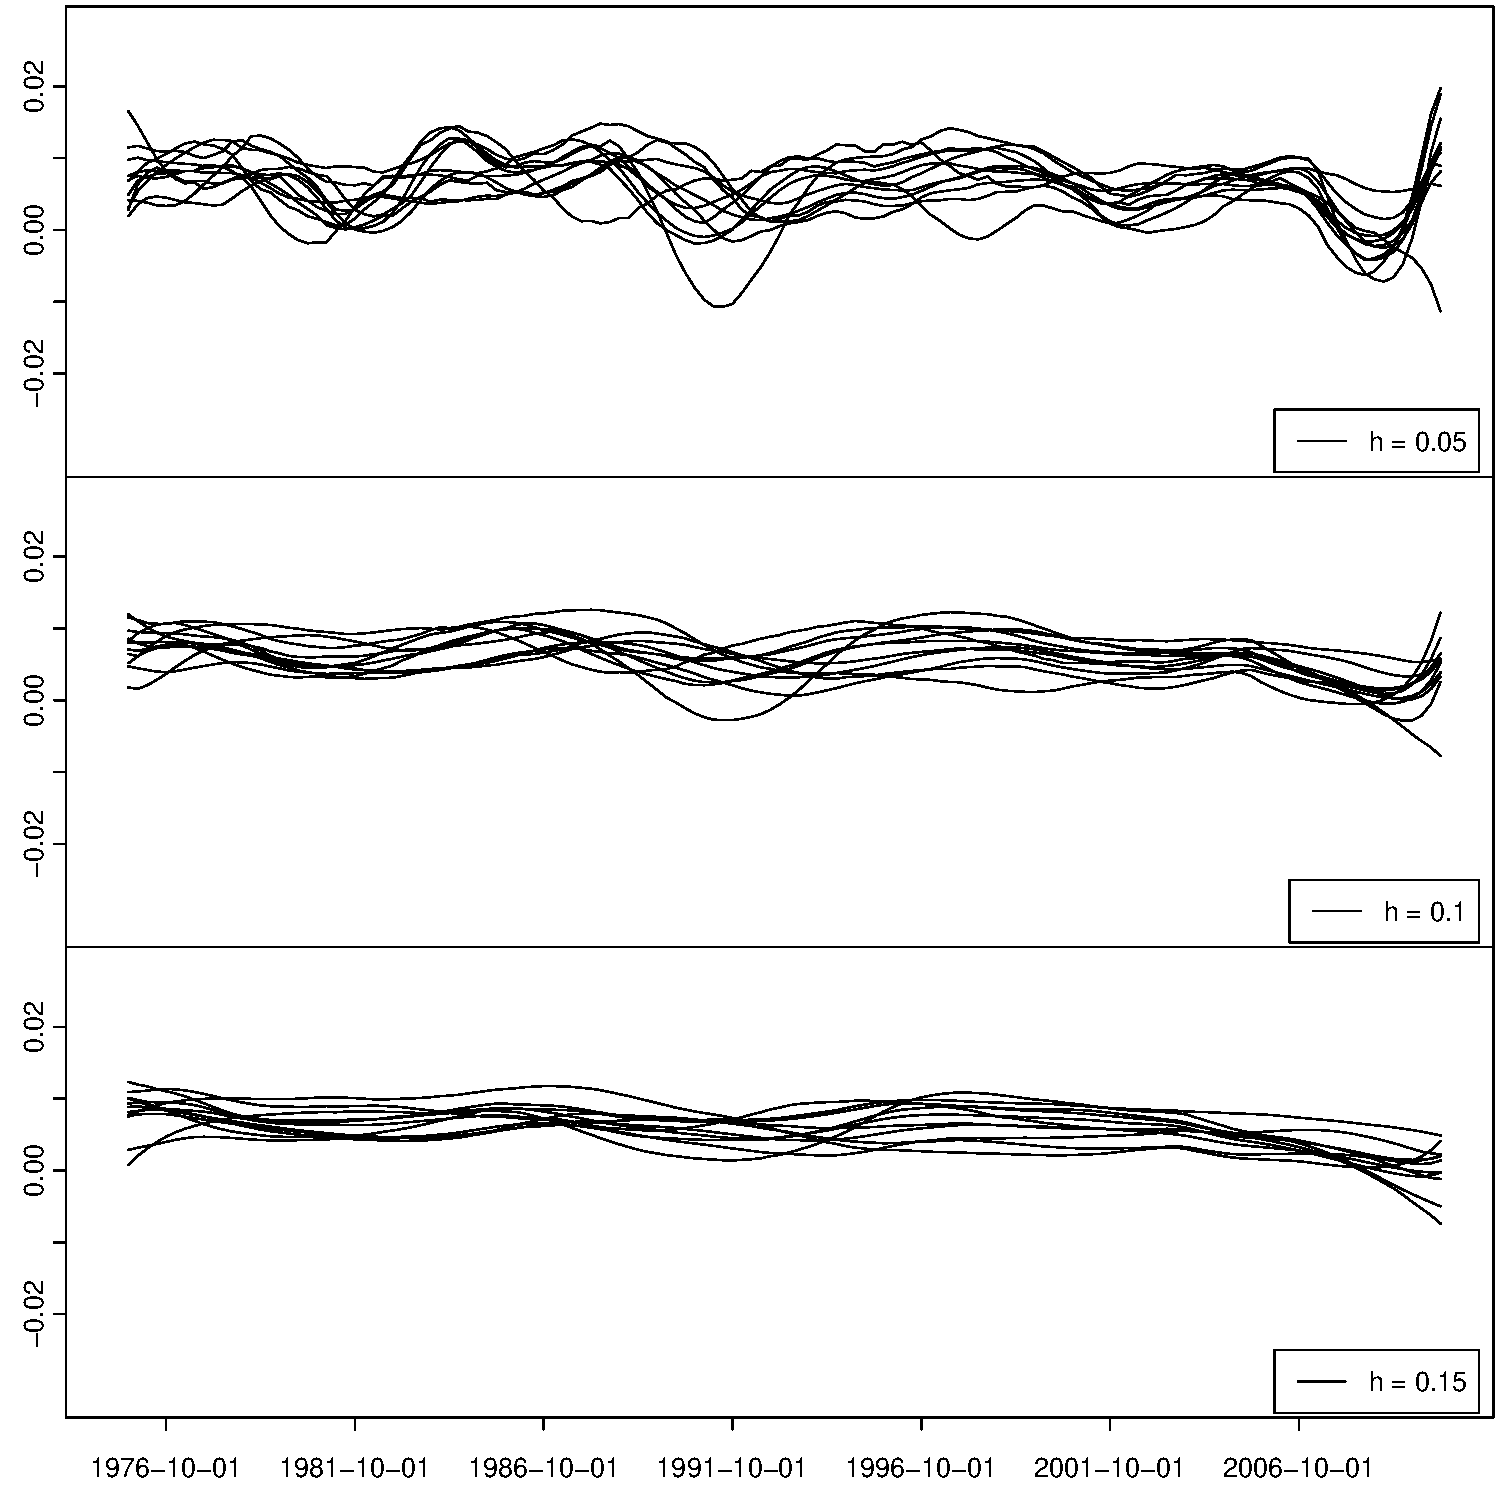
\includegraphics[width=0.8\textwidth]{output/plots/gdp/smoothed_gdp_data.pdf}
\vspace{0.2cm}
\caption{Local linear kernel estimates of the $n=11$ original time trends from the application of Section \ref{subsec:app:gdp}. Each panel shows the estimates for a different bandwidth $h$.}\label{fig:app:gdp}
\end{figure}

\begin{figure}[t]
\centering
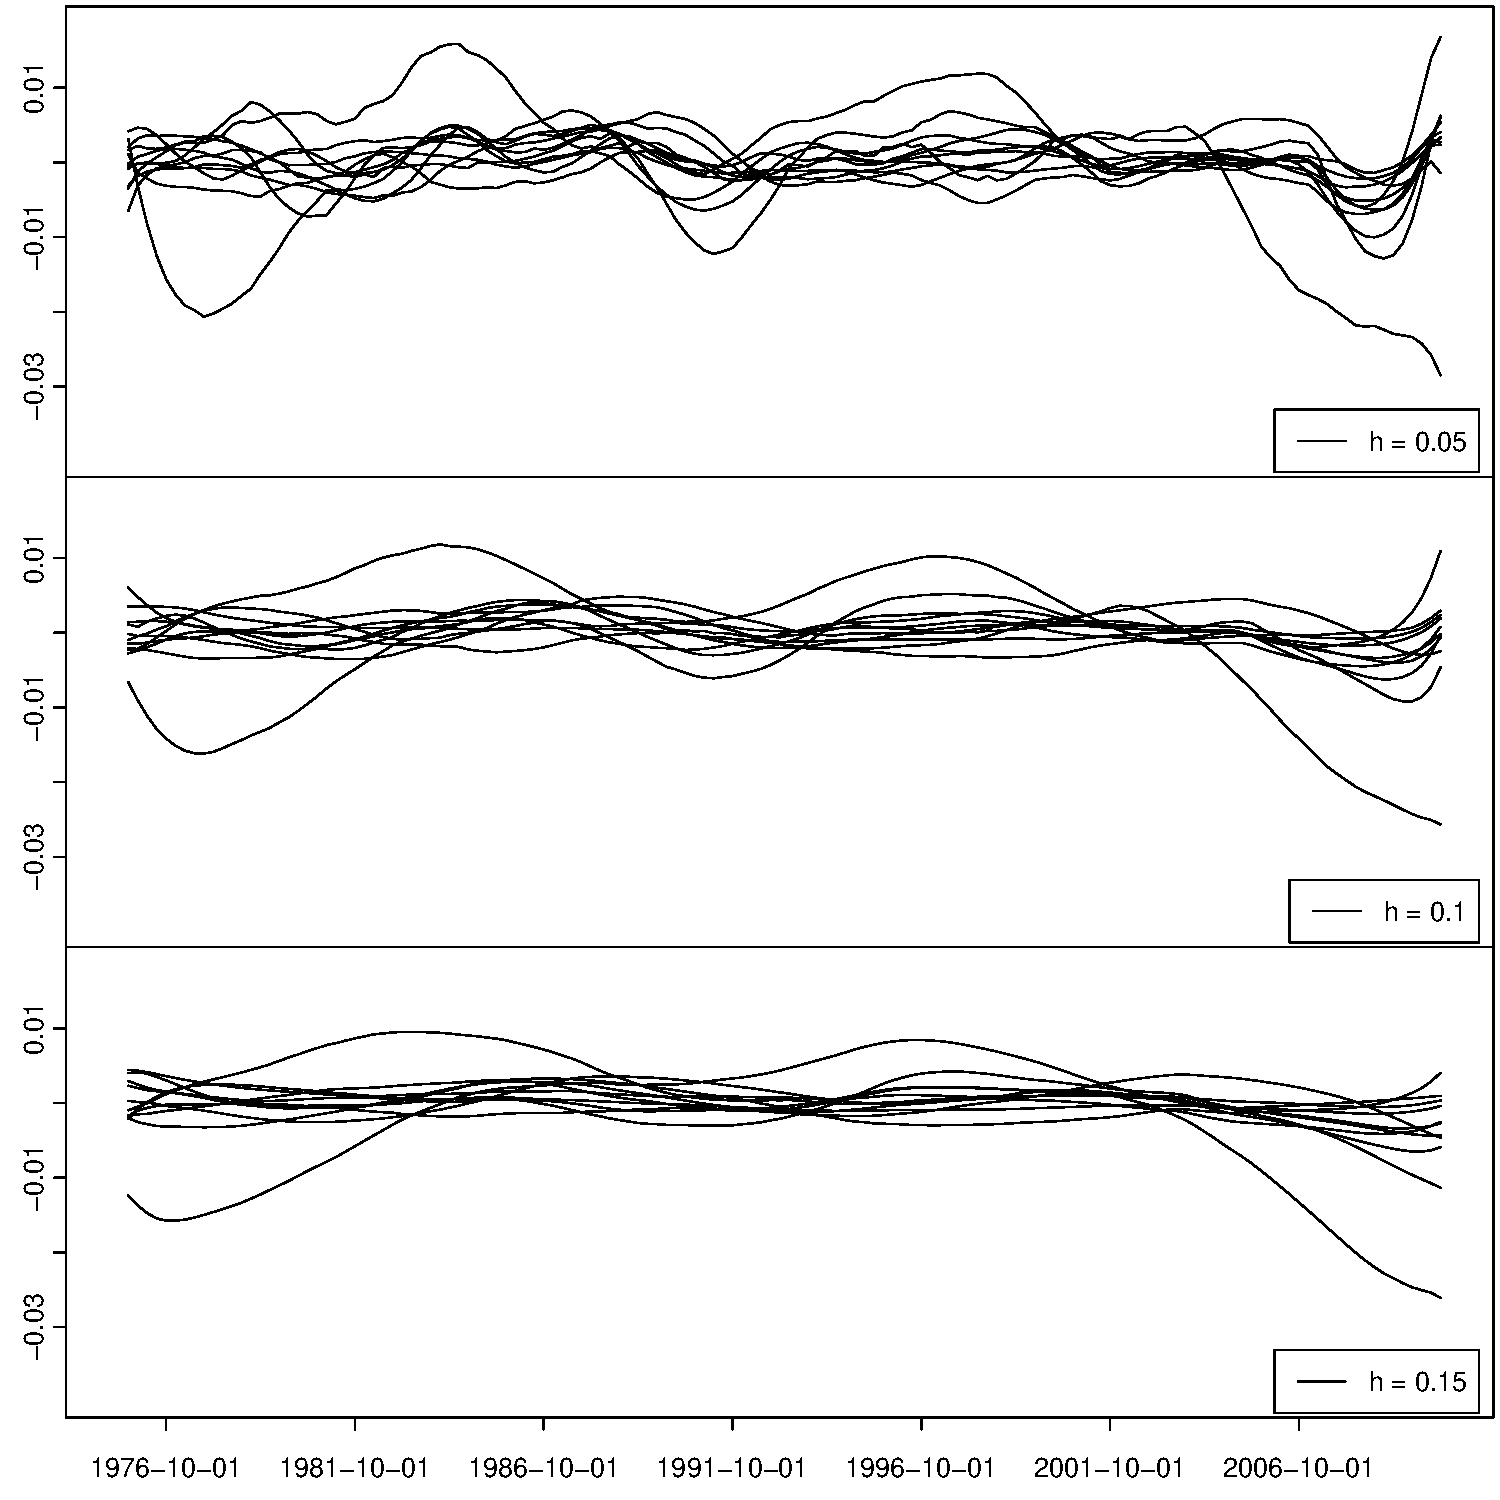
\includegraphics[width=0.8\textwidth]{output/plots/gdp/smoothed_gdp_data_augmented.pdf}
\vspace{0.2cm}
\caption{Local linear kernel estimates of the $n=11$ augmented time trends from the application of Section \ref{subsec:app:gdp}. Each panel shows the estimates for a different bandwidth $h$.}\label{fig:app:gdp_augm}
\end{figure}


We thus observe a panel of $n = 11$ time series $\mathcal{T}_i = \{(Y_{it}, \X_{it}): 1 \le t \le T \}$ of length $T = 140$ for each country $i \in \{1,\ldots, 11\}$, where $Y_{it} = \Delta \ln GDP_{it} := \ln GDP_{it} - \ln GDP_{i(t-1)}$, $\X_{it} = (\Delta \ln L_{it}, \Delta \ln K_{it}, \Delta \ln H_{it})^\top$ with $\Delta \ln L_{it} := \ln L_{it} - \ln L_{i(t-1)}$, $\Delta \ln K_{it} := \ln K_{it} - \ln K_{i(t-1)}$ and $\Delta \ln H_{it} := \ln H_{it} - \ln H_{i(t-1)}$. Without loss of generality, we let $\Delta \ln GDP_{i1} = \Delta \ln L_{i1} = \Delta \ln K_{i1} = \Delta \ln H_{i1} = 0$. The time series $\mathcal{T}_i$ is assumed to follow the model 
\begin{equation}\label{eq:model:app}
Y_{it} = \bfbeta^\top_i \X_{it} + m_i \Big( \frac{t}{T} \Big) + \alpha_i + \varepsilon_{it} 
\end{equation}
for $1 \le t \le T$, where $\bfbeta_i = (\beta_{i, 1}, \beta_{i, 2}, \beta_{i, 3})^\top$ is a vector of unknown parameters, $m_i$ is a country-specific unknown nonparametric time trend, and $\alpha_i$ is a fixed-effect term. Similarly to \cite{Zhang2012}, we rewrite the model \eqref{eq:model:app} as
\begin{equation}\label{eq:model:app2}
\Delta \ln GDP_{it} = \beta_{i, 1} \Delta \ln L_{it} + \beta_{i, 2} \Delta \ln K_{it} + \beta_{i, 3} \Delta \ln H_{it} + m_i \Big( \frac{t}{T} \Big) + \alpha_i + \varepsilon_{it},
\end{equation}

for $i \in \{1, \ldots, 11\}$ and $t \in \{1, \ldots, 140\}$.

Our test procedure depends on the estimator of the long-run variance $\sigma_i^2$ for the error process $\mathcal{E}_i = \{\varepsilon_{it}: 1 \le t \le T\}$. As was mentioned in Section \ref{subsec:test:prep}, without imposing any assumptions on the error terms, the estimator tends to be imprecise. To improve the behaviour of the estimator in a finite sample, we decide for imposing a certain time series structure on the error process in our analysis. Specifically, we assume that for each $i$ the error process $\mathcal{E}_i$ follows an AR($p_i$) model $\varepsilon_{it} = \sum_{j=1}^{p_i} a_{i, j} \varepsilon_{i(t-j)} + \eta_{it}$, where the order of the process $p_i$ is country-specific and not known and $\eta_{it}$ are i.i.d.\ innovations with mean zero. We choose $p_i$ as the minimiser of the Bayesian Information Criterion (BIC).\footnote{We also calculate the values of other information criteria such as FPE, AIC and HQ which, in most of the cases, resulted in the same values of $p_i$.} This yields $p_i = 3$ for Australia, Canada and the UK, and $p_i = 1$ for all other countries. This assumption allows us to use a difference-based long-run variance estimator proposed in \cite{KhismatullinaVogt2020}.% with the choice of the tuning parameters described below.

We aim to test whether the time trend $m_i$ is the same for all $11$ countries. In other words, we want to test the null hypothesis $H_0: m_1 = \ldots = m_n$ with $n = 11$ in model \eqref{eq:model:app2}. To do so, we implement the multiscale test from Section \ref{sec:test} in the following way. 
\begin{enumerate}
\item We choose $K$ to be an Epanechnikov kernel.
\item We let $\mathcal{G}_T = U_T \times H_T$ with 
\begin{align*}
U_T & = \big\{ u \in [0,1]: u = \textstyle{\frac{8t + 1}{2T}} \text{ for some } t \in \naturals \big\} \\
H_T & = \big\{ h \in \big[ \textstyle{\frac{\log T}{T}}, \textstyle{\frac{1}{4}} \big]:  h = \textstyle{\frac{4t}{T}} \text{ for some } t \in \naturals \big\}. 
\end{align*}
We thus take into account all locations $u$ on an equidistant grid $U_T$ with step length $4/T$ and all bandwidths $h=4/T, 8/T, 12/T,\ldots$ with $\log T /T \le h \le 1/4$. Note that $\mathcal{G}_T$ is not a subset of $\mathcal{G}_T^{\text{full}}$ since we do not assume that the considered locations take the form of $u = t/T$ for some $1 \leq t \leq T$. In our case, the choice of the grid $U_T$ is motivated by the structure of the data: for each interval $\mathcal{I}_{(u, h)} = [u-h, u+h]$, the effective sample size is $8, 16, 24, \ldots$ quarters, i.e. $2, 4, 6, \ldots$ years. It can be shown that with this choice of the grid the theoretical properties of our method remain the same. Furthermore, the lower bound $\log T / T$ is explained by Assumption \ref{C-h} which requires that $\log T /T \ll h_{\min}$ (given that all moments of $\varepsilon_{it}$ exist).
\item We estimate the unknown parameters $\bfbeta_i = (\beta_{i, 1}, \beta_{i, 2}, \beta_{i, 3})^\top$ for each country $i$ separately using the first-differencing approach described in Section \ref{subsec:test:prep}.
\item We compute the estimator of the fixed-effect term $\alpha_i$ by employing \eqref{eq:alpha:est}. We then work with the augmented time series $\widehat{Y}_{it} = Y_{it} - \widehat{\bfbeta}_i^\top \X_{it} - \widehat{\alpha}_{i}$ instead of the original data on the GDP growth rate $Y_{it}$.
\item To obtain the estimator $\hat{\sigma}_i^2$ of the long-run error variance $\sigma^2_i$, for each $i$ we apply the procedure from \cite{KhismatullinaVogt2020} to the augmented values \linebreak $\{\widehat{Y}_{it}: 1\leq t \leq T\}$. The details are summarised in Section \ref{subsec:app:lrv} of the Appendix. % with the following specification of the parameters: $\underline{r}=1$, $\overline{r}=10$ and $q = 15$.
We use $\hat{\sigma}^2_i$ for calculating the value of our main test statistic $\widehat{\Psi}_{n, T}$. %In the Appendix, we repeat the analysis using the averaged estimator $\hat{\sigma}^2 = \frac{1}{n}\sum_{i=1}^n \hat{\sigma}_i^2$.
%\item The significance levels are taken to be $\alpha = 0.05$ and $\alpha = 0.1$ (\citet{Zhang2012} report the results for testing at a significance level $\alpha = 0.1$).
\item To obtain the (approximate) critical values $q_{n, T}(\alpha)$ of the multiscale test, we simulate $5000$ values of the statistic $\Phi_{n, T}$ defined in Section \ref{subsec:test:test} and compute their empirical $(1-\alpha)$ quantile $\hat{q}_{n, T}(\alpha)$.
\end{enumerate}

 %We implement the test in the same way as in the simulations of Section \ref{sec:sim}. 


Figure \ref{fig:app:gdp} depicts smoothed version of the original time series on the GDP growth rate $\{Y_{it} = \Delta \ln GDP_{it}: 1 \le t \le T\}$ for each country $i$ of the $n=11$ countries under consideration. Figure \ref{fig:app:gdp_augm} presents local linear estimates of the trend functions $m_i$ for these countries after factoring out the effects of the covariates and the fixed-effect terms (i.e. calculated from the augmented time series~$\widehat{Y}_{it}$). In both figures, each panel corresponds to a different value of the bandwidth~$h$.

As can be seen in Figure \ref{fig:app:gdp}, in the original data on the GDP growth there are some notable differences between the countries for bandwidths $h = 0.05$ and $h = 0.1$. For example, while most of the countries experience the increase in the growth rate in the last two years, the data for one of the countries (Norway) suggests a decrease in the same period of time. Moreover, using the smallest bandwidth ($h= 0.05$) allows us to notice considerable differences in the behaviour of the time series in the middle of our time region. In contrast, the value of the bandwidth $h = 0.15$ is too big to detect any heterogeneity in the behaviour of the trends. As we see, the choice of the bandwidth is crucial in making conclusions in this example.

\begin{figure}[b!]
\begin{minipage}[t]{0.49\textwidth}
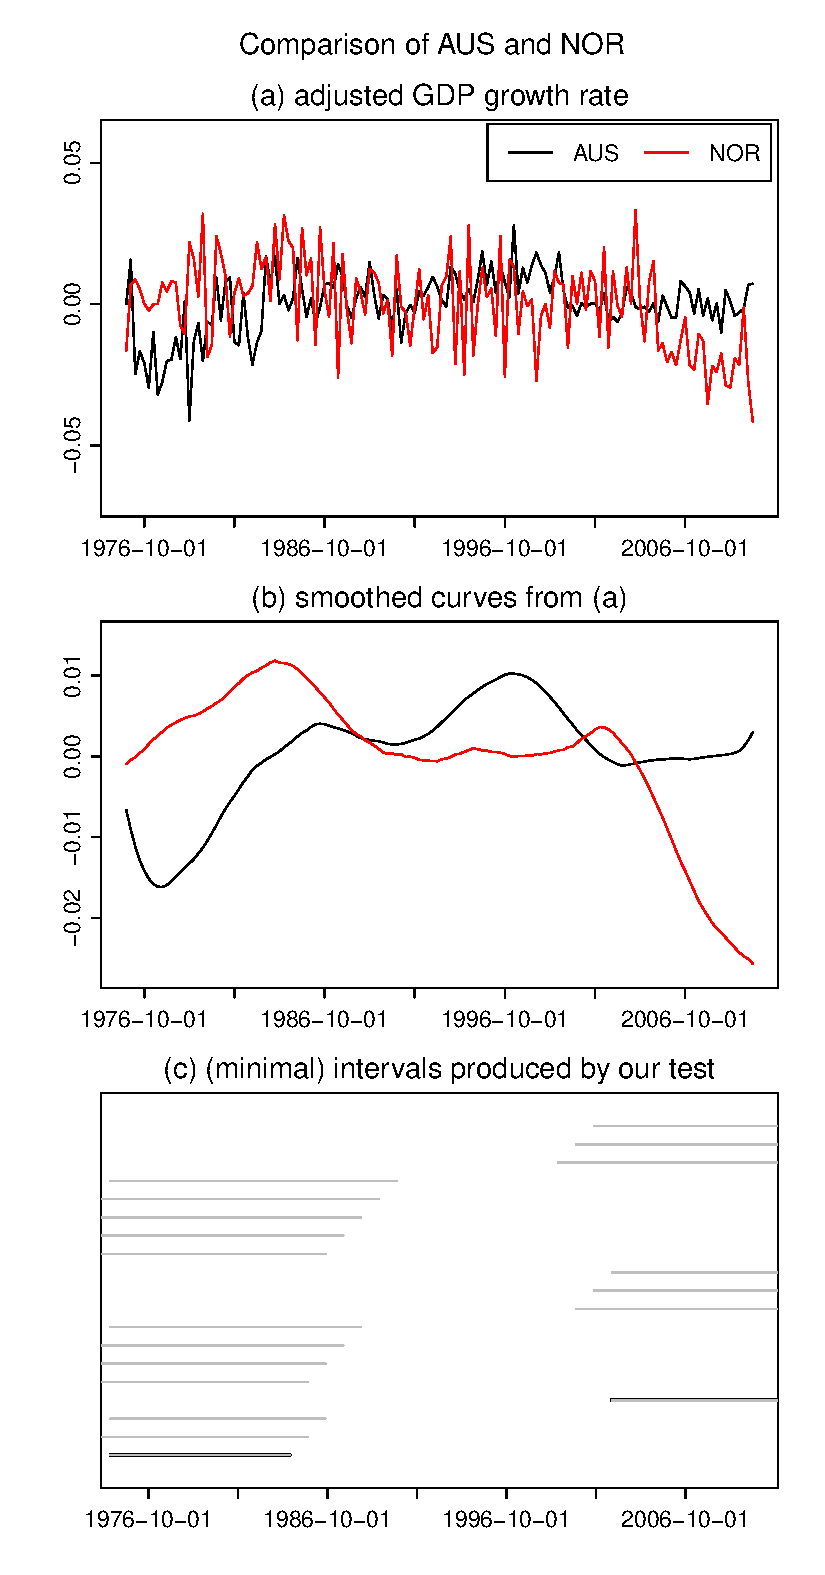
\includegraphics[width=\textwidth]{output/plots/gdp/AUS_vs_NOR}
\caption{Test results for the comparison of Australia and Norway.}\label{fig:Australia:Norway}
\end{minipage}
\hspace{0.25cm}
\begin{minipage}[t]{0.49\textwidth}
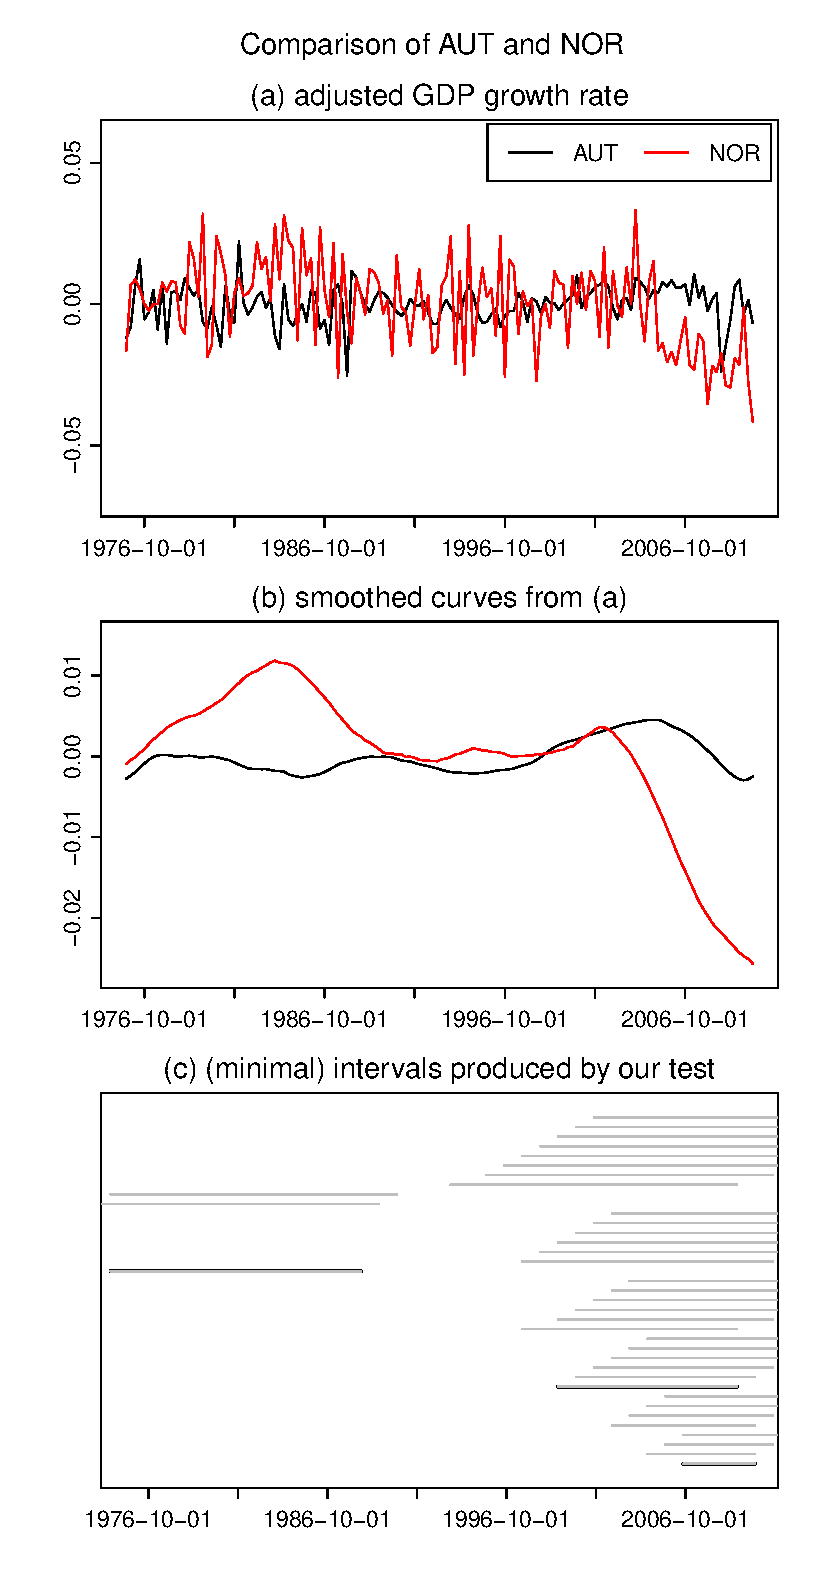
\includegraphics[width=\textwidth]{output/plots/gdp/AUT_vs_NOR}
\caption{Test results for the comparison of Austria and Norway.}\label{fig:Austria:Norway}
\end{minipage}
\caption*{Note: In each figure, panel (a) shows the two augmented time series, panel (b) presents smoothed versions of the augmented time series, and panel (c) depicts the set of intervals $\mathcal{S}^{[i, j]}(\alpha)$ in grey and the subset of minimal intervals $\mathcal{S}^{[i, j]}_{min}(\alpha)$ in black.}
\end{figure}

\begin{figure}[t!]
\begin{minipage}[t]{0.49\textwidth}
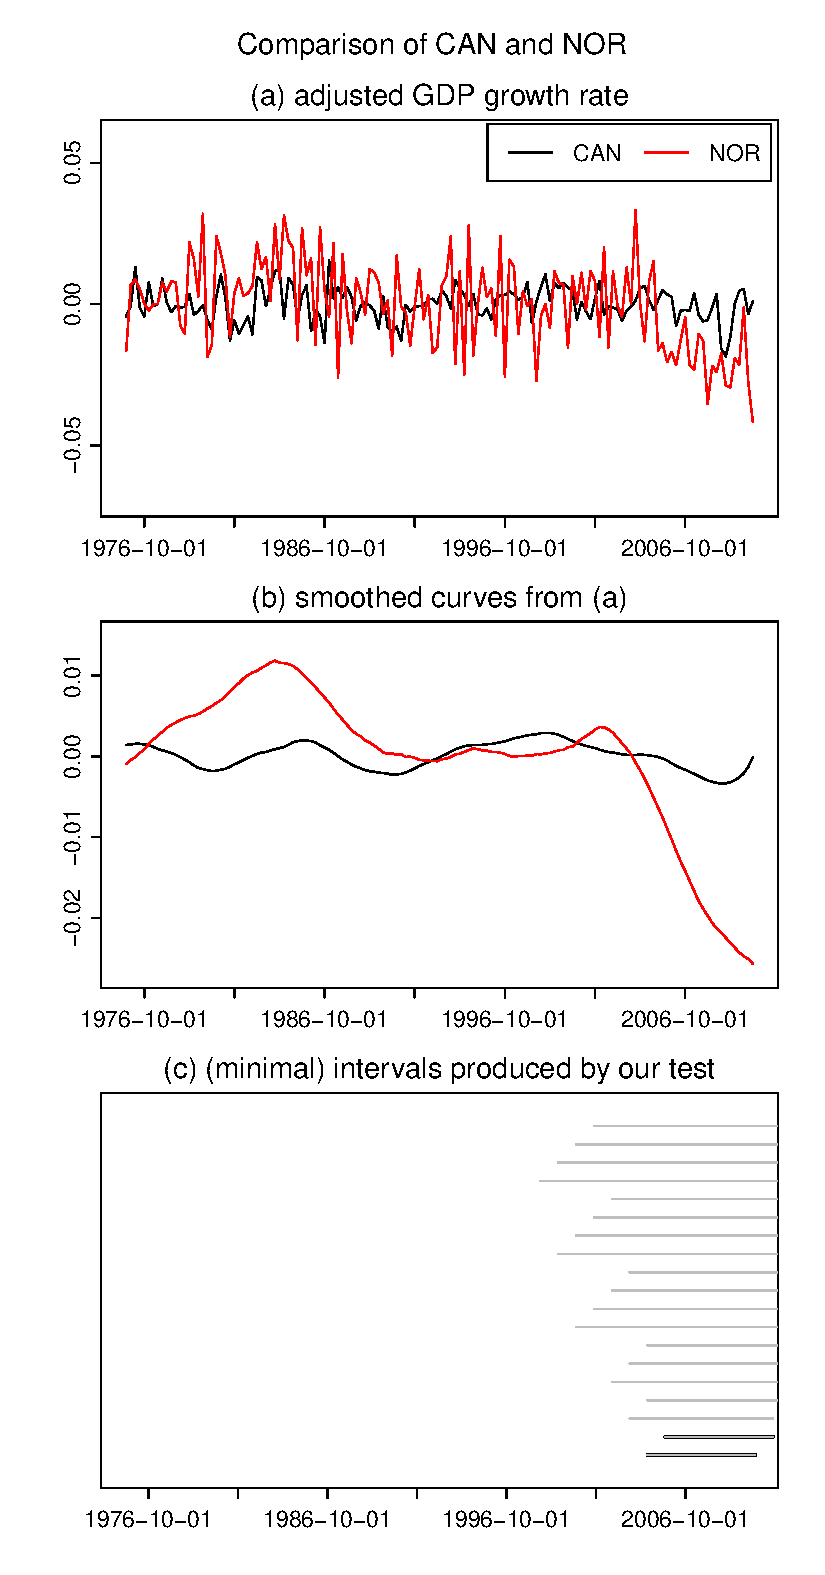
\includegraphics[width=\textwidth]{output/plots/gdp/CAN_vs_NOR}
\caption{Test results for the comparison of Canada and Norway.}\label{fig:Canada:Norway}
\end{minipage}
\hspace{0.25cm}
\begin{minipage}[t]{0.49\textwidth}
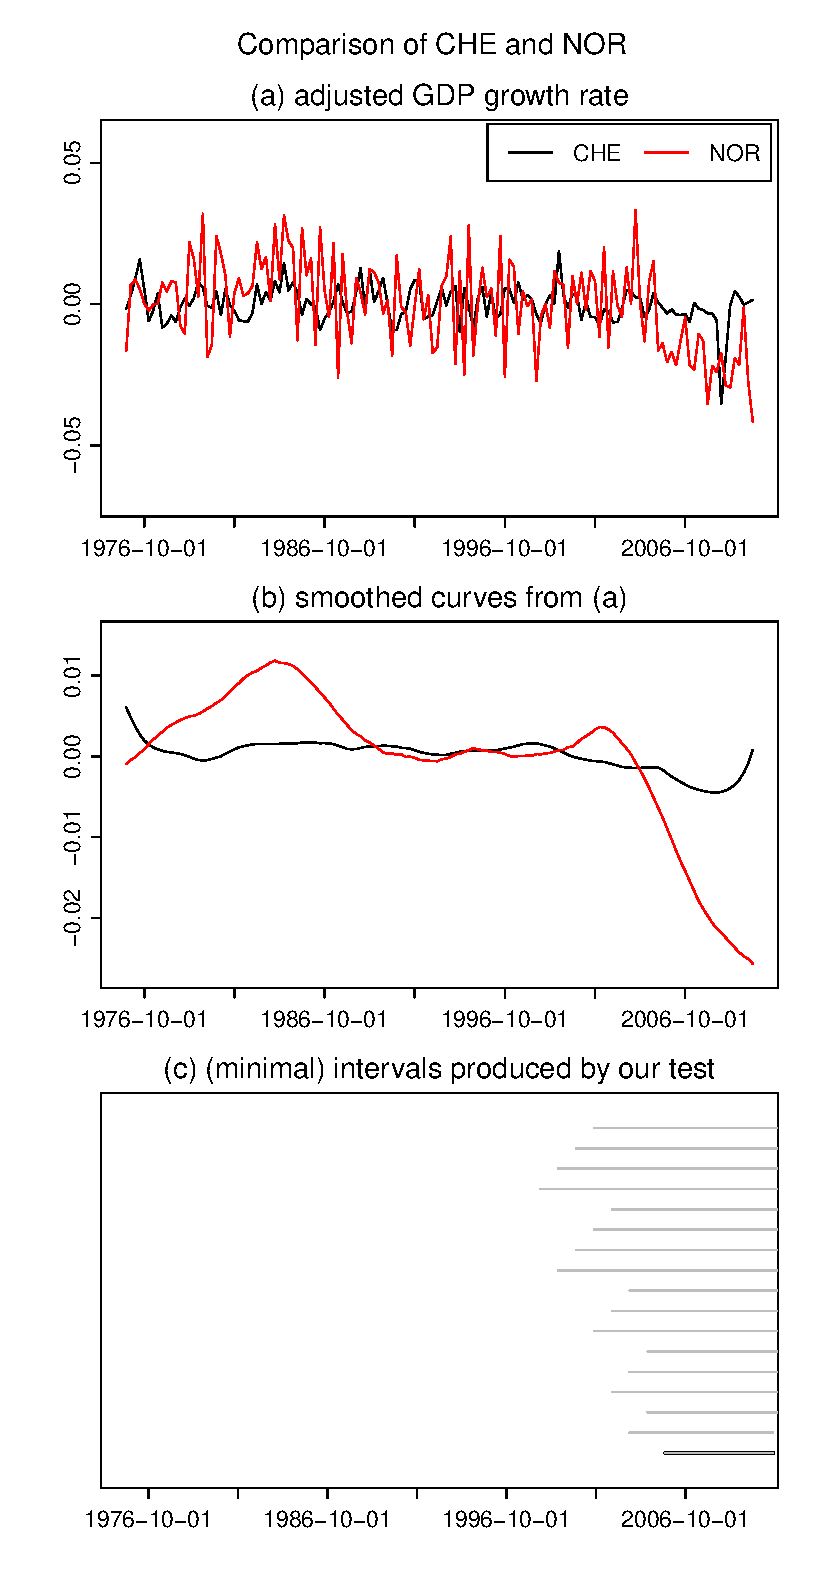
\includegraphics[width=\textwidth]{output/plots/gdp/CHE_vs_NOR}
\caption{Test results for the comparison of Switzerland and Norway.}\label{fig:Switzerland:Norway}
\end{minipage}
\caption*{Note: In each figure, panel (a) shows the two augmented time series, panel (b) presents smoothed versions of the augmented time series, and panel (c) depicts the set of intervals $\mathcal{S}^{[i, j]}(\alpha)$ in grey and the subset of minimal intervals $\mathcal{S}^{[i, j]}_{min}(\alpha)$ in black.}
\end{figure}

\begin{figure}[t!]
\begin{minipage}[t]{0.49\textwidth}
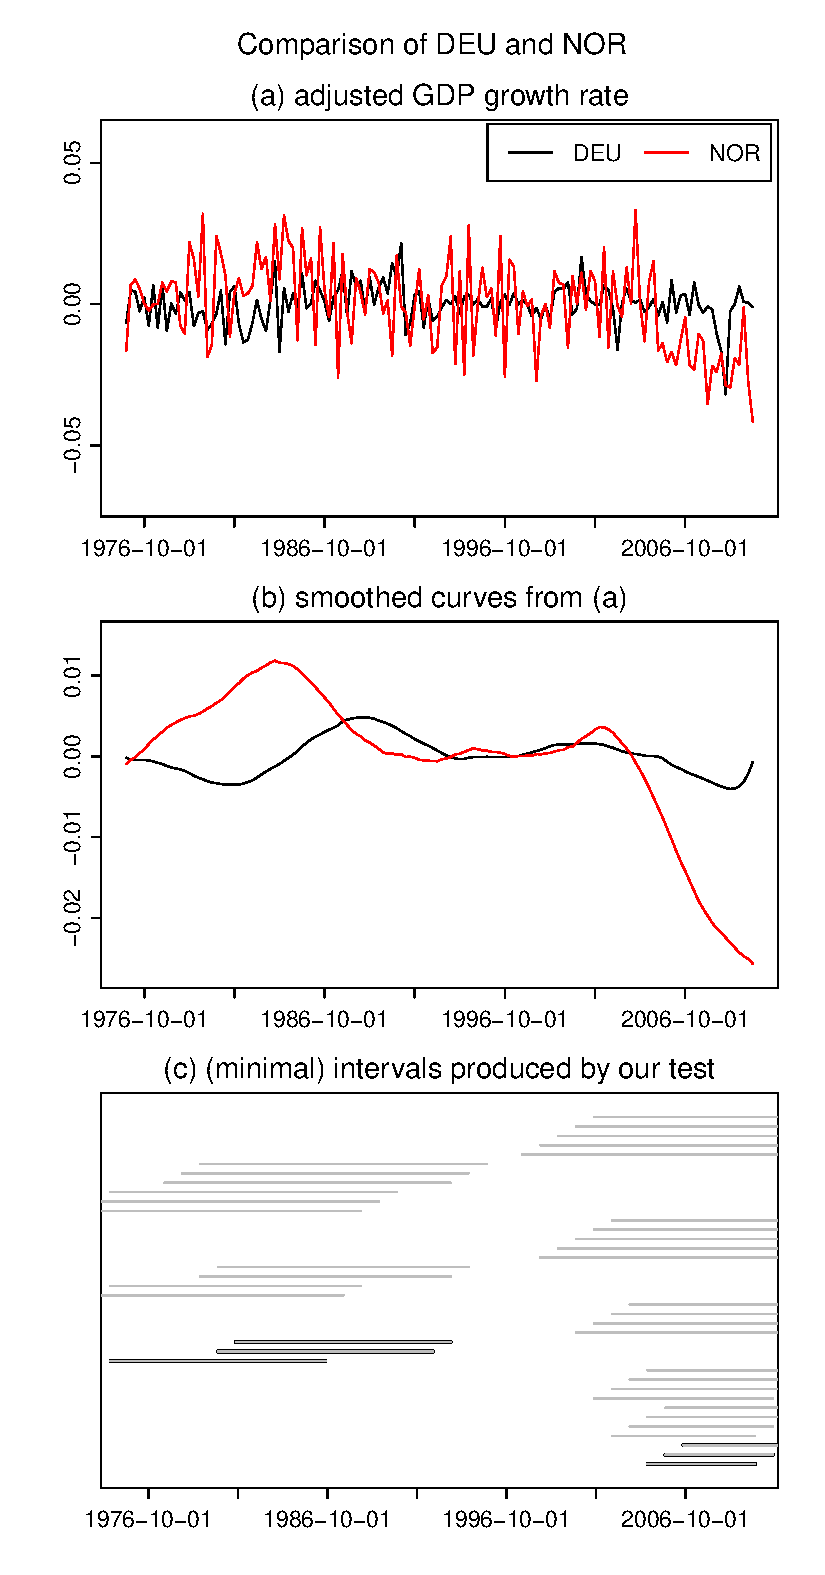
\includegraphics[width=\textwidth]{output/plots/gdp/DEU_vs_NOR}
\caption{Test results for the comparison of Germany and Norway.}\label{fig:Germany:Norway}
\end{minipage}
\hspace{0.25cm}
\begin{minipage}[t]{0.49\textwidth}
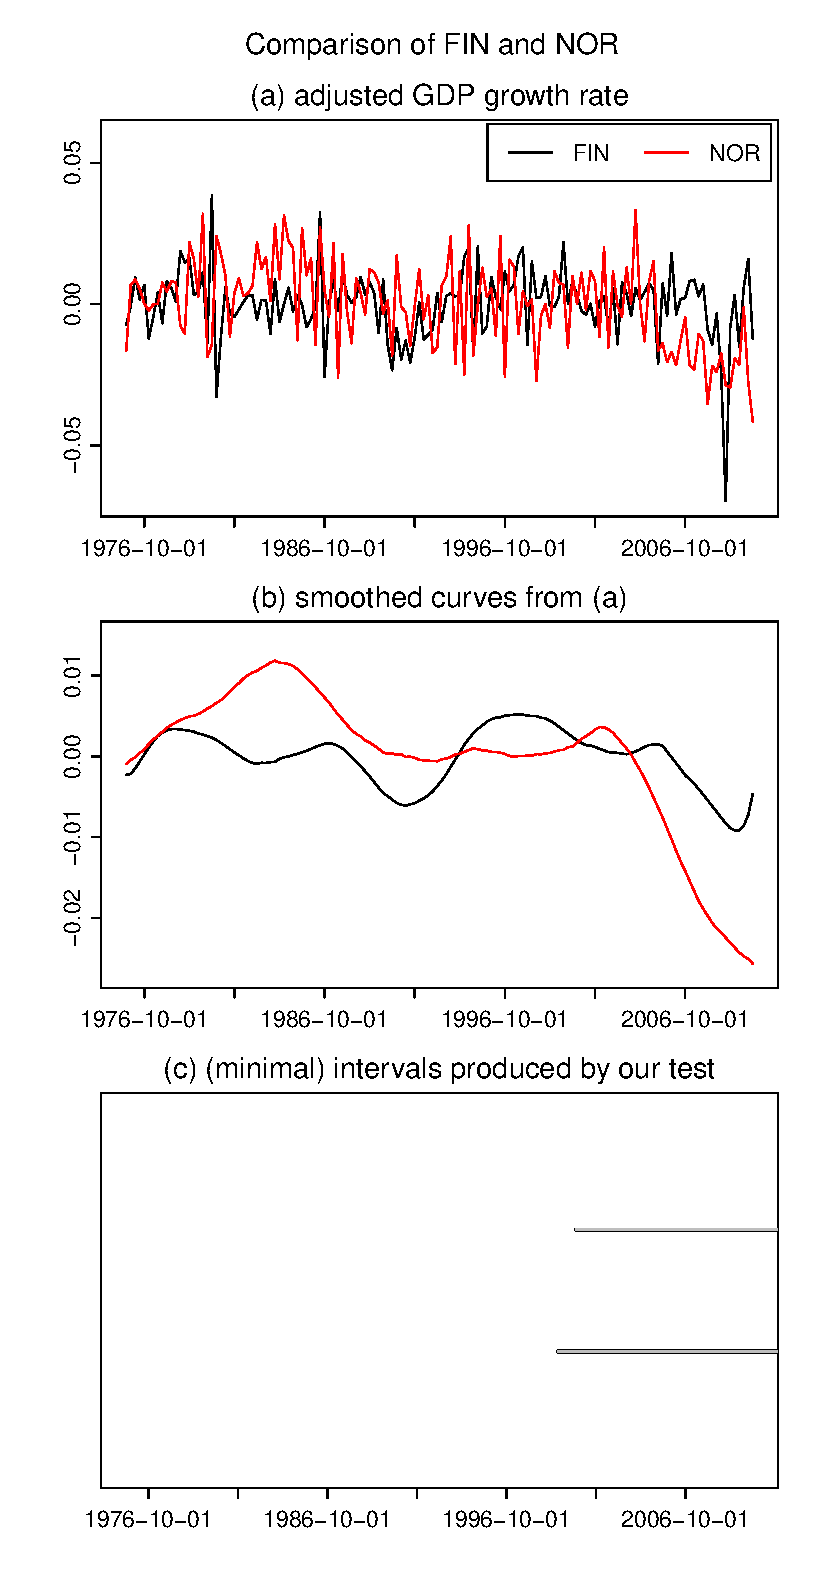
\includegraphics[width=\textwidth]{output/plots/gdp/FIN_vs_NOR}
\caption{Test results for the comparison of Finland and Norway.}\label{fig:Finland:Norway}
\end{minipage}
\caption*{Note: In each figure, panel (a) shows the two augmented time series, panel (b) presents smoothed versions of the augmented time series, and panel (c) depicts the set of intervals $\mathcal{S}^{[i, j]}(\alpha)$ in grey and the subset of minimal intervals $\mathcal{S}^{[i, j]}_{min}(\alpha)$ in black.}
\end{figure}

\begin{figure}[t!]
\begin{minipage}[t]{0.49\textwidth}
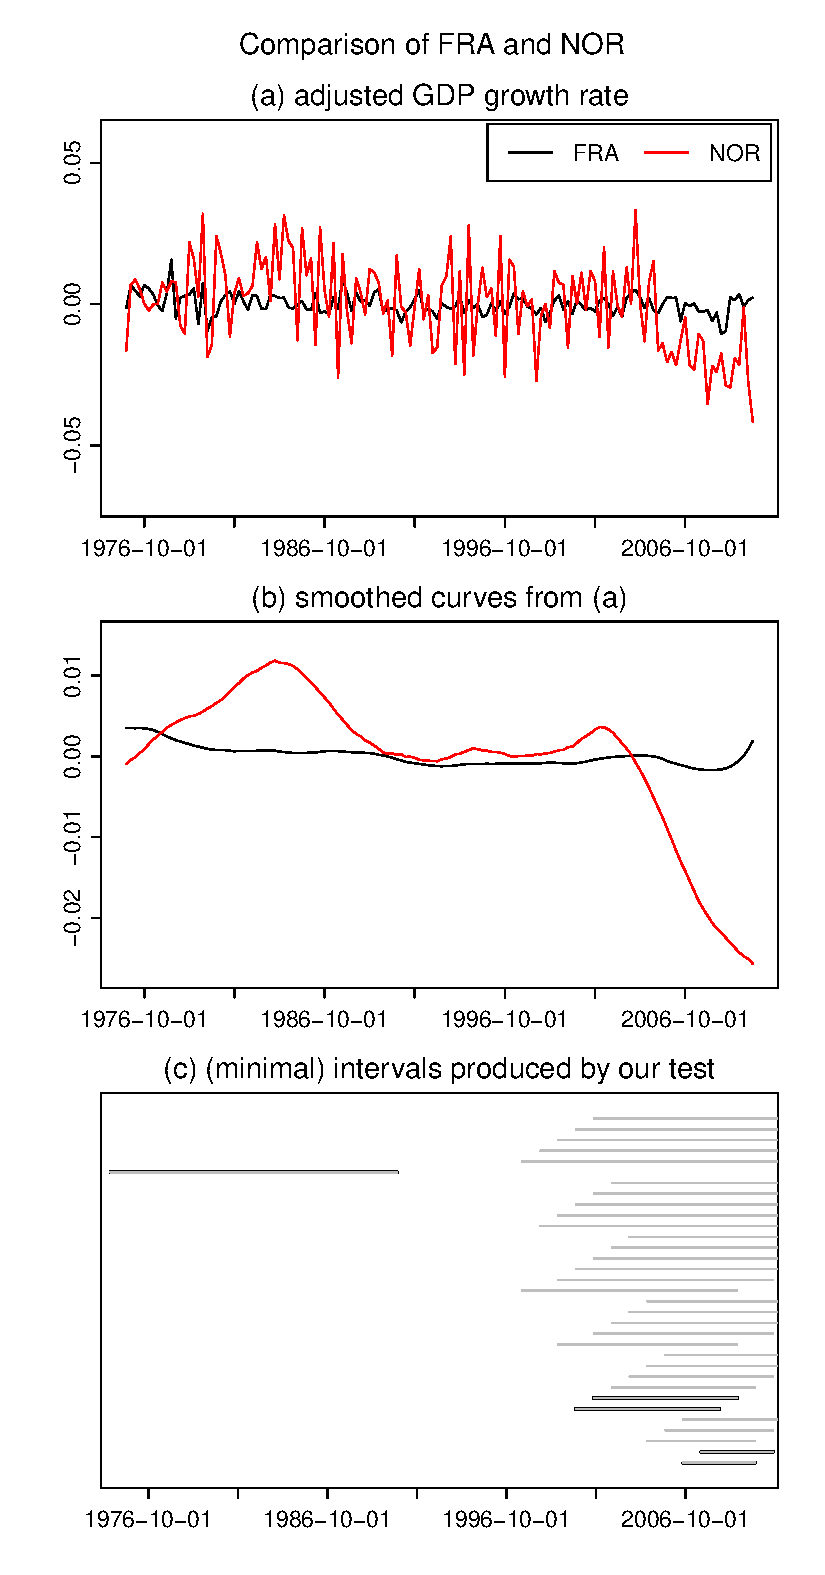
\includegraphics[width=\textwidth]{output/plots/gdp/FRA_vs_NOR}
\caption{Test results for the comparison of France and Norway.}\label{fig:France:Norway}
\end{minipage}
\hspace{0.25cm}
\begin{minipage}[t]{0.49\textwidth}
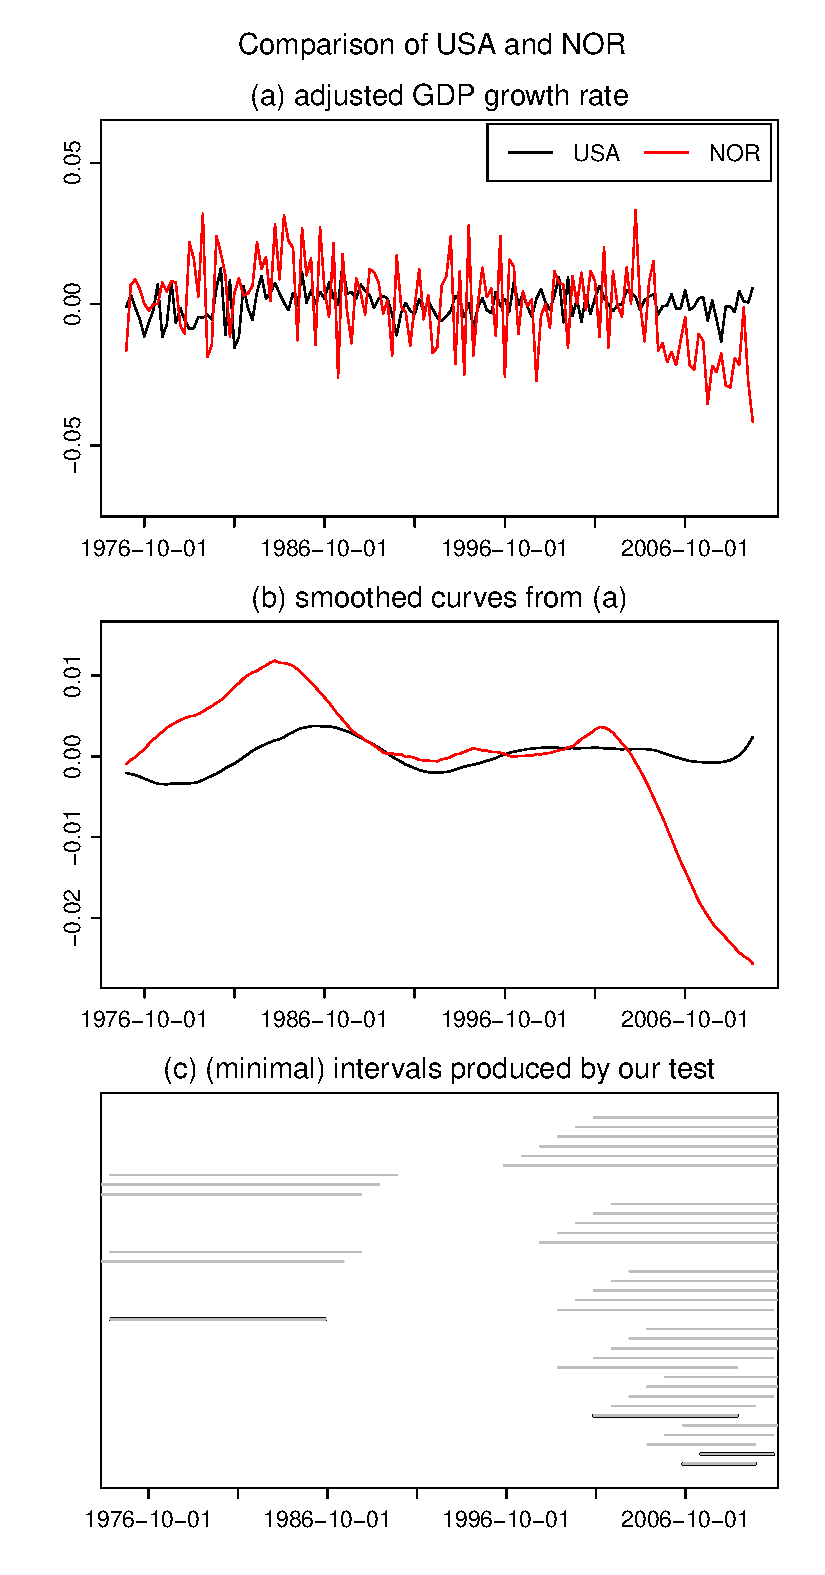
\includegraphics[width=\textwidth]{output/plots/gdp/USA_vs_NOR}
\caption{Test results for the comparison of the USA and Norway.}\label{fig:USA:Norway}
\end{minipage}
\caption*{Note: In each figure, panel (a) shows the two augmented time series, panel (b) presents smoothed versions of the augmented time series, and panel (c) depicts the set of intervals $\mathcal{S}^{[i, j]}(\alpha)$ in grey and the subset of minimal intervals $\mathcal{S}^{[i, j]}_{min}(\alpha)$ in black.}
\end{figure}

\begin{figure}[p!]
\begin{center}
\begin{minipage}[t]{0.49\textwidth}
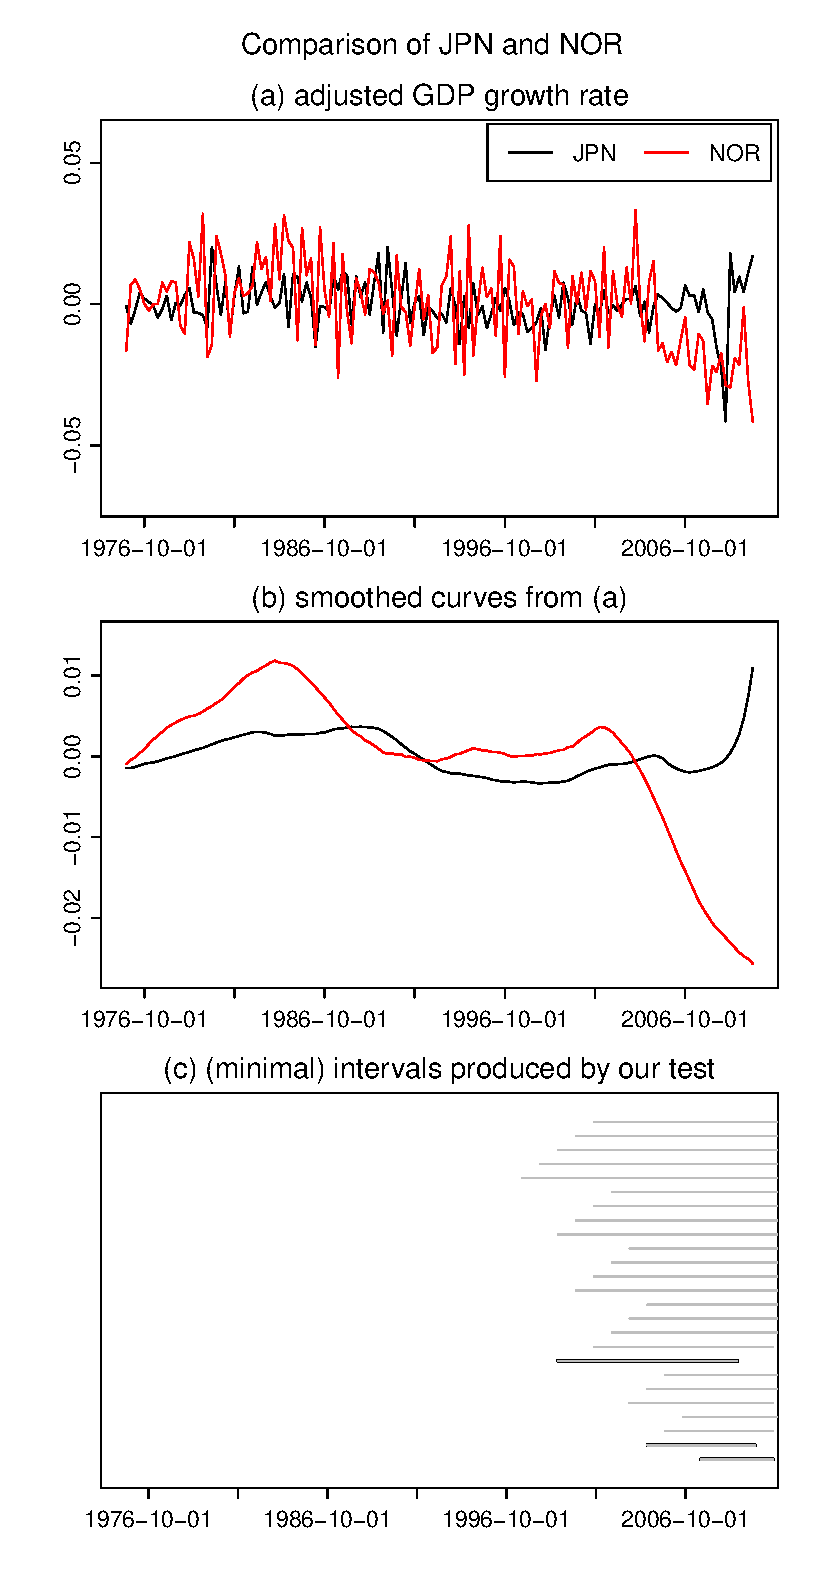
\includegraphics[width=\textwidth]{output/plots/gdp/JPN_vs_NOR}
\caption{Test results for the comparison of Japan and Norway.}\label{fig:Japan:Norway}
\end{minipage}
\end{center}
\caption*{Note: Panel (a) shows the two augmented time series, panel (b) presents smoothed versions of the augmented time series, and panel (c) depicts the set of intervals $\mathcal{S}^{[i, j]}(\alpha)$ in grey and the subset of minimal intervals $\mathcal{S}^{[i, j]}_{min}(\alpha)$ in black.}
\end{figure}


\begin{figure}[p!]
\begin{minipage}[t]{0.49\textwidth}
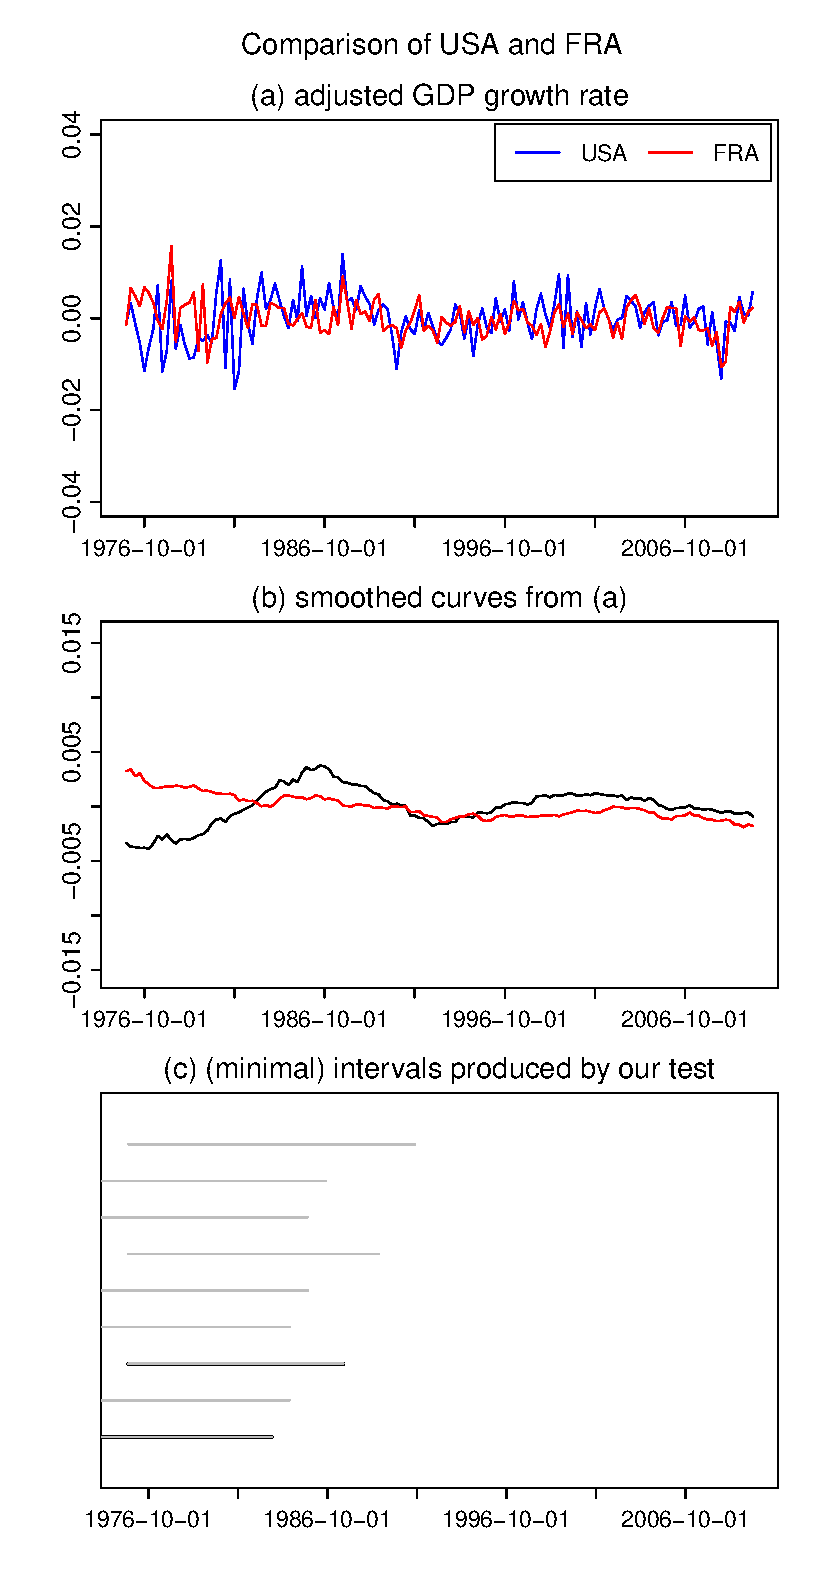
\includegraphics[width=\textwidth]{output/plots/gdp/USA_vs_FRA}
\caption{Test results for the comparison of the USA and France.}\label{fig:USA:France}
\end{minipage}
\hspace{0.25cm}
\begin{minipage}[t]{0.49\textwidth}
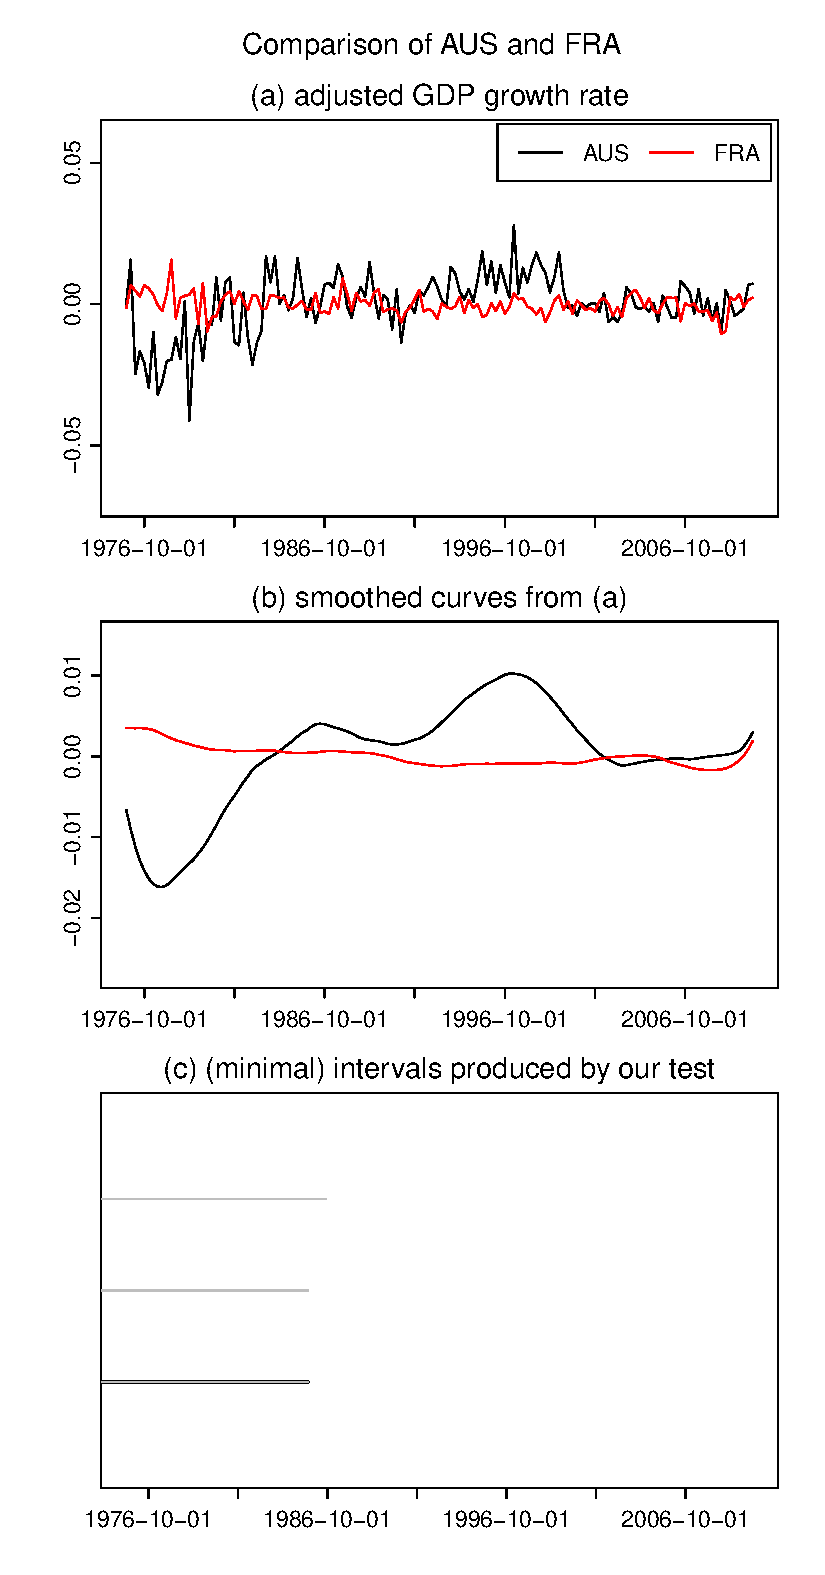
\includegraphics[width=\textwidth]{output/plots/gdp/AUS_vs_FRA}
\caption{Test results for the comparison of Australia and France.}\label{fig:Australia:France}
\end{minipage}
\caption*{Note: In each figure, panel (a) shows the two augmented time series, panel (b) presents smoothed versions of the augmented time series, and panel (c) depicts the set of intervals $\mathcal{S}^{[i, j]}(\alpha)$ in grey and the subset of minimal intervals $\mathcal{S}^{[i, j]}_{min}(\alpha)$ in black.}
\end{figure}


Now we look at the local linear estimates of the trend functions $m_i$ after excluding the effects of the covariates (Figure \ref{fig:app:gdp_augm}). We can see that the differences between the trends are much more pronounced and some heterogeneity between the countries is notable even for large values of $h$.

%We are now ready to apply the test procedure to the data. 
The results of applying our test are in line with our conclusions from the visual inspection: our test rejects the null hypothesis $H_0$ at the most common levels \linebreak$\alpha = 0.01, 0.05, 0.1$. This result is consistent with the findings in \cite{Zhang2012} where the authors report a rejection of the null hypothesis of a common trend at the level $\alpha = 0.1$. However, in contrast to \cite{Zhang2012}, our method provides a more detailed comparison of the trends in the GDP growth rate in these $11$ countries. Specifically, we can make simultaneous confidence statements about which of the countries have different trends and where they differ. With the help of our multiscale method, we simultaneously test all local null hypotheses $H_0^{[i, j]}(u, h)$ that $m_i = m_j$ on the interval $\mathcal{I}_{(u, h)} = [u-h, u+h]$ for each $i, j, 1 \le i < j \le n$, and each $(u, h) \in \mathcal{G}_T$. The results for $\alpha = 0.05$\footnote{The results for $\alpha = 0.1$ are similar and thus ommitted.} are presented in Figures~\ref{fig:Australia:Norway}--\ref{fig:Australia:France}, with each figure corresponding to a specific pair of countries $(i, j)$ from our sample.\footnote{We present the results only for those pairs $(i, j)$ where the set $\mathcal{S}^{[i, j]}(\alpha)$ is non-empty.} Each figure is divided into three panels (a)--(c).  Panel (a) shows the augmented time series $\{\widehat{Y}_{it}: 1 \le t \le T\}$ and $\{\widehat{Y}_{jt}: 1 \le t \le T\}$ for the two countries $i$ and $j$ that are being compared. Panel (b) presents smoothed versions of the time series from (a), that is, it shows nonparametric kernel estimates (specifically, Nadaraya-Watson estimates) of the two trend functions $m_i$ and $m_j$, where the bandwidth is set to $14$ quarters (which corresponds to $h = 0.1$) and a rectangular kernel is used. Finally, panel (c) presents the results produced by our test for a significance level $\alpha = 0.05$: it depicts in grey the set $\mathcal{S}^{[i, j]}(\alpha)$ of all the intervals for which the test rejects the local null $H_0^{[i, j]}(u, h)$. The set of minimal intervals $\mathcal{S}^{[i, j]}_{min}(\alpha) \subseteq \mathcal{S}^{[i, j]}(\alpha)$ is highlighted in black. Note that according to \eqref{corollary1}, we can make the following simultaneous confidence statement about the intervals plotted in panels (c) of Figures \ref{fig:Australia:Norway}--\ref{fig:Australia:France}: we can claim, with confidence of about $95\%$, that there is a difference between the functions $m_i$ and $m_j$ on each of these intervals. 

Finally, since the global null $H_0$ is rejected at all levels $\alpha = 0.01, 0.05, 0.1$, it is reasonable to apply clustering techniques to find groups of countries that have the same time trend. We implement the procedure in exactly the same way as described in Section \ref{sec:clustering} with $\alpha = 0.05$. Since we do not know the true number of clusters, we estimate the number of clusters using the $1- \alpha$ quantile of the Gaussian test statistics $\Phi_{n, T}$. This results in $\widehat{N} = 3$. The dendrogram that depicts the results of applying HAC to the data is plotted in Figure \ref{fig:gdp:dend} where the rectangles are drawn around the branches of a dendrogram that correspond to one of the three clusters. Figure \ref{fig:gdp:all_clusters} depicts the local linear kernel estimates of the $n=11$ GDP time trends corrresponding to these clusters. These estimates are calculated from the augmented time series $\widehat{Y}_{it}$, setting the bandwidth $h = 0.05$.

\begin{figure}[t!]
\begin{center}
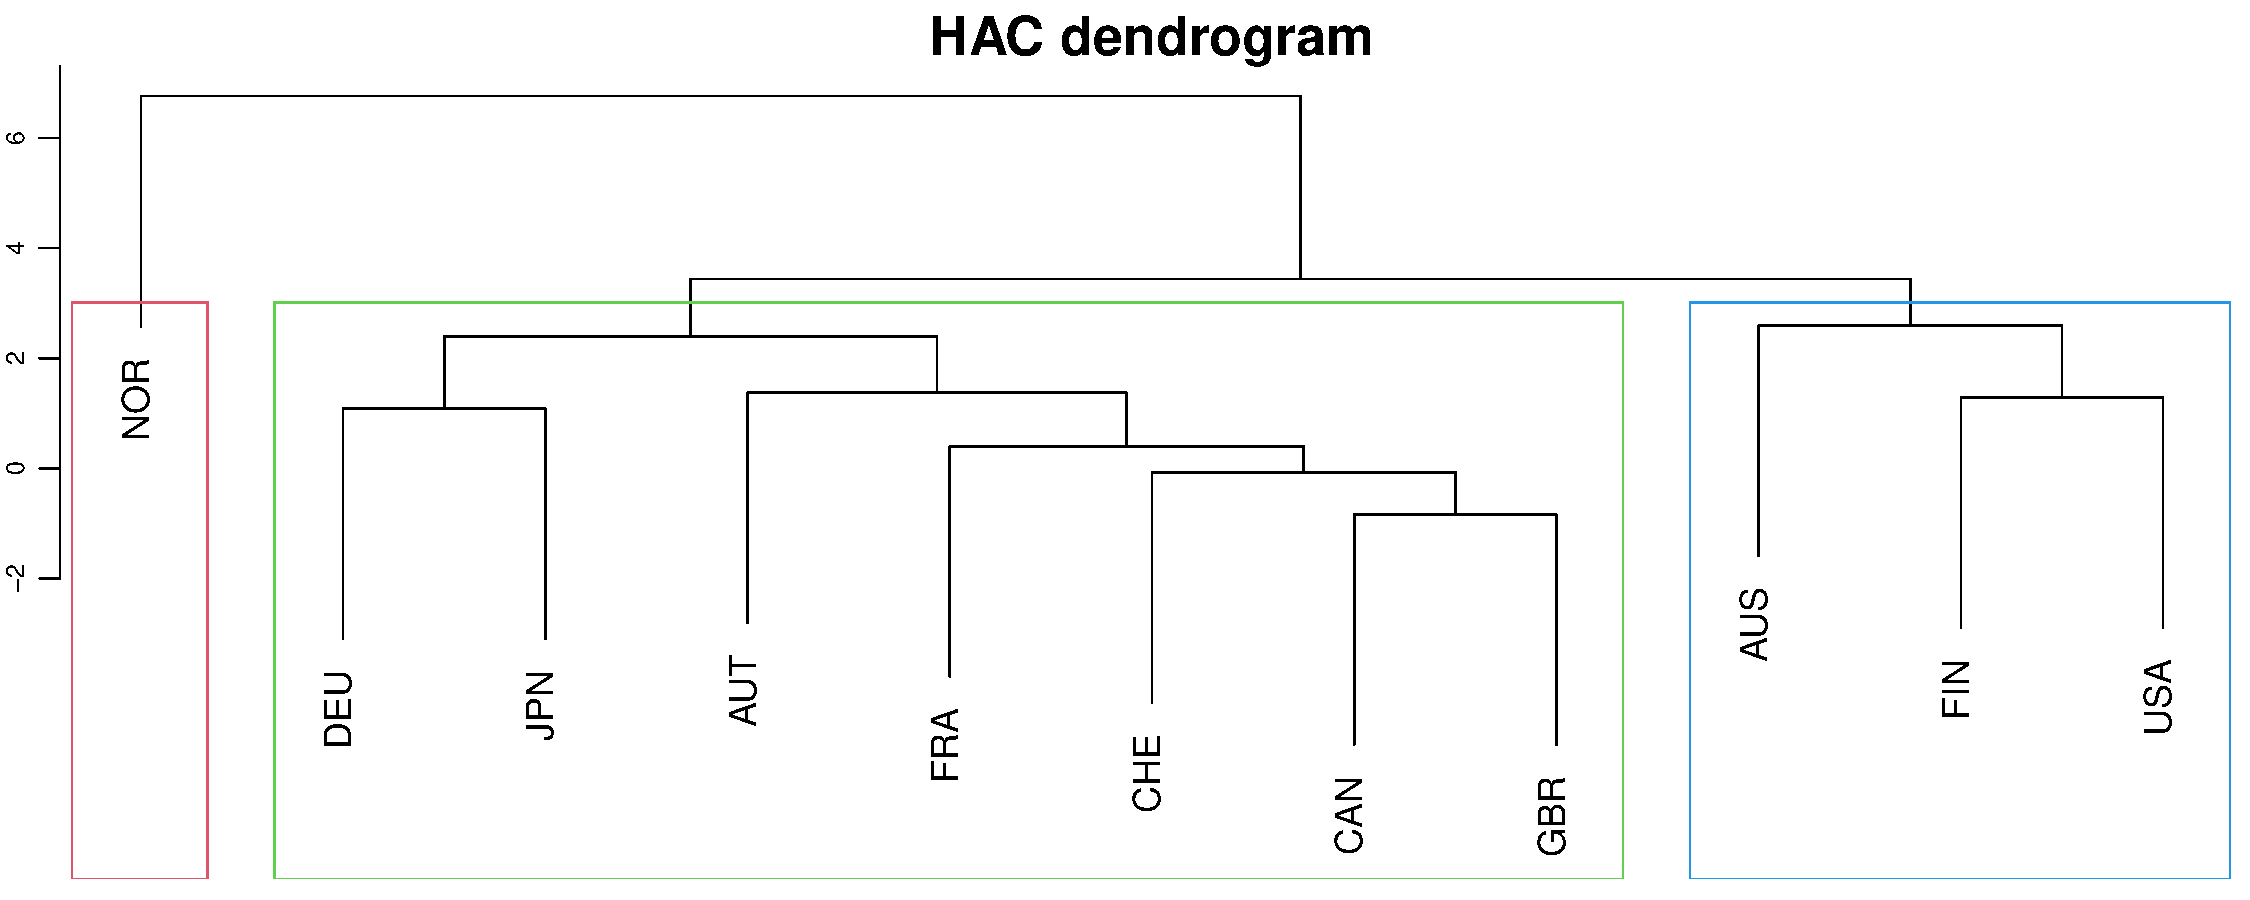
\includegraphics[width=0.95\textwidth]{output/plots/gdp/gdp_dendrogram}
\caption{Dendrogram of a hierarchical agglomerative clustering of GDP time trends for $n = 11$ countries.  Each coloured rectangular corresponds to one of the clusters.}\label{fig:gdp:dend}
\end{center}
\end{figure}

\begin{figure}[t!]
\begin{center}
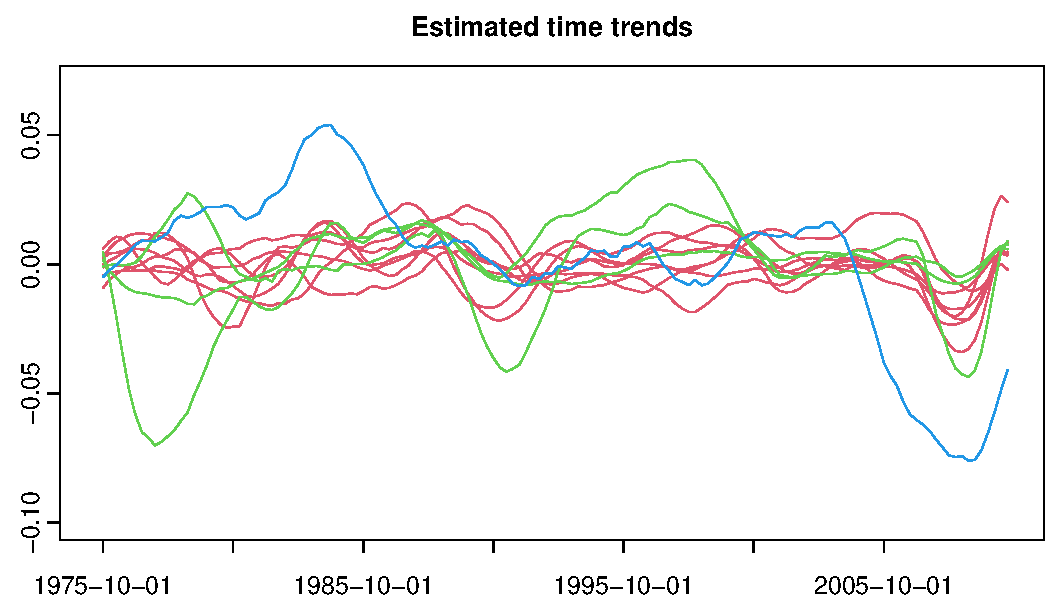
\includegraphics[width=0.95\textwidth]{output/plots/gdp/gdp_all_clusters}
\caption{Local linear kernel estimates of the $n=11$ time trends from the application of Section \ref{subsec:app:gdp} calculated from the augmented time series $\widehat{Y}_{it}$ using the bandwidth $h = 0.05$. Each estimated trend function is coloured according to the cluster that it is assigned to.}\label{fig:gdp:all_clusters}
\end{center}
\end{figure}

Now we briefly comment on the results. Out of $55$ pairwise comparisons, our test detects the differences in the trends $11$ times. In $9$ cases, one of the countries involved in the comparison is Norway; these comparisons are depicted in Figures \ref{fig:Australia:Norway} -- \ref{fig:Japan:Norway}. Note that the differences in the trends seem to be more pronounced towards the end of the considered period: the set of intervals $\mathcal{S}^{[i, j]}(\alpha)$ for those pairs where one of the countries involved in comparison is Norway always covers last $10$ years of the analysed time period (from the first quarter in $2000$ up to the third quarter in $2010$). This coincides with the visual observation mentioned above that in the last $10$ years only Norway exhibited downward movement of the trend in the GDP growth, and this tendency becomes even more pronounced after factoring out the effect of the individual covariates. All of the other countries appear to have a slight increase in the trend function in the same time period. Our test supports this observation.

Figures \ref{fig:USA:France} and \ref{fig:Australia:France} present the results of the pairwise comparison between Australia and France and between the USA and France respectively. In both cases, our test detects the differences between the underlying trends in the GDP growth only in the beginning of the considered time period. In the case of Australia and France, the systematic difference between the trends is clearly visible even in the raw data (panel (a) in Figure~\ref{fig:Australia:France}), whereas in the case of USA and France, the difference is not so obvious. Our test allows us to detect differences in both situations, and we can claim with confidence no less than 95\%, that there are significant differences between the trends for the USA and France (for Australia and France) up to the fourth quarter in 1991 (the fourth quarter in 1987), but there is no evidence of any differences between the trends from 1992 (1988) onwards.

Finally, analysing the results of the clustering algorithm depicted in Figures \ref{fig:gdp:dend} and \ref{fig:gdp:all_clusters}, we also see that our test detected a cluster that consists only of Norway. This supports our observations


\subsection{Analysis of the house prices}\label{subsec:app:hp}

We next analyse the historical dataset on nominal annual house prices from \linebreak\cite{Knoll2017} that contains the data for $14$ advanced economies that covers $143$ years from $1870$ to $2012$.  To ensure minimal manipulation with the data for all time series, we consider observations over the period 1890~--~2012 for 8 countries\footnote{Australia, Belgium, Denmark, France, the Netherlands, Norway, Sweden and the USA.}. Specifically, the data on house prices for all of the countries in our analysis except one (Belgium) contains no missing values, and for Belgium there are only five missing observations\footnote{The missing values in the time series on the house prices for Belgium span five years during the World War I.} which we impute using linear interpolation from the nearest years. Each of the time series for other $6$ countries present in the dataset from \cite{Knoll2017} contains more than $10$ missing values, and hence these countries are excluded from our analysis.



We deflate the nominal house prices with the corresponding consumer price index (CPI) to obtain real house prices ($HP$). Variables that potentially can influence the average house prices are numerous, and there seems to be no general consensus about what the main causes of fluctuations are. Possible determinants include, but are not limited to, demographic factors such as population growth (\citealt{Holly2010}, \citealt{Wang2014}, \citealt{Churchill2021}); fundamental economic factors such as real GDP (\citealt{Huang2013}, \citealt{Churchill2021}), interest rate and inflation (\citealt{Abelson2005}, \citealt{Otto2007}, \citealt{Huang2013}, \citealt{Jorda2015}); urbanisation (\citealt{Chen2011}, \citealt{Wang2017}); government subsidies and regulations (\citealt{Malpezzi1999}); stock markets (\citealt{Gallin2006}); etc. In our analysis, we focus on the following determinants of the average house prices: real GDP ($GDP$), population size ($POP$), long-term interest rate ($I$) and inflation ($INFL$) which is measured as change in CPI. Most other factors (such as government regulations, construction costs, and real wages) vary rather slowly over time and can be captured by time trend, fixed effects and slope heterogeneity.

%\cite{Huang2013} use the GDP growth rate as an explanatory variable for the changes in house price index. \cite{Holly2010} consider a linear parametric model of the logarithm of the house prices, where the control variables include the rate of change in the population and the net cost of borrowing that depends on the long-term interest rate.

%GDP is the most commonly used measure of a country’s economic wellbeing, and has been found to be correlated with house prices (see, e. g., Leung, 2003; Otto, 2007).  Population is an important factor that determines trends relating to the demand and supply of housing, and is therefore often included as a control variable in house price regressions to control for demographic factors as well as potential trends relating to demand and supply (see, e.g., Day, 2018; Engelhardt and Poterba, 1991; Miles, 2012). We also control for interest rate and inflation given that they influence market trends and household ability to finance their homes (Anari and Kolari, 2002; Kuang and Liu, 2015; McQuinn and O’Reilly, 2008; Tang and Tan, 2015; Xu and Tang, 2014).

Data for CPI, real GDP, population size and long-term interest rate are taken from the Jordà-Schularick-Taylor Macrohistory Database,\footnote{See \cite{Jorda2017} for the detailed description of the variable construction.} which is freely available at \linebreak\url{http://www.macrohistory.net/data/} (accessed on 13 January 2022).

\begin{figure}[t!]
\centering

\includegraphics[width=0.8\textwidth]{output/plots/hp/smoothed_hp_data_augmented.pdf}
\vspace{0.2cm}
\caption{Local linear kernel estimates of the $n=8$ augmented time trends from the application of Section \ref{subsec:app:hp}. Each panel shows the estimates for a different bandwidth $h$.}\label{fig:app:hp_augm}
\end{figure}


We thus observe a panel of $n = 8$ time series $\mathcal{T}_i = \{(Y_{it}, \X_{it}): 1 \le t \le T \}$ of length \linebreak$T = 123$ for each country $i \in \{1,\ldots, 8\}$, where $Y_{it} = \ln HP_{it}$ and $\X_{it} = (\ln GDP_{it}, \linebreak \ln POP_{it}, I_{it}, INFL_{it})^\top$. The time series $\mathcal{T}_i$ is assumed to follow the model 
\begin{equation}\label{eq:model:app3}
Y_{it} = \bfbeta^\top_i \X_{it} + m_i \Big( \frac{t}{T} \Big) + \alpha_i + \varepsilon_{it} 
\end{equation}
for $1 \le t \le T$, where $\bfbeta_i = (\beta_{i, 1}, \beta_{i, 2}, \beta_{i, 3}, \beta_{i, 4})^\top$ is a vector of unknown parameters, $m_i$ is a country-specific unknown nonparametric time trend, and $\alpha_i$ is a fixed-effect term. As in Section \ref{subsec:app:gdp}, we rewrite the model \eqref{eq:model:app3} as
\begin{equation}\label{eq:model:app4}
\ln HP_{it} = \beta_{i, 1} \ln GDP_{it} + \beta_{i, 2} \ln POP_{it} + \beta_{i, 3} I_{it} + \beta_{i, 4} INFL_{it} + m_i \Big( \frac{t}{T} \Big) + \alpha_i + \varepsilon_{it}.
\end{equation}

\begin{figure}[b!]
\begin{minipage}[t]{0.49\textwidth}
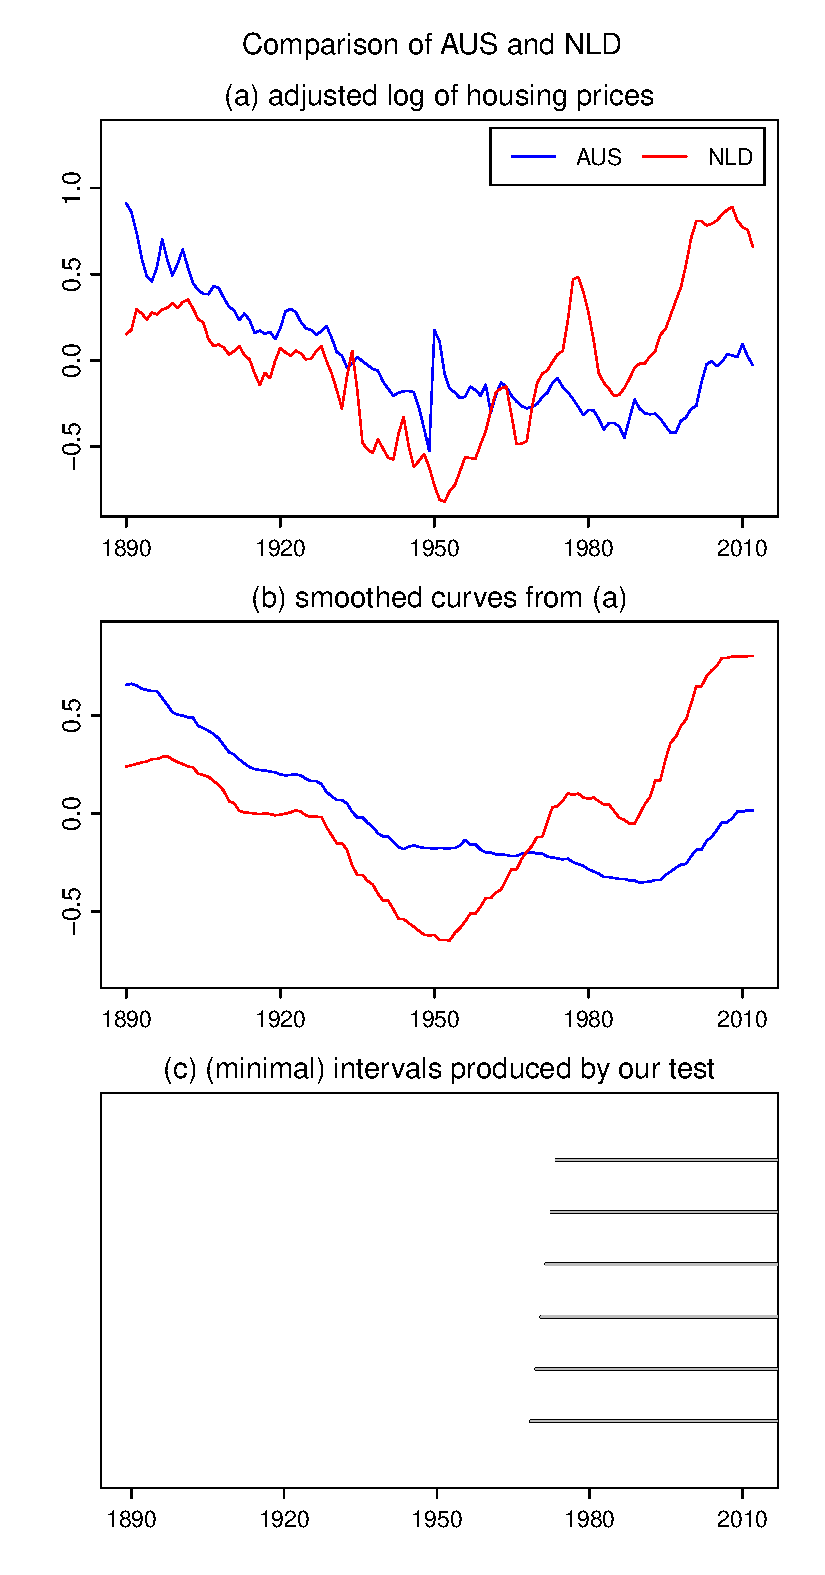
\includegraphics[width=\textwidth]{output/plots/hp/hp_AUS_vs_NLD}
\caption{Test results for the comparison of the housing prices in Australia and the Netherlands.}\label{fig:hp:Australia:Netherlands}
\end{minipage}
\hspace{0.25cm}
\begin{minipage}[t]{0.49\textwidth}
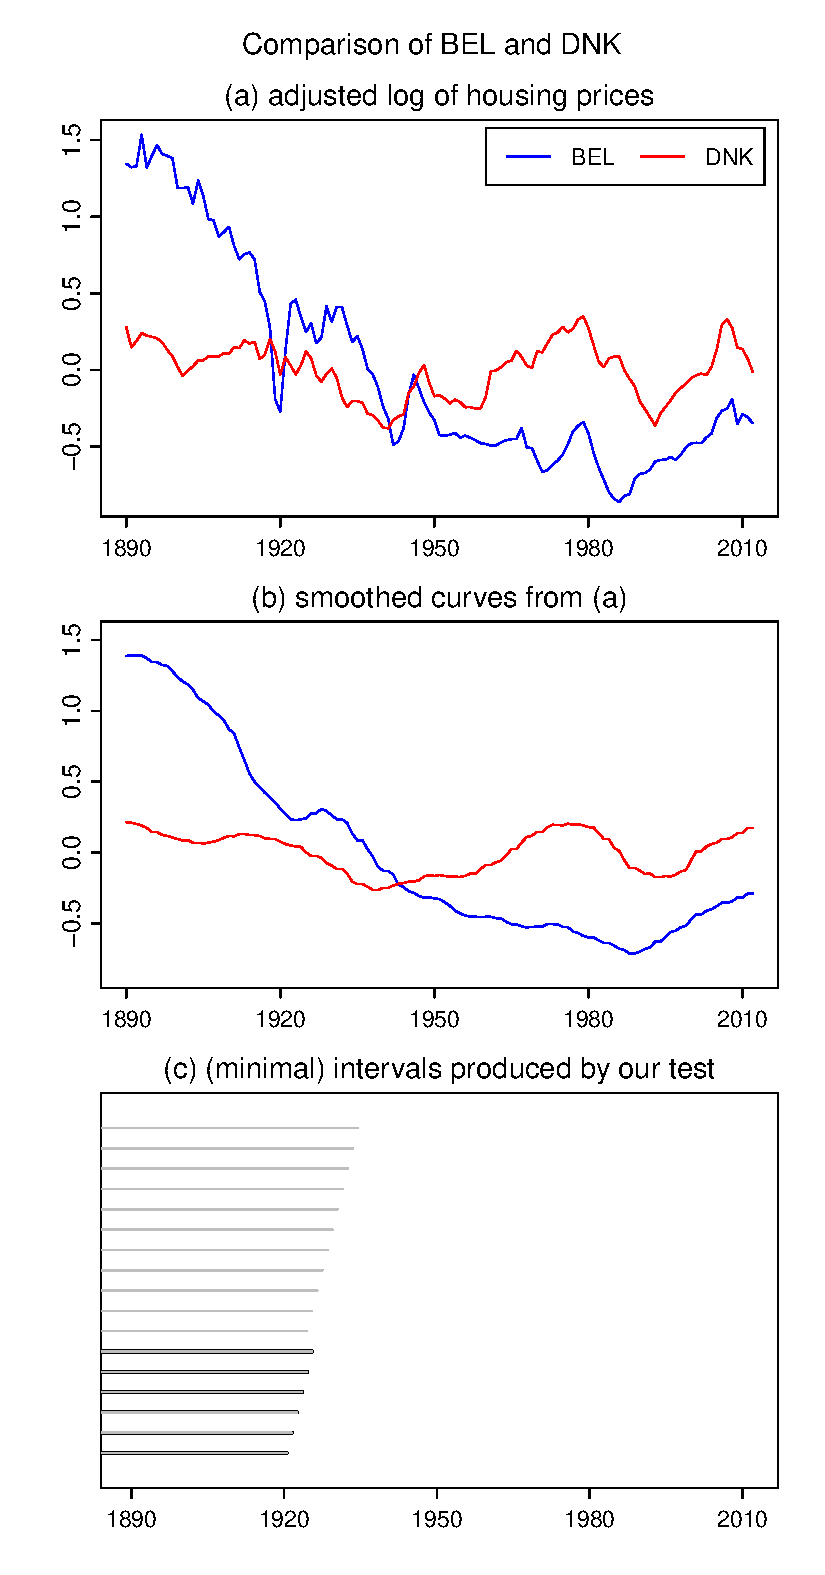
\includegraphics[width=\textwidth]{output/plots/hp/hp_BEL_vs_DNK}
\caption{Test results for the comparison of the housing prices in Belgium and Denmark.}\label{fig:hp:Belgium:Denmark}
\end{minipage}
\caption*{Note: In each figure, panel (a) shows the two augmented time series of the house prices, panel (b) presents smoothed versions of the augmented time series, and panel (c) depicts the set of intervals $\mathcal{S}^{[i, j]}(\alpha)$ in grey and the subset of minimal intervals $\mathcal{S}^{[i, j]}_{min}(\alpha)$ in black.}
\end{figure}

\begin{figure}[t!]
\begin{minipage}[t]{0.49\textwidth}
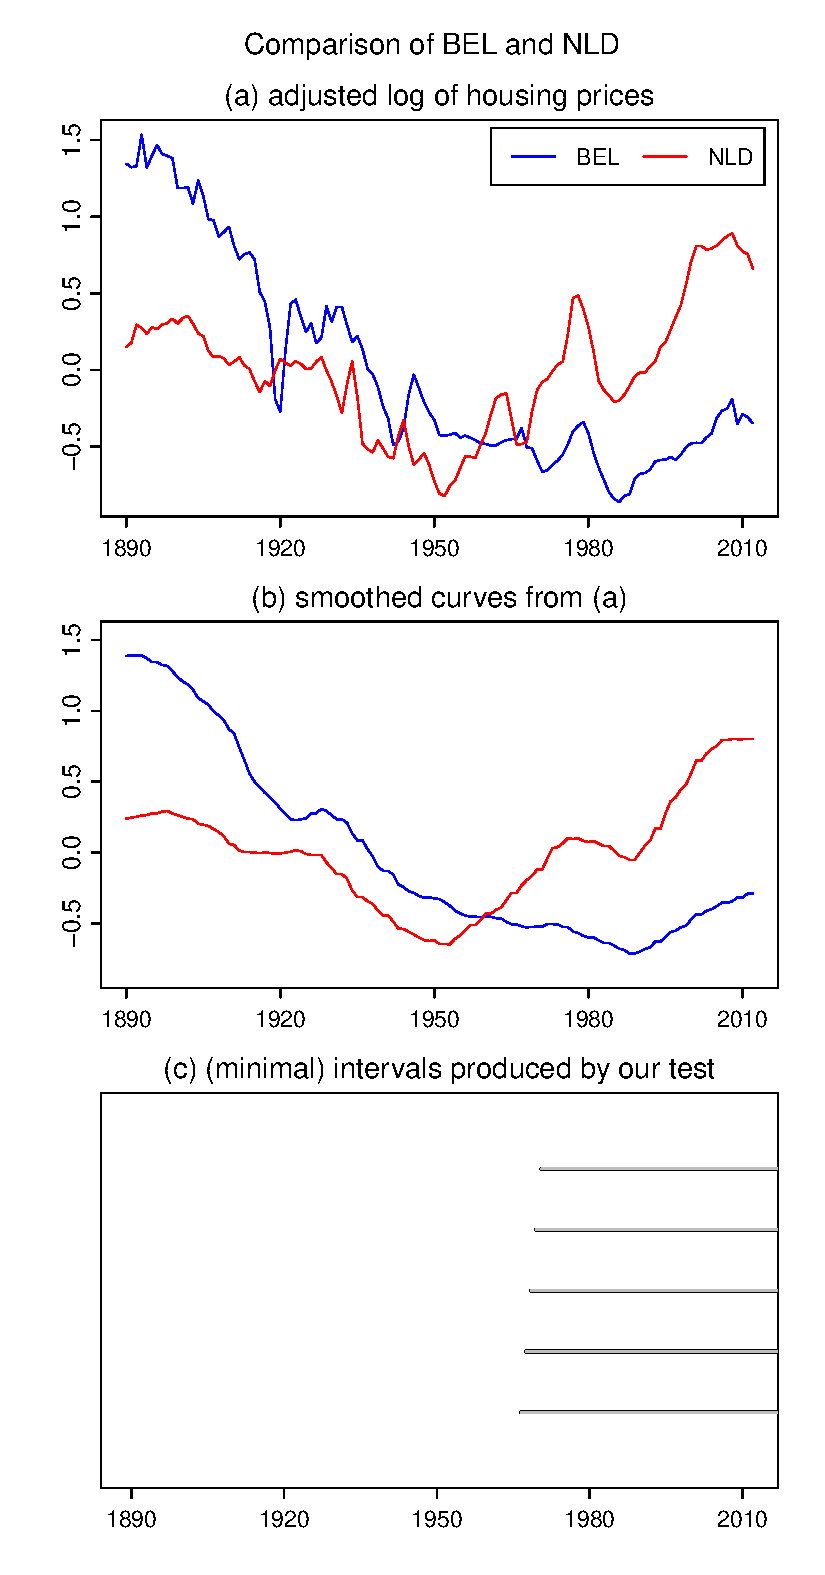
\includegraphics[width=\textwidth]{output/plots/hp/hp_BEL_vs_NLD}
\caption{Test results for the comparison of the housing prices in Belgium and the Netherlands.}\label{fig:hp:Belgium:Netherlands}
\end{minipage}
\hspace{0.25cm}
\begin{minipage}[t]{0.49\textwidth}
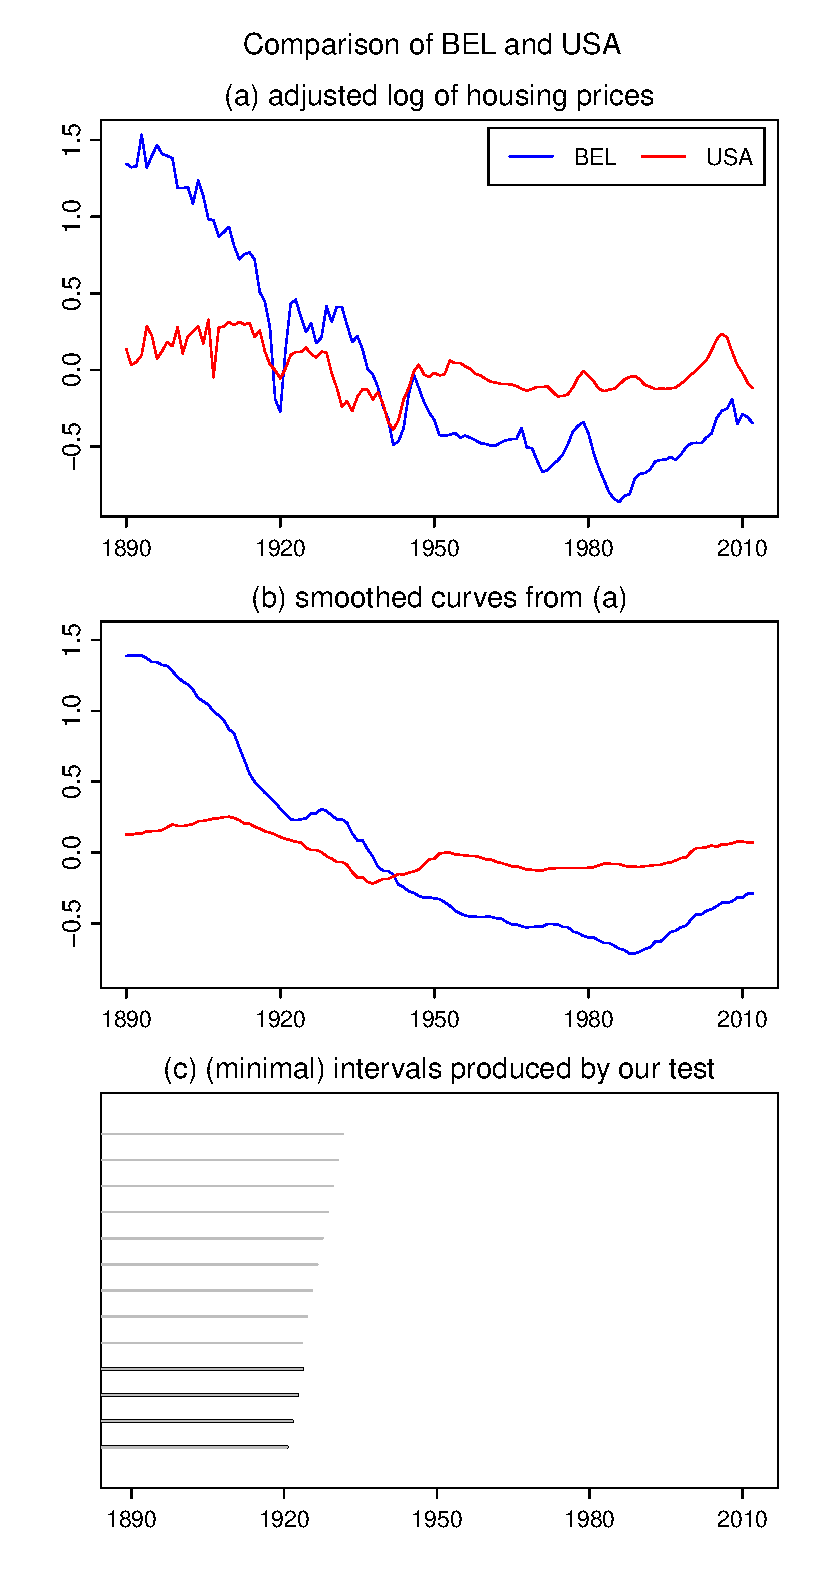
\includegraphics[width=\textwidth]{output/plots/hp/hp_BEL_vs_USA}
\caption{Test results for the comparison of the housing prices in Belgium and the USA.}\label{fig:hp:Belgium:USA}
\end{minipage}
\caption*{Note: In each figure, panel (a) shows the two augmented time series of the house prices, panel (b) presents smoothed versions of the augmented time series, and panel (c) depicts the set of intervals $\mathcal{S}^{[i, j]}(\alpha)$ in grey and the subset of minimal intervals $\mathcal{S}^{[i, j]}_{min}(\alpha)$ in black.}
\end{figure}

The motivation for including nonparametric trend function $m_i$ in the model \ref{eq:model:app4} is supported by the literature. For example, \cite{Ugarte2009} model the temporal trends in average Spanish house prices using splines. \cite{Winter2022} include a long-term trend stochastic component when describing the dynamic behaviour of the time series of real house prices in eight advanced economies. Including nonparametric trend function while modelling the evolution of the house prices is also the main conclusion in \cite{Zhang2016}, where the authors show that the time series for the logarithmic US house prices is trend-stationary, i.e. it can be transformed into a stationary series by subtracting the deterministic trend.

As in Section \ref{subsec:app:gdp}, we assume that for each $i$ the error process $\mathcal{E}_i = \{\varepsilon_{it}: 1 \leq t \leq T\}$ follows an AR($p_i$) model $\varepsilon_{it} = \sum_{j=1}^{p_i} a_{i, j} \varepsilon_{i(t-j)} + \eta_{it}$ with $\eta_{it}$ being the innovations that are i.i.d. across $t$ and have zero mean. As before, we choose $p_i$ as a minimiser of BIC. For $7$ out of $8$ countries the order $p_i$ determined by BIC\footnote{Applying other information criteria such as FPE, AIC and HQ yields exactly the same results in these cases.} is equal to $1$ and, for the sake of simplicity, we assume that $p_i = 1$ for all $i =1, \ldots, 8$.

Our goal is to test whether the time trend $m_i$ is the same in all $8$ countries. In other words, we would like to test the null hypothesis $H_0: m_1 = \ldots = m_n$ with $n = 8$ in the model \eqref{eq:model:app4}. To do so, we implement the multiscale test from Section \ref{sec:test} in the same way as in the previous application example with one minor modification: we let $\mathcal{G}_T = U_T \times H_T$ with 
\begin{align*}
U_T & = \big\{ u \in [0,1]: u = \textstyle{\frac{t}{T}} \text{ for some } t \in \naturals \big\} \\
H_T & = \big\{ h \in \big[ \textstyle{\frac{\log T}{T}}, \textstyle{\frac{1}{4}} \big]:  h = \textstyle{\frac{5t - 3}{T}} \text{ for some } t \in \naturals \big\}. 
\end{align*}
We thus take into account all locations $u$ on an equidistant grid $U_T$ with step length $1/T$ and all bandwidths $h=2/T, 7/T, 12/T,\ldots$ with $\log T /T \le h \le 1/4$. The effective sample sizes are therefore $5, 15, 25, \ldots$ years. As before, the lower bound $\log T / T$ is motivated by Assumption \ref{C-h}.

Apart from this modification, the multiscale test is implemented exactly in the same way as in the simulations of Section \ref{sec:sim} and in the previous application example in Section \ref{subsec:app:gdp}. 

We are now ready to apply the test procedure to the data. Figure \ref{fig:app:hp_augm} depicts local linear estimates of the trend functions $m_i$ for the $n=8$ different countries. Each panel corresponds to a different bandwidth $h$. As can be seen, for all of bandwidths $h$, the fits do not look very similar to each other. On the contrary, there seems to be one country (France) that shows a much more pronounced decrease in the time trend $m_i$ in the first half of the analysed time period than all of the other countries. For the smallest bandwidth value $h = 0.05$, we also see that the behaviour of the trends around year 1950 is not homogeneous. Visual inspection thus suggests that there are strong differences between the time trends $m_i$. Our test confirms this impression. It rejects the null hypothesis at levels $\alpha = 0.05$ and $\alpha = 0.1$. Hence, the test provides evidence for a violation of the null. 

The results of applying our test for level $\alpha= 0.05$ are presented in Figures \ref{fig:hp:Australia:Netherlands} -- \ref{fig:hp:Belgium:USA}. As in Section \ref{subsec:app:gdp}, each figure corresponds to one pairwise comparison $(i, j)$ and is divided into three panels (a) -- (c). The structure of the panels is the same as in Figures \ref{fig:Australia:Norway} -- \ref{fig:Australia:France}: Panel (a) shows the augmented time series $\{\widehat{Y}_{it}: 1 \le t \le T\}$ and $\{\widehat{Y}_{jt}: 1 \le t \le T\}$ for the two countries $i$ and $j$. Panel (b) presents smoothed versions of the time series from (a) with the bandwidth window covering $15$ years. Finally, panel (c) presents the results produced by our test for a significance level $\alpha = 0.05$. As before, the set of rejected intervals $\mathcal{S}^{[i, j]}(\alpha)$ and the set of minimal intervals $\mathcal{S}^{[i, j]}_{min}(\alpha) \subseteq \mathcal{S}^{[i, j]}(\alpha)$ are depicted in grey and in black respectively. 

Our findings coincide with the observations in \cite{Knoll2017}, where the authors find considerable cross-country heterogeneity in the trends in house prices. Moreover, according to \eqref{corollary1}, we can make the following simultaneous confidence statement about the intervals plotted in panels (c) of Figures \ref{fig:hp:Australia:Netherlands} -- \ref{fig:hp:Belgium:USA}: we can claim, with confidence of about $95\%$, that there is a difference between the functions $m_i$ and $m_j$ on each of these intervals. 

\section{Conclusion}\label{sec:conclusion}

In this paper, we develop a new multiscale testing procedure for multiple time series for testing hypotheses about nonparametric time trends in the presence of covariates. This procedure addresses two important statistical problems about comparison of the time trends. First and foremost, with the help of the proposed method, we are able to test if all the time trends in the observed time series are the same or not. We prove the main theoretical results of the paper that the test has (asymptotically) the correct size and has an (asymptotic) power of one against a specific class of local alternatives. Second, our multiscale procedure allows us to tell which of the time trends are different and where the differences are located. For the purpose of pinpointing the differences, we consider many local null hypotheses at the same time, each corresponding to only two time trends and a specific time interval. Our method allows us to test all of these hypotheses simultaneously controlling the family-wise error rate, i.e. the probability of wrongly rejecting at least one true null hypothesis (making at least one type I error), at a desired level $\alpha$. This result allows us to make simultaneous confidence statements as follows: 

\begin{center}
\begin{minipage}[c][1.75cm][c]{14cm}
\textit{We can state with (asymptotic) probability at least $1-\alpha$ that for every pair of time series and every interval where our test rejects the local null, the trends of these time series differ at least somewhere on this particular interval.}
\end{minipage}
\end{center}

For the proof of the theoretical results, the main tools that are used are strong approximation theory developed in \cite{BerkesLiuWu2014} and the anti-concentration bounds for Gaussian random vectors verified in \cite{Chernozhukov2015}. The proof strategy that we employ in our paper has already been used in \cite{KhismatullinaVogt2020}, however, in that paper the authors proposed a multiscale method for testing qualitative hypotheses only about one time series. Our method can be regarded as a generalised version of the test developed in \cite{KhismatullinaVogt2020} where we not only consider comparison between various time series, but also add the covariates to the model and propose an estimation procedure for the unknown parameters.

Regarding future research, this project suggests some interesting issues and topics for consideration. \textcolor{red}{First, as was already mentioned, it should be possible to extend our theoretical results to the case where the number of time series slowly grows with the sample size. Second, the theory in this paper is developed under the assumption that the first differences of the covariates and of error terms are uncorrelated. This restriction limits possible applications of our method. Further insight can be gained by broadening the current work in these and possibly other directions.}

\newpage
\bibliographystyle{ims}
{\small
\setlength{\bibsep}{0.55em}
\bibliography{bibliography}}

\allowdisplaybreaks[3]
\section{Appendix}\label{sec-appendix}

\subsection{Proof of Theorem \ref{theo-regs}}\label{subsec-appendix-estimators}

We define the first-differenced regressors as follows.
\[ \Delta \mathbf{X}_{it} =\mathbf{H}_i(\mathcal{U}_{it}) - \mathbf{H}_i(\mathcal{U}_{it-1}) := \Delta \mathbf{H}_i(\mathcal{U}_{it}). \]
Similarly, 
\[\Delta \varepsilon_{it} = \varepsilon_{it} - \varepsilon_{it-1} = G_i(\mathcal{J}_{it}) - G_i(\mathcal{J}_{it-1}) = \Delta G_i(\mathcal{J}_{it}).
\]
 
With these assumptions we can prove the following propositions.
\begin{prop}\label{prop-reg-1}
Under Assumptions \ref{C-reg1} and \ref{C-reg3}, $|| \Delta \mathbf{H}_i(\mathcal{U}_{it})||_4 < \infty$.
\end{prop}

\begin{proof}[\textnormal{\textbf{Proof of Proposition \ref{prop-reg-1}}}]
By Assumption \ref{C-reg3},
\[
 || \Delta \mathbf{H}_i(\mathcal{U}_{it})||_4 \leq  ||\mathbf{H}_i(\mathcal{U}_{it})||_4 +  || \mathbf{H}_i(\mathcal{U}_{it-1})||_4 < \infty.
\]
\end{proof} 

\begin{prop}\label{prop-reg-2}
Under Assumption \ref{C-reg4}, $\Delta \mathbf{X}_{it}$ (elementwise) and $\Delta \varepsilon_{it}$ are uncorrelated for each $t\in \{1, \ldots, T\}$.
\end{prop}

\begin{proof}[\textnormal{\textbf{Proof of Proposition \ref{prop-reg-2}}}]
By Assumption \ref{C-reg4},
\begin{align*}
\ex [\Delta \mathbf{X}_{it}\Delta \varepsilon_{it}] &= \ex \big[(\mathbf{X}_{it} - \mathbf{X}_{it-1}) (\varepsilon_{it} - \varepsilon_{it-1})\big] =\\
=&\ex[\mathbf{X}_{it}  \varepsilon_{it}] - \ex[\mathbf{X}_{it-1}  \varepsilon_{it}]- \ex[\mathbf{X}_{it}  \varepsilon_{it-1}] + \ex[\mathbf{X}_{it-1}  \varepsilon_{it-1}] =\\
=& \ex[\mathbf{X}_{it}]\ex[  \varepsilon_{it}] - \ex[\mathbf{X}_{it-1}]\ex[  \varepsilon_{it}]- \ex[\mathbf{X}_{it}]\ex[  \varepsilon_{it-1}] + \ex[\mathbf{X}_{it-1}]\ex[  \varepsilon_{it-1}] =\\
=& \big( \ex[\mathbf{X}_{it}] - \ex[\mathbf{X}_{it-1}]\big)\big(\ex[  \varepsilon_{it}]  - \ex[\varepsilon_{it-1}]\big) = \ex [\Delta \mathbf{X}_{it}]\ex[\Delta \varepsilon_{it}]
\end{align*}
\end{proof} 


\begin{prop}\label{prop-reg-3}
Define 
\[ \Delta \mathbf{U}_i(\mathcal{I}_{i, t}) := \Delta \mathbf{H}_i(\mathcal{U}_{it}) \Delta G_i(\mathcal{J}_{it}).
\]
Under Assumptions \ref{C-err2} - \ref{C-err3}, \ref{C-reg5} - \ref{C-reg6}, we have that $\sum_{s=0}^\infty \delta_2(\Delta \mathbf{U}_i, s) < \infty$.
\end{prop}

\begin{proof}[\textnormal{\textbf{Proof of Proposition \ref{prop-reg-3}}}]
Note the following
\begin{align*}
 &\delta_2(\Delta \mathbf{U}_i, t) = || \Delta\mathbf{U}_i(\mathcal{I}_{i, t}) - \Delta \mathbf{U}_i(\mathcal{I}_{i,t}^\prime) ||_2 =\\
 &= || \Delta \mathbf{H}_i(\mathcal{U}_{it}) \Delta G_i(\mathcal{J}_{it}) -  \Delta \mathbf{H}_i(\mathcal{U}_{it}^\prime) \Delta G_i(\mathcal{J}_{it}^\prime) ||_2 =\\
 & = ||\big(\mathbf{H}_i(\mathcal{U}_{it}) - \mathbf{H}_i(\mathcal{U}_{it-1})\big)\big(G_i(\mathcal{J}_{it}) - G_i(\mathcal{J}_{it-1})\big) - \big(\mathbf{H}_i(\mathcal{U}_{it}^\prime) - \mathbf{H}_i(\mathcal{U}_{it-1}^\prime)\big)\big(G_i(\mathcal{J}_{it}^\prime) - G_i(\mathcal{J}_{it-1}^\prime)\big)||_2 =\\
 &= ||\mathbf{H}_i(\mathcal{U}_{it})G_i(\mathcal{J}_{it}) - \mathbf{H}_i(\mathcal{U}_{it-1})G_i(\mathcal{J}_{it}) - \mathbf{H}_i(\mathcal{U}_{it})G_i(\mathcal{J}_{it-1})  + \mathbf{H}_i(\mathcal{U}_{it-1})G_i(\mathcal{J}_{it-1}) - \\
 &\quad - \mathbf{H}_i(\mathcal{U}_{it}^\prime)G_i(\mathcal{J}_{it}^\prime) + \mathbf{H}_i(\mathcal{U}_{it-1}^\prime)G_i(\mathcal{J}_{it}^\prime) + \mathbf{H}_i(\mathcal{U}_{it}^\prime)G_i(\mathcal{J}_{it-1}^\prime)  - \mathbf{H}_i(\mathcal{U}_{it-1}^\prime)G_i(\mathcal{J}_{it-1}^\prime) ||_2\leq \\
 &\leq ||\mathbf{H}_i(\mathcal{U}_{it})G_i(\mathcal{J}_{it}) - \mathbf{H}_i(\mathcal{U}_{it}^\prime)G_i(\mathcal{J}_{it}^\prime) ||_2 + ||\mathbf{H}_i(\mathcal{U}_{it-1})G_i(\mathcal{J}_{it-1}) -  \mathbf{H}_i(\mathcal{U}_{it-1}^\prime)G_i(\mathcal{J}_{it-1}^\prime)||_2 + \\
 &\quad + ||\mathbf{H}_i(\mathcal{U}_{it-1})G_i(\mathcal{J}_{it}) -\mathbf{H}_i(\mathcal{U}_{it-1}^\prime)G_i(\mathcal{J}_{it}^\prime)    ||_2
 + ||\mathbf{H}_i(\mathcal{U}_{it})G_i(\mathcal{J}_{it-1}) -  \mathbf{H}_i(\mathcal{U}_{it}^\prime)G_i(\mathcal{J}_{it-1}^\prime) ||_2 = \\
 & = \delta_2(\mathbf{U}_i, t) + \delta_2(\mathbf{U}_i, t-1)  +\\
 &\quad + ||\mathbf{H}_i(\mathcal{U}_{it-1})G_i(\mathcal{J}_{it}) - \mathbf{H}_i(\mathcal{U}_{it-1}^\prime)G_i(\mathcal{J}_{it}) + \mathbf{H}_i(\mathcal{U}_{it-1}^\prime)G_i(\mathcal{J}_{it}) - \mathbf{H}_i(\mathcal{U}_{it-1}^\prime)G_i(\mathcal{J}_{it}^\prime)    ||_2+\\
 &\quad + ||\mathbf{H}_i(\mathcal{U}_{it})G_i(\mathcal{J}_{it-1}) -\mathbf{H}_i(\mathcal{U}_{it}^\prime)G_i(\mathcal{J}_{it-1})+ \mathbf{H}_i(\mathcal{U}_{it}^\prime)G_i(\mathcal{J}_{it-1})-  \mathbf{H}_i(\mathcal{U}_{it}^\prime)G_i(\mathcal{J}_{it-1}^\prime) ||_2 \leq\\
  &\leq \delta_2(\mathbf{U}_i, t) + \delta_2(\mathbf{U}_i, t-1)  + \\
  &\quad +||\big(\mathbf{H}_i(\mathcal{U}_{it-1}) - \mathbf{H}_i(\mathcal{U}_{it-1}^\prime)\big) G_i(\mathcal{J}_{it})||_2 +  ||\mathbf{H}_i(\mathcal{U}_{it-1}^\prime)\big(G_i(\mathcal{J}_{it}) - G_i(\mathcal{J}_{it}^\prime)\big)    ||_2+\\
 &\quad + ||\big(\mathbf{H}_i(\mathcal{U}_{it}) -\mathbf{H}_i(\mathcal{U}_{it}^\prime)\big)G_i(\mathcal{J}_{it-1})||_2 + ||\mathbf{H}_i(\mathcal{U}_{it}^\prime)\big(G_i(\mathcal{J}_{it-1}) -G_i(\mathcal{J}_{it-1}^\prime)\big) ||_2 \leq \\
 &\leq \delta_2(\mathbf{U}_i, t) + \delta_2(\mathbf{U}_i, t-1)  + \big(\delta_2(\mathbf{H}_i, t-1) +  \delta_2(\mathbf{H}_i, t)\big) ||G_i ||_2+ \big( \delta_2(G_i, t-1) +  \delta_2(G_i, t)\big)||\mathbf{H}_i ||_2  
\end{align*}

Here $\mathcal{U}_{it}^\prime  = (\ldots, u_{i(-1)}, u^\prime_{i0}, u_{i1}, \ldots, u_{it-1}, u_{it})$, $\mathcal{U}_{it-1}^\prime  = (\ldots, u_{i(-1)}, u^\prime_{i0}, u_{i1}, \ldots, u_{it-1})$, $\mathcal{J}_{it}^\prime  = (\ldots, \eta_{i(-1)}, \eta^\prime_{i0}, \eta_{i1}, \ldots, \eta_{it-1}, \eta_{it})$, $\mathcal{J}_{it-1}^\prime  = (\ldots, \eta_{i(-1)}, \eta^\prime_{i0}, \eta_{i1}, \ldots, \eta_{it-1})$ are coupled processes with $u_{i0}^\prime$ being an i.i.d. copy of $u_{i0}$ and $\eta_{i0}^\prime$ being an i.i.d. copy of $\eta_{i0}$.

This leads us to 
\begin{align*}
 &\sum_{s=0}^\infty \delta_2(\Delta \mathbf{U}_i, s) \leq \sum_{s=0}^\infty \delta_2(\mathbf{U}_i, s) + \sum_{s=1}^\infty\delta_2(\mathbf{U}_i, s-1)  +\\
 &\quad + \sum_{s=1}^\infty\big(\delta_2(\mathbf{H}_i, s-1) +  \delta_2(\mathbf{H}_i, s)\big) ||G_i ||_2 + \sum_{s=1}^\infty\big( \delta_2(G_i, s-1) +  \delta_2(G_i, s)\big)||\mathbf{H}_i ||_2 <\infty 
\end{align*}


\end{proof}


\begin{prop}\label{prop-reg-4}
Under Assumptions \ref{C-err1} - \ref{C-reg6},
\[ \Big| \frac{1}{\sqrt{T}}\sum_{t=1}^T \Delta \mathbf{X}_{it}\Delta \varepsilon_{it} \Big| = O_P(1).
\]
\end{prop}

\begin{proof}[\textnormal{\textbf{Proof of Proposition \ref{prop-reg-4}}}]
We need the following notation:
\begin{alignat*}{2}
&\mathcal{P}_{i,t}(\cdot) &&:= \ex[\cdot|\mathcal{I}_{i, t}] -\ex[\cdot|\mathcal{I}_{i, t-1}], \\
&\kappa_{i} && := \frac{1}{T}\sum_{t=1}^T  \Delta \mathbf{X}_{it}\Delta \varepsilon_{it}, \\
&\kappa_{i, s}^{\mathcal{P}} && := \frac{1}{T}\sum_{t=1}^T \mathcal{P}_{i, t-s}\big( \Delta \mathbf{X}_{it}\Delta \varepsilon_{it}\big).
\end{alignat*}
Then,
\begin{align*}
||\kappa_{i, s}^{\mathcal{P}}||^2 &= \Big|\Big| \frac{1}{T}\sum_{t=1}^T \mathcal{P}_{i, t-s}\big( \Delta \mathbf{X}_{it}\Delta \varepsilon_{it}\big) \Big|\Big|^2 \leq\\
&\leq \frac{1}{T^2} \sum_{t=1}^T \Big|\Big| \ex (\Delta \mathbf{X}_{it}\Delta \varepsilon_{it}|\mathcal{I}_{i, t-s}) -\ex (\Delta \mathbf{X}_{it}\Delta \varepsilon_{it}|\mathcal{I}_{i, t-s-1}) \Big|\Big|^2 =\\
&= \frac{1}{T^2} \sum_{t=1}^T \Big|\Big| \ex (\Delta \mathbf{X}_{it}\Delta \varepsilon_{it}|\mathcal{I}_{i, t-s}) -\ex (\Delta \mathbf{X}_{it, s}^\prime\Delta \varepsilon_{it, s}^\prime|\mathcal{I}_{i, t-s}) \Big|\Big|^2,
\end{align*}
where $\Delta \mathbf{X}_{it, s}^\prime\Delta \varepsilon_{it, s}^\prime$ denotes $\Delta \mathbf{X}_{it}\Delta \varepsilon_{it}$ with $\{\zeta_{i, t-s}\}$ replaced by its i.i.d. copy $\{\zeta_{i, t-s}^\prime\}$. In this case $\ex (\Delta \mathbf{X}_{it, s}^\prime\Delta \varepsilon_{it, s}^\prime|\mathcal{I}_{i, t-s -1}) = \ex (\Delta \mathbf{X}_{it, s}^\prime\Delta \varepsilon_{it, s}^\prime|\mathcal{I}_{i, t-s})$. Furthermore, by linearity of the expectation and Jensen's inequality, we have 
\begin{align*}
||\kappa_{i, s}^{\mathcal{P}}||^2 &\leq \frac{1}{T^2} \sum_{t=1}^T \Big|\Big| \ex (\Delta \mathbf{X}_{it}\Delta \varepsilon_{it}|\mathcal{I}_{i, t-s}) -\ex (\Delta \mathbf{X}_{it, s}^\prime\Delta \varepsilon_{it, s}^\prime|\mathcal{I}_{i, t-s}) \Big|\Big|^2 \leq \\
&\leq \frac{1}{T^2} \sum_{t=1}^T \Big|\Big| \Delta \mathbf{X}_{it}\Delta \varepsilon_{it} -\Delta \mathbf{X}_{it, s}^\prime\Delta \varepsilon_{it, s}^\prime\Big|\Big|^2 =\\
& = \frac{1}{T^2} \sum_{t=1}^T \Big|\Big| \Delta \mathbf{H}_i(\mathcal{U}_{it})  \Delta G_i(\mathcal{J}_{it}) - \Delta \mathbf{H}_i(\mathcal{U}_{it, s}^\prime)  \Delta G_i(\mathcal{J}_{it, s}^\prime)\Big|\Big|^2 =\\
& = \frac{1}{T^2} \sum_{t=1}^T \Big|\Big| \Delta \mathbf{U}_i(\mathcal{I}_{i,t})  - \Delta \mathbf{U}_i(\mathcal{I}_{i,t, s}^\prime) \Big|\Big|^2 \leq \frac{1}{T^2} \sum_{t=1}^T \delta_2^2(\Delta \mathbf{U}_i, s) = \frac{1}{T}\delta_2^2(\Delta \mathbf{U}_i, s)
\end{align*}
with $\mathcal{U}_{it, s}^\prime = (\ldots, u_{it-s-1}, u^\prime_{it-s}, u_{it-s+1}, \ldots, u_{it})$, $\mathcal{J}_{it, s}^\prime = (\ldots, \eta_{it-s-1}, \eta^\prime_{it-s}, \eta_{it-s+1}, \ldots, \eta_{it})$, $\zeta^\prime_{it} = (u_{it}^\prime, \eta_{it}^\prime)^\top$ and $\mathcal{I}_{i,t,s}^\prime =(\ldots, \zeta_{it-s-1}, \zeta^\prime_{it-s}, \zeta_{it-s+1}, \ldots, \zeta_{it})$.

Moreover,
\begin{align*}
\kappa_i - \ex \kappa_i &= \frac{1}{T}\sum_{t=1}^T \Delta \mathbf{X}_{it}\Delta \varepsilon_{it} - \ex \kappa_i = \frac{1}{T}\sum_{t=1}^T \ex ( \Delta \mathbf{X}_{it}\Delta \varepsilon_{it}|\mathcal{I}_{i,t}) - \ex \kappa_i =\\
&= \frac{1}{T}\sum_{t=1}^T \big( \ex ( \Delta \mathbf{X}_{it}\Delta \varepsilon_{it}|\mathcal{I}_{i,t} ) - \ex ( \mathbf{X}_{it}\Delta \varepsilon_{it}) \big) = \\
&= \frac{1}{T}\sum_{t=1}^T \sum_{s=0}^\infty \big( \ex ( \Delta \mathbf{X}_{it}\Delta \varepsilon_{it}|\mathcal{I}_{i,t-s} ) - \ex ( \Delta \mathbf{X}_{it}\Delta \varepsilon_{it}|\mathcal{I}_{i,t-s-1} )  \big) =\\
&= \frac{1}{T}\sum_{t=1}^T \sum_{s=0}^\infty \mathcal{P}_{i, t-s} (\Delta \mathbf{X}_{it}\Delta \varepsilon_{it}) = \sum_{s=0}^\infty \kappa_{i, s}^{\mathcal{P}}.
\end{align*}
Thus, by Proposition \ref{prop-reg-3},
\[ || \kappa_i - \ex \kappa_i || \leq \sum_{s=0}^\infty ||\kappa_{i, s}^{\mathcal{P}} || \leq \frac{1}{\sqrt{T}}\sum_{s=0}^\infty \delta_2(\Delta \mathbf{U}_i, s) = O\Big(\frac{1}{\sqrt{T}}\Big)
\]
Since $\ex \kappa_i = 0$ by Proposition \ref{prop-reg-2}, we conclude that
\[  \Big|\Big| \frac{1}{T}\sum_{t=1}^T  \Delta \mathbf{X}_{it}\Delta \varepsilon_{it} \Big|\Big| = O\Big(\frac{1}{\sqrt{T}}\Big).
\]
Therefore, the proposition follows.
\end{proof}



\begin{proof}[\textnormal{\textbf{Proof of Theorem \ref{theo-regs}}}]
Recall the differencing estimator $\widehat{\bm{\beta}}_i$:
\begin{align*}
\widehat{\bm{\beta}}_i &= \Big( \sum_{t=1}^T \Delta \mathbf{X}_{it} \Delta \mathbf{X}_{it}^\top \Big)^{-1} \sum_{t=1}^T \Delta \mathbf{X}_{it} \Delta Y_{it} =\\
& =  \Big( \sum_{t=1}^T \Delta \mathbf{X}_{it} \Delta \mathbf{X}_{it}^\top \Big)^{-1} \sum_{t=1}^T \Delta \mathbf{X}_{it} \bigg(\Delta \mathbf{X}_{it}^\top \bm{\beta}_i + \Delta \varepsilon_{it} + O\Big(\frac{1}{T}\Big) \bigg) =\\
&= \bm{\beta}_i +  \Big( \sum_{t=1}^T \Delta \mathbf{X}_{it} \Delta \mathbf{X}_{it}^\top \Big)^{-1} \sum_{t=1}^T \Delta \mathbf{X}_{it} \Delta \varepsilon_{it}
+  O\Big(\frac{1}{T}\Big) \Big( \sum_{t=1}^T \Delta \mathbf{X}_{it} \Delta \mathbf{X}_{it}^\top \Big)^{-1} \sum_{t=1}^T \Delta \mathbf{X}_{it}. 
\end{align*}
This leads to
\begin{align*}
\sqrt{T}( \widehat{\bm{\beta}}_i - \bm{\beta}_i) &=  \Big(\frac{1}{T} \sum_{t=1}^T \Delta \mathbf{X}_{it} \Delta \mathbf{X}_{it}^\top \Big)^{-1}\frac{1}{\sqrt{T}} \sum_{t=1}^T \Delta \mathbf{X}_{it} \Delta \varepsilon_{it} +\\
&+  O\Big(\frac{1}{\sqrt{T}}\Big) \Big( \frac{1}{T}\sum_{t=1}^T \Delta \mathbf{X}_{it} \Delta \mathbf{X}_{it}^\top \Big)^{-1} \frac{1}{T}\sum_{t=1}^T \Delta \mathbf{X}_{it}.
\end{align*}

Since 
\[\ex \Big[ \frac{1}{T}\sum_{t=1}^T \Delta H_{ij}(\mathcal{U}_{it})\Big] = 0\]
and 
\[\var \Big[ \frac{1}{T}\sum_{t=1}^T \Delta H_{ij}(\mathcal{U}_{it})\Big] \leq \frac{4}{T^2} \ex\big[H_{ij}^2(\mathcal{U}_{it})\big],\]
by Chebyshev's inequality we have that $\Big|\frac{1}{T}\sum_{t=1}^T \Delta H_{ij}(\mathcal{U}_{it})\Big| = O_P(1)$ for each $j\in\{1, \ldots, d\} $. And this in turn implies that
\begin{align}\label{proof-1}
\Big|\frac{1}{T}\sum_{t=1}^T \Delta \mathbf{H}_i (\mathcal{U}_{it}) \Big| = \Big| \frac{1}{T}\sum_{t=1}^T \Delta \mathbf{X}_{it}\Big| = O_P(1).
\end{align}


Similarly, by Proposition \ref{prop-reg-1} and Chebyshev's inequality, we have that for each $j, k\in\{1, \ldots, d\}$
\[  \Big|\frac{1}{T}\sum_{t=1}^T \Delta H_{ij}(\mathcal{U}_{it}) \Delta H_{ik}(\mathcal{U}_{it})\Big| = O_P(1),
\]
which leads to 
\begin{align}\label{proof-2}
\Big|\Big| \frac{1}{T}\sum_{t=1}^T \Delta \mathbf{H}_i (\mathcal{U}_{it})\Delta \mathbf{H}_i (\mathcal{U}_{it})^\top \Big|\Big| =\Big|\Big|\frac{1}{T}\sum_{t=1}^T\Delta \mathbf{X}_{it} \Delta \mathbf{X}_{it}^\top\Big|\Big| = O_P(1),
\end{align}
where $||A||$ with $A$ being a matrix is any matrix norm.

By Assumption \ref{C-reg2}, we know that $\ex [\Delta \mathbf{X}_{it} \Delta \mathbf{X}_{it}^\top] = \ex [\Delta \mathbf{X}_{i0} \Delta \mathbf{X}_{i0}^\top]$ is invertible, thus, 
\[\Bigg| \Bigg| \Big(\frac{1}{T}\sum_{t=1}^T\Delta \mathbf{X}_{it} \Delta \mathbf{X}_{it}^\top\Big)^{-1}\Bigg|\Bigg| = O_P(1).\]
By applying Proposition \ref{prop-reg-4}, \eqref{proof-1} and \eqref{proof-2}, the statement of the theorem follows.
\end{proof}

\subsection{Proof of Theorem \ref{theo-stat-equality}}\label{subsec-appendix-stat-equaility}


In this section, we prove the theoretical results from Section \ref{sec-method}. We use the following notation: The symbol $C$ denotes a universal real constant which may take a different value on each occurrence. For $a,b \in \reals$, we write $a_+ = \max \{0,a\}$ and $a \vee b = \max\{a,b\}$. For any set $A$, the symbol $|A|$ denotes the cardinality of $A$. The notation $X \stackrel{\mathcal{D}}{=} Y$ means that the two random variables $X$ and $Y$ have the same distribution. Finally, $f_0(\cdot)$ and $F_0(\cdot)$ denote the density and distribution function of the standard normal distribution, respectively.



\subsection*{Auxiliary results using strong approximation theory}


The main purpose of this section is to prove that there is a version of the multiscale statistic $\widehat{\Phi}_{n,T}$ defined in \eqref{Phi-hat-statistic} which is close to a Gaussian statistic whose distribution is known. More specifically, we prove the following result. 
\begin{propA}\label{propA-strong-approx-equality}
Under the conditions of Theorem \ref{theo-stat-equality}, there exist statistics $\widetilde{\Phi}_{n,T}$ for $T = 1,2,\ldots$ with the following two properties: (i) $\widetilde{\Phi}_{n, T}$ has the same distribution as $\widehat{\Phi}_{n, T}$ for any $T$, and (ii)
\begin{align*}
\big| \widetilde{\Phi}_{n, T} - \Phi_{n,T} \big| = o_p \Big( \frac{T^{1/q}}{\sqrt{T h_{\min}}} &+ \rho_T \sqrt{\log T} + \rho_T\max_{1\le i\le n} \Big|\sum\limits_{s=1}^T \widehat{\bm{\beta}}_i^\top(\mathbf{X}_{is} - \bar{\mathbf{X}}_{i} )\Big| +\\
&+ \frac{T^{-1/2}}{\sqrt{Th_{min}}} \max_{1 \le i \le n}\max_{1\le t \le T}\Big|\sum\limits_{s=1}^t (\mathbf{X}_{is} - \bar{\mathbf{X}}_{i} )\Big|  \Big),
\end{align*}
where $\Phi_{n,T}$ is a Gaussian statistic as defined in \eqref{Phi-statistic}. 
\end{propA}
\begin{proof}[\textnormal{\textbf{Proof of Proposition \ref{propA-strong-approx-equality}}}] 
For the proof, we draw on strong approximation theory for each stationary process $\mathcal{E}_i = \{\varepsilon_{it}: 1 \leq t \leq T\}$ that fulfill the conditions \ref{C-err1}--\ref{C-err3}. By Theorem 2.1 and Corollary 2.1 in \cite{BerkesLiuWu2014}, the following strong approximation result holds true: On a richer probability space, there exist a standard Brownian motion $\mathbb{B}$ and a sequence $\{ \widetilde{\varepsilon}_{t}: t \in \naturals \}$ such that $[\widetilde{\varepsilon}_{1},\ldots,\widetilde{\varepsilon}_{T}] \stackrel{\mathcal{D}}{=} [\varepsilon_{1},\ldots,\varepsilon_{T}]$ for each $T$ and 
\begin{equation}\label{eq-strongapprox-dep}
\max_{1 \le t \le T} \Big| \sum\limits_{s=1}^t \widetilde{\varepsilon}_{s} - \sigma \mathbb{B}(t) \Big| = o\big( T^{1/q} \big) \quad \text{a.s.},  
\end{equation}
where $\sigma^2 = \sum_{k \in \integers} \cov(\varepsilon_{0}, \varepsilon_{k})$ denotes the long-run error variance.

To apply this result, we define 
\begin{align}\label{Phi-tilde-statistic}
\widetilde{\Phi}_{n,T} = \max_{1 \le i < j \le n} \widetilde{\Phi}_{ij,T},
\end{align}
where
\[ \widetilde{\Phi}_{ij, T} = \max_{(u,h) \in \mathcal{G}_T} \Big\{ \Big|\frac{\widetilde{\phi}_{ij, T}(u,h)}{\{\widehat{\sigma}_i^2 + \widehat{\sigma}_j^2 \}^{1/2}} \Big| - \lambda(h) \Big\}, \]
where $\widetilde{\phi}_{ij, T}(u,h) = \sum\nolimits_{t=1}^T w_{t,T}(u,h) \big\{ (\widetilde{\varepsilon}_{it} - \bar{\widetilde{\varepsilon}}_i) + \bm{\beta}_i^\top (\mathbf{X}_{it} - \bar{\mathbf{X}}_{i}) - (\widetilde{\varepsilon}_{jt} - \bar{\widetilde{\varepsilon}}_j) -\bm{\beta}_j^\top (\mathbf{X}_{jt} - \bar{\mathbf{X}}_{j}) \big\}$ and $\widetilde{\sigma}^2_i$ are the same estimators as $\widehat{\sigma}^2_i$ with $Y_{it} = 
(\bm{\beta}_i - \widehat{\bm{\beta}}_i)^\top \mathbf{X}_{it} + m_i ( t/T) + \big( \alpha_i - \widehat{\alpha}_i \big) + \varepsilon_{it}$
replaced by $\widetilde{Y}_{t,T} = 
(\bm{\beta}_i - \widehat{\bm{\beta}}_i)^\top \mathbf{X}_{it} + m_i(t/T) + \big( \alpha_i - \widehat{\alpha}_i \big) + \widetilde{\varepsilon}_{it}$  for $1 \le t \le T$. In addition, we let
\begin{align*}
\Phi_{n, T} & = \max_{1\leq i < j \leq n} \Phi_{ij, T}= \max_{1\leq i < j \leq n} \max_{(u,h) \in \mathcal{G}_T} \Big\{ \Big|\frac{\phi_{ij, T}(u,h)}{\{\widehat{\sigma}_i^2 + \widehat{\sigma}_j^2 \}^{1/2}}\Big| - \lambda(h) \Big\} \\
\Phi_{n, T}^{\diamond} & =\max_{1\leq i < j \leq n} \Phi_{ij, T}^{\diamond} = \max_{1\leq i< j \leq n}\max_{(u,h) \in \mathcal{G}_T} \Big\{ \Big|\frac{\phi_{ij, T}(u,h)}{\{\widetilde{\sigma}_i^2 + \widetilde{\sigma}_j^2 \}^{1/2}}\Big| - \lambda(h) \Big\} 
\end{align*}
with $$\phi_{ij, T}(u,h) = \sum\nolimits_{t=1}^T w_{t,T}(u,h) \big\{ \widehat{\sigma}_i (Z_{it} - \bar{Z}_i) + \widehat{\bm{\beta}}_i^\top (\mathbf{X}_{it} - \bar{\mathbf{X}}_{i}) - \widehat{\sigma}_j (Z_{jt} - \bar{Z}_j) - \widehat{\bm{\beta}}_j^\top (\mathbf{X}_{jt} - \bar{\mathbf{X}}_{j}) \big\}$$ and $Z_{it} = \mathbb{B}_i(t) - \mathbb{B}_i(t-1)$. With this notation, we can write 
\begin{equation}\label{eq-strongapprox-bound1}
\big| \widetilde{\Phi}_{n, T} - \Phi_{n, T} \big| \le \big| \widetilde{\Phi}_{n, T} - \Phi_{n, T}^{\diamond} \big| + \big| \Phi_{n, T}^{\diamond} - \Phi_{n, T} \big|. 
\end{equation}
First consider $|\widetilde{\Phi}_{n, T} - \Phi_{n, T}^{\diamond}|$. Straightforward calculations yield that 
\begin{align}\label{eq-strongapprox-bound2}
\big| \widetilde{\Phi}_{n, T} - \Phi_{n, T}^{\diamond} \big| \le \{\widetilde{\sigma}_i^2 + \widetilde{\sigma}_j^2 \}^{-1/2} \max_{1\le i < j \le n} \max_{(u,h) \in \mathcal{G}_T} \big| \widetilde{\phi}_{ij, T}(u,h) - \phi_{ij, T}(u,h) \big|.
\end{align}
Using summation by parts,
($\sum_{i=1}^n a_i b_i = \sum_{i=1}^{n-1} A_i (b_i - b_{i+1}) + A_n b_n$ with $A_j = \sum_{j=1}^i a_j$) 
we further obtain that 
\begin{align*}
\big| \widetilde{\phi}_{ij, T}(u,h) &- \phi_{ij, T}(u,h) \big| = \\
=&\bigg|\sum_{t=1}^T w_{t,T}(u,h) \big\{ (\widetilde{\varepsilon}_{it} - \bar{\widetilde{\varepsilon}}_i) + \bm{\beta}_i^\top (\mathbf{X}_{it} - \bar{\mathbf{X}}_{i}) - (\widetilde{\varepsilon}_{jt} - \bar{\widetilde{\varepsilon}}_j) -\bm{\beta}_j^\top (\mathbf{X}_{jt} - \bar{\mathbf{X}}_{j}) -\\
&-\widehat{\sigma}_i (Z_{it} - \bar{Z}_i) - \widehat{\bm{\beta}}_i^\top (\mathbf{X}_{it} - \bar{\mathbf{X}}_{i}) - \widehat{\sigma}_j (Z_{jt} - \bar{Z}_j) + \widehat{\bm{\beta}}_j^\top (\mathbf{X}_{jt} - \bar{\mathbf{X}}_{j}) \big\}\bigg| = \\
=&\Big|\sum_{t=1}^{T-1} A_{ij, t} \big(w_{t,T}(u,h) -w_{t+1,T}(u,h)\big) + A_{ij, T} w_{t,T}(u,h)\Big|,
\end{align*}
where 
\begin{align*}
A_{ij, t} = \sum_{s=1}^t \big\{ (\widetilde{\varepsilon}_{is} - \bar{\widetilde{\varepsilon}}_i) &+ \bm{\beta}_i^\top (\mathbf{X}_{is} - \bar{\mathbf{X}}_{i}) - (\widetilde{\varepsilon}_{js} - \bar{\widetilde{\varepsilon}}_j) -\bm{\beta}_j^\top (\mathbf{X}_{js} - \bar{\mathbf{X}}_{j}) - \\
&-\widehat{\sigma}_i (Z_{it} - \bar{Z}_i) - \widehat{\bm{\beta}}_i^\top (\mathbf{X}_{it} - \bar{\mathbf{X}}_{i}) - \widehat{\sigma}_j (Z_{jt} - \bar{Z}_j) + \widehat{\bm{\beta}}_j^\top (\mathbf{X}_{jt} - \bar{\mathbf{X}}_{j}) \big\}.
\end{align*}
Note that by construction $A_{ij, T} = 0$ for all pairs $(i, j)$. Denoting 
\[ W_T(u,h) = \sum\limits_{t=1}^{T-1} |w_{t+1,T}(u,h) - w_{t,T}(u,h)|,\]
we have 
\begin{align}\label{eq-strongapprox-bound3}
\big| \widetilde{\phi}_{ij, T}(u,h) - \phi_{ij, T}(u,h) \big| =& \Big|\sum_{t=1}^{T-1} A_{ij, t} \big(w_{t,T}(u,h) -w_{t+1,T}(u,h)\big)\Big|\le W_T(u, h)\max_{1 \le t \le T} |A_{ij, t}|.
\end{align}
Now consider $\max_{1 \le t \le T} |A_{ij, t}|$:
\begin{align*}
\max_{1 \le t \le T} |A_{ij, t}|  \le & \max_{1 \le t \le T} \Big| \sum\limits_{s=1}^t (\widetilde{\varepsilon}_{is} - \bar{\widetilde{\varepsilon}}_{i}) - \sigma_i \sum\limits_{s=1}^t \big\{ Z_{is} - \bar{Z_i} \big\} \Big| + \max_{1 \le t \le T} \Big| \sum\limits_{s=1}^t (\widetilde{\varepsilon}_{js} - \bar{\widetilde{\varepsilon}}_{j}) - \sigma_j \sum\limits_{s=1}^t \big\{ Z_{js} - \bar{Z_j} \big\} \Big| + \\
& + \max_{1 \le t \le T} \Big|\sum\limits_{s=1}^t(\bm{\beta}_i - \widehat{\bm{\beta}_i})^\top (\mathbf{X}_{is} - \bar{\mathbf{X}}_{i}) \Big| 
+ \max_{1 \le t \le T} \Big|\sum\limits_{s=1}^t(\bm{\beta}_j - \widehat{\bm{\beta}}_j)^\top (\mathbf{X}_{js} - \bar{\mathbf{X}}_{j}) \Big| \le \\
\le & \max_{1 \le t \le T} \Big| \sum\limits_{s=1}^t \widetilde{\varepsilon}_{is} - \sigma_i \sum\limits_{s=1}^t Z_{is} \Big| + \max_{1 \le t \le T} \Big| \sum\limits_{s=1}^t \widetilde{\varepsilon}_{js} - \sigma_j \sum\limits_{s=1}^t Z_{js} \Big| +\\
& + \max_{1 \le t \le T} \Big| t (\bar{\widetilde{\varepsilon}}_{i} - \sigma_i \bar{Z_i}) \Big| + \max_{1 \le t \le T} \Big| t (\bar{\widetilde{\varepsilon}}_{j} - \sigma_j \bar{Z_j}) \Big| + \\
& + \max_{1 \le t \le T} \Big|\sum\limits_{s=1}^t(\bm{\beta}_i - \widehat{\bm{\beta}_i})^\top (\mathbf{X}_{is} - \bar{\mathbf{X}}_{i}) \Big| 
+ \max_{1 \le t \le T} \Big|\sum\limits_{s=1}^t(\bm{\beta}_j - \widehat{\bm{\beta}}_j)^\top (\mathbf{X}_{js} - \bar{\mathbf{X}}_{j}) \Big| \le \\
\le & 2 \max_{1 \le t \le T} \Big| \sum\limits_{s=1}^t \widetilde{\varepsilon}_{is} - \sigma_i \sum\limits_{s=1}^t Z_{is} \Big| + 2 \max_{1 \le t \le T} \Big| \sum\limits_{s=1}^t \widetilde{\varepsilon}_{js} - \sigma_j \sum\limits_{s=1}^t Z_{js} \Big| +\\
& + \max_{1 \le t \le T} \Big|\sum\limits_{s=1}^t(\bm{\beta}_i - \widehat{\bm{\beta}_i})^\top (\mathbf{X}_{is} - \bar{\mathbf{X}}_{i}) \Big| 
+ \max_{1 \le t \le T} \Big|\sum\limits_{s=1}^t(\bm{\beta}_j - \widehat{\bm{\beta}}_j)^\top (\mathbf{X}_{js} - \bar{\mathbf{X}}_{j}) \Big| = \\
= & 2 \max_{1 \le t \le T} \Big| \sum\limits_{s=1}^t \widetilde{\varepsilon}_{is} - \sigma_i \sum\limits_{s=1}^t \big(\mathbb{B}_{i}(s) - \mathbb{B}_{i}(s-1) \big) \Big| +\\
& +  2 \max_{1 \le t \le T} \Big| \sum\limits_{s=1}^t \widetilde{\varepsilon}_{js} - \sigma_j \sum\limits_{s=1}^t \big(\mathbb{B}_{j}(s) - \mathbb{B}_{j}(s-1) \big) \Big| +\\
& + \max_{1 \le t \le T} \Big|\sum\limits_{s=1}^t(\bm{\beta}_i - \widehat{\bm{\beta}_i})^\top (\mathbf{X}_{is} - \bar{\mathbf{X}}_{i}) \Big| 
+ \max_{1 \le t \le T} \Big|\sum\limits_{s=1}^t(\bm{\beta}_j - \widehat{\bm{\beta}}_j)^\top (\mathbf{X}_{js} - \bar{\mathbf{X}}_{j}) \Big| =\\
= & 2 \max_{1 \le t \le T} \Big| \sum\limits_{s=1}^t \widetilde{\varepsilon}_{is} - \sigma_i \mathbb{B}_{i}(t) \Big| + 2 \max_{1 \le t \le T} \Big| \sum\limits_{s=1}^t \widetilde{\varepsilon}_{js} - \sigma_j \mathbb{B}_{j}(t) \Big| +\\
& + \max_{1 \le t \le T} \Big|(\bm{\beta}_i - \widehat{\bm{\beta}_i})^\top\sum\limits_{s=1}^t (\mathbf{X}_{is} - \bar{\mathbf{X}}_{i}) \Big| 
+ \max_{1 \le t \le T} \Big|(\bm{\beta}_j - \widehat{\bm{\beta}}_j)^\top\sum\limits_{s=1}^t (\mathbf{X}_{js} - \bar{\mathbf{X}}_{j}) \Big|
\end{align*}
Now suppose that \textcolor{red}{for all $1 \le i \le n$ we have $\bm{\beta}_i - \widehat{\bm{\beta}}_i = o_P(T^{-1/2})$ almost surely}. Then applying the strong approximation result \eqref{eq-strongapprox-dep}, we can infer that
\begin{align}\label{max_At}
\max_{1 \le t \le T} |A_{ij, t}|  = o(T^{1/q}) + o_P(T^{-1/2})\max_{1 \le t \le T}\Big|\sum\limits_{s=1}^t (\mathbf{X}_{is} - \bar{\mathbf{X}}_{i})\Big| +  o_P(T^{-1/2})\max_{1 \le t \le T}\Big|\sum\limits_{s=1}^t (\mathbf{X}_{js} - \bar{\mathbf{X}}_{j} )\Big|
\end{align}
Standard arguments show that $\max_{(u,h) \in \mathcal{G}_T} W_T(u,h) = O( 1/\sqrt{Th_{\min}} )$. Plugging \eqref{max_At} in \eqref{eq-strongapprox-bound3} and then in \eqref{eq-strongapprox-bound2}, we can thus infer that 
\begin{align}\label{eq-strongapprox-bound4}
\big| \widetilde{\Phi}_{n, T} - \Phi_{n, T}^{\diamond} \big| &\le \{\widetilde{\sigma}_i^2 + \widetilde{\sigma}_j^2 \}^{-1/2}  \max_{(u,h) \in \mathcal{G}_T} W_T(u, h) \max_{1\le i < j \le n}\max_{1\le t \le T} |A_{ij, t}|\le\nonumber \\
&\le o\Big( \frac{T^{1/q}}{\sqrt{Th_{\min}}} \Big) + o_P \Big( \frac{T^{-1/2}}{\sqrt{Th_{\min}}} \Big)\max_{1 \le i \le n}\max_{1\le t \le T}\Big|\sum\limits_{s=1}^t (\mathbf{X}_{is} - \bar{\mathbf{X}}_{i} )\Big|.
\end{align}

Now consider $|\Phi_{n, T}^{\diamond} - \Phi_{n, T}|$. Since $\phi_{ij, T}(u,h)$ conditionally on $\{\mathbf{X}_{it}\}$ is distributed as $ \normal(\widehat{\bm{\beta}}_i^\top (\mathbf{X}_{it} - \bar{\mathbf{X}}_{i}) -  \widehat{\bm{\beta}}_j^\top (\mathbf{X}_{jt} - \bar{\mathbf{X}}_{j}),\sigma^2_i + \sigma^2_j)$ for all $(u,h) \in \mathcal{G}_T$ and all $1\le i < j \le n$, $|\mathcal{G}_T| = O(T^\theta)$ for some large but fixed constant $\theta$ by Assumption (??), $n$ is fixed and $\widehat{\sigma}^2_i = \sigma^2_i + o_p(\rho_T)$ as well as $\widetilde{\sigma}^2_i = \sigma^2_i + o_p(\rho_T)$, we can establish that
\begin{align}\label{eq-strongapprox-bound5}
\big| \Phi_{n, T}^{\diamond} - \Phi_{n, T} \big| &\le \max_{1\leq i< j \leq n}\max_{(u,h) \in \mathcal{G}_T} \Big|\frac{\phi_{ij, T}(u,h)}{\{\widetilde{\sigma}_i^2 + \widetilde{\sigma}_j^2 \}^{1/2}} - \frac{\phi_{ij, T}(u,h)}{\{\widehat{\sigma}_i^2 + \widehat{\sigma}_j^2 \}^{1/2}}\Big| = \nonumber\\
&=o_P(\rho_T \sqrt{\log T}) + o_P(\rho_T)\max_{1\le i\le n} \Big|\sum\limits_{s=1}^T \widehat{\bm{\beta}}_i^\top(\mathbf{X}_{is} - \bar{\mathbf{X}}_{i} )\Big|.
\end{align}
Plugging \eqref{eq-strongapprox-bound4} and \eqref{eq-strongapprox-bound5} in \eqref{eq-strongapprox-bound1} completes the proof.
\end{proof}



\subsection*{Auxiliary results using anti-concentration bounds}


In this section, we establish some properties of the Gaussian statistic $\Phi_{n,T}$ defined in \eqref{Phi-statistic}. We in particular show that $\Phi_{n,T}$ does not concentrate too strongly in small regions of the form $[x-\delta_T,x+\delta_T]$ with $\delta_T$ converging to zero.  
%
%
\begin{propA}\label{propA-anticon-equality}
Under the conditions of Theorem \ref{theo-stat-equality}, it holds that 
\[ \sup_{x \in \reals} \pr \Big( | \Phi_{n,T} - x | \le \delta_T \big| \{\mathbf{X}_{it}: 1\le i \le n, 1 \le t \le T \} \Big) = o(1) \text{ a.s.}, \]
where $\delta_T = T^{1/q} / \sqrt{T h_{\min}} + \rho_T \sqrt{\log T}$.
\end{propA}
%
%
\begin{proof}[\textnormal{\textbf{Proof of Proposition \ref{propA-anticon-equality}}}] 

We write $x = (u,h)$ along with $\mathcal{G}_T = \{ x : x \in \mathcal{G}_T \} = \{x_1,\ldots,x_p\}$, where $p := |\mathcal{G}_T| \le O(T^\theta)$ for some large but fixed $\theta > 0$ by our assumptions. Moreover, for $k = 1,\ldots,p$, we set 
\begin{align*}
U_{ij, 2k-1} & = \frac{\phi_{ij, T}(x_{k1},x_{k2})}{\{\widehat{\sigma}_i^2 + \widehat{\sigma}_j^2\}^{1/2}} - \lambda(x_{k2}) \\
U_{ij, 2k} & = -\frac{\phi_{ij, T}(x_{k1},x_{k2})}{\{\widehat{\sigma}_i^2 + \widehat{\sigma}_j^2\}^{1/2}} - \lambda(x_{k2}) 
\end{align*}
with $x_k = (x_{k1},x_{k2})$. This notation allows us to write
\[ \Phi_{n, T} = \max_{1\le i < j \le n} \max_{1 \le k \le 2p} U_{ij, k}, \]
where $(U_{12, 1},\ldots,U_{(n-1)n, 2p})^\top \in \reals^{n(n-1)p}$ is a Gaussian random vector.

\color{red}{Here we need proposition with conditional mean and variances!

The main technical tool for proving Proposition \ref{propA-anticon-equality} are anti-concentration bounds for Gaussian random vectors. The following proposition slightly generalizes anti-concentration results derived in \cite{Chernozhukov2015}, in particular Theorem 3 therein.

\begin{propA}\label{theo-anticon}
Let $(X_1,\ldots,X_p)^\top$ be a Gaussian random vector in $\reals^p$ with $\ex[X_j] = \mu_j$ and $\var(X_j) = \sigma_j^2 > 0$ for $1 \le j \le p$. Define $\overline{\mu} = \max_{1 \le j \le p} |\mu_j|$ together with $\underline{\sigma} = \min_{1 \le j \le p} \sigma_j$ and $\overline{\sigma} = \max_{1 \le j \le p} \sigma_j$. Moreover, set $a_p = \ex[ \max_{1 \le j \le p} (X_j-\mu_j)/\sigma_j ]$ and $b_p = \ex[ \max_{1 \le j \le p} (X_j-\mu_j) ]$. For every $\delta > 0$, it holds that
\[ \sup_{x \in \reals} \pr \Big( \big| \max_{1 \le j \le p} X_j - x \big| \le \delta \Big) \le C \delta \big\{ \overline{\mu} + a_p + b_p + \sqrt{1 \vee \log(\underline{\sigma}/\delta)} \big\}, \]
where $C > 0$ depends only on $\underline{\sigma}$ and $\overline{\sigma}$. 
\end{propA} 
The proof of Proposition \ref{theo-anticon} is provided in \cite{KhismatullinaVogt2018}.}
%(i) $\mu_{ij, k} := \ex[U_{ij, k} | \{X_{it}\}] = - \lambda(x_{j2})$ and thus $\overline{\mu} = \max_{1 \le j \le 2p} |\mu_j| \le C \sqrt{\log T}$, and (ii) $\sigma_j^2 := \var(X_j) = 1$ for all $j$. Since $\sigma_j = 1$ for all $j$, it holds that $a_{2p} = b_{2p}$. Moreover, as the variables $(X_j - \mu_j)/\sigma_j$ are standard normal, we have that $a_{2p} = b_{2p} \le \sqrt{2 \log (2p)} \le C \sqrt{\log T}$. With this notation at hand, we can apply Proposition \ref{theo-anticon} to obtain that 
%\[ \sup_{x \in \reals} \pr \Big( \big| \Phi_T - x \big| \le \delta_T \Big) \le C \delta_T \Big[ \sqrt{\log T} + \sqrt{ \log(1/\delta_T) } \Big] = o(1) \]
%with $\delta_T = T^{1/q} / \sqrt{T h_{\min}} + \rho_T \sqrt{\log T}$, which is the statement of Proposition \ref{propA-anticon-equaility}.
\end{proof}



\subsection*{Proof of Theorem \ref{theo-stat-equality}}


To prove Theorem \ref{theo-stat-equality}, we make use of the two auxiliary results derived above. By Proposition \ref{propA-strong-approx-equality}, there exist statistics $\widetilde{\Phi}_{n, T}$ for $T = 1,2,\ldots$ which are distributed as $\widehat{\Phi}_T$ for any $T \ge 1$ and which have the property that 
\begin{align}\label{statement-propA-strong-approx-equality}
\big| \widetilde{\Phi}_{n, T} - \Phi_{n,T} \big| = o_p \Big( \frac{T^{1/q}}{\sqrt{T h_{\min}}} &+ \rho_T \sqrt{\log T} + \rho_T\max_{1\le i\le n} \Big|\sum\limits_{s=1}^T \widehat{\bm{\beta}}_i^\top(\mathbf{X}_{is} - \bar{\mathbf{X}}_{i} )\Big| +\nonumber\\
&+ \frac{T^{-1/2}}{\sqrt{Th_{min}}} \max_{1 \le i \le n}\max_{1\le t \le T}\Big|\sum\limits_{s=1}^t (\mathbf{X}_{is} - \bar{\mathbf{X}}_{i} )\Big|  \Big),
\end{align}
where $\Phi_{n, T}$ is a Gaussian statistic as defined in \eqref{Phi-statistic}. The approximation result \eqref{statement-propA-strong-approx-equality} allows us to replace the multiscale statistic $\widehat{\Phi}_{n, T}$ by an identically distributed version $\widetilde{\Phi}_{n, T}$ which is close to the Gaussian statistic $\Phi_{n, T}$.

\color{red}{In the next step, we show that  
\begin{equation}\label{eq-theo-stat-equality-step2}
\sup_{x \in \reals} \big| \pr(\widetilde{\Phi}_{n, T} \le x) - \pr(\Phi_{n,T} \le x) \big| = o(1) \text{ a.s.}, 
\end{equation}
which immediately implies the statement of Theorem \ref{theo-stat-equality}.}

\end{document}
